% =====================================================================
%  Apostila: Design de PCB com uso do KiCad
%  Documento consolidado gerado a partir de apostila/*.md
%
%  Build:  ./build-pdf.sh      (ou: pdflatex -output-directory=build apostila.tex)
%  Não editar build/*.tex — são gerados por build-tex.py.
% =====================================================================
\documentclass[12pt,a4paper,oneside]{report}

% --- idioma e codificação ---------------------------------------------
\usepackage[T1]{fontenc}
\usepackage[utf8]{inputenc}
\usepackage[brazilian]{babel}
\usepackage{lmodern}
\usepackage{textcomp}
\usepackage{amssymb}

% --- página ------------------------------------------------------------
\usepackage[a4paper,margin=2.5cm,top=3cm,bottom=3cm]{geometry}
\usepackage{indentfirst}
\usepackage{microtype}
\usepackage{fancyhdr}
\usepackage{emptypage}

% --- figuras -----------------------------------------------------------
\usepackage{graphicx}
\usepackage[export]{adjustbox}
\usepackage{float}
\graphicspath{{../apostila/}}
\floatplacement{figure}{H}

% --- tabelas -----------------------------------------------------------
\usepackage{booktabs}
\usepackage{longtable}
\usepackage{array}
\usepackage{calc}

% --- esquema de cores --------------------------------------------------
% Variações do azul: mais escura no capítulo e clareando conforme o nível
% desce, para reforçar a hierarquia sem perder legibilidade no papel.
% As cores são definidas ANTES do hyperref porque também colorem o sumário.
\usepackage{xcolor}
\definecolor{azulCap}{HTML}{10305A}     % capítulo   — azul profundo
\definecolor{azulSec}{HTML}{1A4A85}     % seção      — azul médio
\definecolor{azulSub}{HTML}{2A63A8}     % subseção   — azul claro
\definecolor{azulSubSub}{HTML}{3D7BC0}  % subsubseção — azul mais claro

% --- links -------------------------------------------------------------
% Sumário em azul: as entradas do sumário são os únicos links internos do
% documento (o corpo não usa \ref), então colori-los não vaza cor para o texto.
% pdfborder={0 0 0} equivale ao antigo hidelinks, sem a moldura dos links.
\usepackage{xurl}
\usepackage[breaklinks,pdfborder={0 0 0},linktoc=all,
            linkcolor=azulSec,citecolor=azulSec,
            urlcolor=azulSub]{hyperref}

\usepackage{titlesec}

\titleformat{\chapter}[display]
  {\normalfont\bfseries\color{azulCap}}
  {\filright\large\color{azulSec}\MakeUppercase{\chaptertitlename}~\thechapter}
  {10pt}
  {\LARGE}
  [\vspace{8pt}{\color{azulCap}\titlerule[1.2pt]}]

\titleformat{\section}
  {\normalfont\Large\bfseries\color{azulSec}}{\thesection}{0.6em}{}%
  [\vspace{3pt}{\color{azulSub}\titlerule[0.7pt]}]

\titleformat{\subsection}
  {\normalfont\large\bfseries\color{azulSub}}{\thesubsection}{0.5em}{}

\titleformat{\subsubsection}
  {\normalfont\normalsize\bfseries\color{azulSubSub}}{\thesubsubsection}{0.5em}{}

\titlespacing*{\chapter}{0pt}{0pt}{30pt}
\titlespacing*{\section}{0pt}{18pt}{9pt}
\titlespacing*{\subsection}{0pt}{14pt}{7pt}
\titlespacing*{\subsubsection}{0pt}{12pt}{6pt}

% --- legendas ----------------------------------------------------------
% O material já traz o número na própria legenda ("Figura N: ..."), e a
% numeração não é sequencial por capítulo. Por isso o contador do LaTeX
% não é impresso: evita "Figura 2.3: Figura 20: ...".
\usepackage{caption}
\captionsetup{labelformat=empty,labelsep=none,font=small,
              justification=centering,skip=6pt}

% --- quadros de destaque (ver latex/quadros.lua) -----------------------
\usepackage[most]{tcolorbox}
\newtcolorbox{quadro}[2]{
  breakable, enhanced,
  colback=white, colframe=#1,
  boxrule=0.8pt, arc=2pt,
  left=8pt, right=8pt, top=6pt, bottom=6pt,
  colbacktitle=#1, coltitle=white,
  fonttitle=\bfseries\small, title={#2},
}

% --- caracteres que o inputenc não cobre -------------------------------
% Latin-1 (º ± ² © × – — “ ” ’ •) já vem do inputenc + textcomp.
\DeclareUnicodeCharacter{2126}{\textohm}
\DeclareUnicodeCharacter{2192}{\ensuremath{\rightarrow}}
\DeclareUnicodeCharacter{2265}{\ensuremath{\geq}}
\DeclareUnicodeCharacter{2267}{\ensuremath{\geqq}}
\DeclareUnicodeCharacter{03BC}{\textmu}
\DeclareUnicodeCharacter{03A6}{\ensuremath{\Phi}}
\DeclareUnicodeCharacter{2460}{\textcircled{\scriptsize 1}}
\DeclareUnicodeCharacter{2461}{\textcircled{\scriptsize 2}}
\DeclareUnicodeCharacter{2462}{\textcircled{\scriptsize 3}}
\DeclareUnicodeCharacter{2463}{\textcircled{\scriptsize 4}}
\DeclareUnicodeCharacter{2464}{\textcircled{\scriptsize 5}}
\DeclareUnicodeCharacter{2465}{\textcircled{\scriptsize 6}}

% --- aproveitamento de linha ------------------------------------------
\setlength{\emergencystretch}{3em}
\renewcommand{\arraystretch}{1.15}
\setcounter{secnumdepth}{2}
\setcounter{tocdepth}{2}

% --- cabeçalho ---------------------------------------------------------
% Nome do capítulo/seção e número de página em azul, com filete azul claro.
\pagestyle{fancy}
\setlength{\headheight}{14pt}
\fancyhf{}
\fancyhead[L]{\small\color{azulSec}\nouppercase{\leftmark}}
\fancyhead[R]{\small\color{azulSec}\thepage}
\renewcommand{\headrulewidth}{0.6pt}
% Redefinido para colorir o filete: o original do fancyhdr é preto e não
% aceita cor. O \vskip negativo cancela a altura do filete, como no original.
\renewcommand{\headrule}{%
  \hbox to\headwidth{\color{azulSub}\leaders\hrule height \headrulewidth\hfill}%
  \vskip-\headrulewidth}
\fancypagestyle{plain}{\fancyhf{}\fancyhead[R]{\small\color{azulSec}\thepage}%
  \renewcommand{\headrulewidth}{0pt}}

% exigido pelo pandoc
\providecommand{\tightlist}{%
  \setlength{\itemsep}{0pt}\setlength{\parskip}{0pt}}

\begin{document}

% Gerado por build-tex.py a partir de apostila/indice.md — não editar.
% Capa: título e filetes em azul, no mesmo esquema de cores das seções.
\begin{titlepage}
  \centering
  \vspace*{2.3cm}

  {\color{azulCap}\hrule height 2.4pt}
  \vspace{2.4pt}
  {\color{azulSub}\hrule height 0.6pt}

  \vspace{1.8cm}
  {\color{azulCap}\huge\bfseries Design de PCB com uso do KiCad para leitura e acionamento de sinais discretos\par}
  \vspace{1.3cm}

  {\color{azulSub}\hrule height 0.6pt}
  \vspace{2.4pt}
  {\color{azulCap}\hrule height 2.4pt}

  \vfill

  {\large Professores\par}
  \vspace{0.5cm}
  {\large D.Sc. William da Silva Vianna\par}
  {\large M.Sc. Luciano Resende Dias\par}

  \vspace{1.4cm}
  {\color{azulSub}\rule{0.42\linewidth}{0.9pt}}
  \vspace{1.4cm}

  {\Large\scshape\color{azulCap} Instituto Federal Fluminense\par}
  \vspace{0.35cm}
  {\large\color{azulSec} setembro/2026\par}

  \vfill

  {\color{azulSub}\hrule height 0.6pt}
  \vspace{2.4pt}
  {\color{azulCap}\hrule height 2.4pt}
\end{titlepage}


\pagenumbering{roman}
\tableofcontents

\clearpage
\chapter*{Índice de figuras}
\addcontentsline{toc}{chapter}{Índice de figuras}
\markboth{Índice de figuras}{}
% Gerado por build-tex.py a partir de apostila/indice-figuras.md.
\begingroup\small
\begin{longtable}{@{}r>{\raggedright\arraybackslash}p{0.68\linewidth}r@{}}
\toprule
Figura & Legenda & Página \\
\midrule
\endhead
\bottomrule
\endfoot
1 & \url{https://embarcados.com.br/wp-content/uploads/2016/08/Acabamento-de-} superf\%C3\%ADcie-destaque-1.jpg.webp & \pageref{fig:01} \\
2 & \url{https://resources.altium.com/sites/default/files/inline-images/pcb-silk-3.png} & \pageref{fig:02} \\
3 & Hot Air Solder Level-A & \pageref{fig:03} \\
4 & Hot Air Solder Level-B & \pageref{fig:04} \\
5 & Imersão em Estanho-A & \pageref{fig:05} \\
6 & Imersão em Estanho-B & \pageref{fig:06} \\
7 & Imersão em Prata-A & \pageref{fig:07} \\
8 & Imersão em Prata-B & \pageref{fig:08} \\
9 & Organic Solderability Preservative-A & \pageref{fig:09} \\
10 & Organic Solderability Preservative-B & \pageref{fig:10} \\
11 & Electroless Nickel Immersion Gold) - A & \pageref{fig:11} \\
12 & Electroless Nickel Immersion Gold) - B & \pageref{fig:12} \\
13 & Electroless Nickel Electroless Palladium Immersion Gold-A & \pageref{fig:13} \\
14 & Electroless Nickel Electroless Palladium Immersion Gold-B & \pageref{fig:14} \\
15 & Hard Gold-A & \pageref{fig:15} \\
16 & Hard Gold-B & \pageref{fig:16} \\
17 & Separação dos componentes em grupos de função & \pageref{fig:17} \\
18 & Plano de terra e furos de passagem & \pageref{fig:18} \\
19 & Cada seção do circuito deve ter seu plano de terra, havendo a interligação entre eles & \pageref{fig:19} \\
20 & A ligação de todos os grupos na mesma linha de alimentação e terra não é recomendada & \pageref{fig:20} \\
21 & É recomendado o uso de interfaces entre seções do sistema & \pageref{fig:21} \\
22 & Gerenciador de Projetos. Fonte: \url{https://docs.kicad.org/8.0/en/kicad/kicad.html#:~:text=Usando%20o} \%20gerenciador,editores\%20e\%20ferramentas & \pageref{fig:22} \\
23 & Workflow básico KiCAD. fonte: \url{https://www.slideshare.net/baoshi1/why-} and-how-to-switch-to-kicad & \pageref{fig:23} \\
24 & Exemplo de símbolo & \pageref{fig:24} \\
25 & Exemplo de footprint & \pageref{fig:25} \\
26 & Exemplo de modelos 3D & \pageref{fig:26} \\
27 & Exemplo de indentificação do Part na JLCPCB & \pageref{fig:27} \\
28 & Identificação do componente a ser utilizado na lista BOM para fabricação na JLCPCB & \pageref{fig:28} \\
29 & Configuração das bibliotecas de símbolos & \pageref{fig:29} \\
30 & Interface de configuração das restrições de desenho da PCB & \pageref{fig:30} \\
31 & A64-OLinuXino é um computador de placa única que roda Linux e Android & \pageref{fig:31} \\
32 & Uma câmera infravermelha de imagem térmica de código aberto & \pageref{fig:32} \\
33 & ANAVI Flex é um Raspberry Pi Shield de código aberto para prototipagem de IoT e aplicações de automação residencial & \pageref{fig:33} \\
34 & ANAVI Infrared pHAT é uma placa adicional que converte o Raspberry Pi em um poderoso controle remoto & \pageref{fig:34} \\
35 & ANAVI Light pHAT é uma placa add-on Raspberry Pi para controlar tiras de LED RGB de 12 V & \pageref{fig:35} \\
36 & controlador de motor de uso geral projetado com kicad em torno do microcontrolador ATmega328 e driver de motor L298P & \pageref{fig:36} \\
37 & Projetos de energia elétrica EV Inc. Axiom é um controlador de motor de 100kW+ de alta potência e alto desempenho baseado na plataforma VESC & \pageref{fig:37} \\
38 & O Projeto CIAA é um projeto de hardware e software aberto iniciado para alavancar o ambiente industrial argentino & \pageref{fig:38} \\
39 & O Crazyflie 1.0 é uma plataforma de desenvolvimento de voo aberto & \pageref{fig:39} \\
40 & Driverino-Shield é um controlador simples e de baixo consumo para motores BLDC sensorizados & \pageref{fig:40} \\
41 & Glasgow é uma ferramenta para explorar interfaces digitais, destinada a desenvolvedores embarcados, engenharia reversa e outras utilidades & \pageref{fig:41} \\
42 & HackRF One da Great Scott Gadgets é um periférico de Rádio Definido por Software capaz de transmitir ou receber sinais de rádio de 1 MHz a 6 GHz & \pageref{fig:42} \\
43 & CSEduino é a resposta para uma placa DIY Arduino de custo muito baixo & \pageref{fig:43} \\
44 & HADES FCS é um sistema de controle de voo de código aberto para veículos aéreos não tripulados (UAVs) projetado completamente do zero & \pageref{fig:44} \\
45 & O JEMTech-ILDA-Node é um DAC de 16 bits e 6 canais para ILDA de até 400 kpps & \pageref{fig:45} \\
46 & Quadro Suculento-JuicyBoard do plugg.ee Labs é uma plataforma de robótica modular de código aberto que pode ser usada para construir impressoras 3D personalizadas, máquinas CNC e muito mais & \pageref{fig:46} \\
47 & LABDOS-espectrômetro de radiação ionizante & \pageref{fig:47} \\
48 & NUCO-V-placa de desenvolvimento compatível com NUCLEO-64© para as séries STM32F7 e STM32H7 com Black Magic Probe integrado & \pageref{fig:48} \\
49 & Open Smartwatch é um relógio inteligente completamente aberto (ECAD/MCAD e software) & \pageref{fig:49} \\
50 & display POV de código aberto com resolução de 128 pixels e uma taxa de quadros máxima de 20 FPS & \pageref{fig:50} \\
51 & O Picuno é a mistura do RP2040 e do Arduino UNO & \pageref{fig:51} \\
52 & Saturn é uma placa de desenvolvimento FPGA fácil de usar com Xilinx Spartan-6 FPGA & \pageref{fig:52} \\
53 & ScopeFun é uma plataforma de instrumentação tudo-em-um de código aberto & \pageref{fig:53} \\
54 & SmartPrintCoreH7x-controladora 3D & \pageref{fig:54} \\
55 & dosímetros SPACEDOS são espectrômetros e dosímetros de radiação ionizante baseados em detectores semicondutores de código aberto & \pageref{fig:55} \\
56 & O TERES I é um laptop de hardware e software de código aberto & \pageref{fig:56} \\
57 & Tokay Lite: Câmera ESP32 Edge AIMAXLAB.IO & \pageref{fig:57} \\
58 & O primeiro satélite da UPSat Cubesat 2U construído e entregue pela Libre Space & \pageref{fig:58} \\
59 & O arsenal USB 2 da Inverse Path é um projeto de hardware de código aberto que implementa um computador do tamanho de um pen drive & \pageref{fig:59} \\
60 & Label nas trilhas de comunicação USB com diodos de proteção & \pageref{fig:60} \\
61 & Definição dos labels do par diferencial e atribuição a classe DP\_90R & \pageref{fig:61} \\
62 & Label nas trilhas de comunicação USB sem diodos de proteção & \pageref{fig:62} \\
63 & Estrutura com parâmetros para o controle de impedância & \pageref{fig:63} \\
64 & Configuração da placa com edição dos parâmetros conforme compatibilidade da JLCPCB & \pageref{fig:64} \\
65 & Página de compatibilidades da JLCPCB. Link para guia e calculadora de impedância & \pageref{fig:65} \\
66 & Trilhas não revestidas (uncoated) par diferencial & \pageref{fig:66} \\
67 & Estrutura com parâmetros para o controle de impedância & \pageref{fig:67} \\
68 & Constantes dielétricas obtidas na páginas de controle de impedância do JLCPCB & \pageref{fig:68} \\
69 & Parâmetros da classe DP\_90R & \pageref{fig:69} \\
70 & Calculadora de impedância da Sierra Circuits & \pageref{fig:70} \\
71 & Largura da trilha para a classe DP\_90R & \pageref{fig:71} \\
72 & Roteamento do par diferencial & \pageref{fig:72} \\
73 & Comprimento da trilha do par diferencial & \pageref{fig:73} \\
74 & Comprimento da trilha do par diferencial & \pageref{fig:74} \\
75 & Ajuste do comprimento desejado & \pageref{fig:75} \\
76 & Maior trilha com comprimento 33 & \pageref{fig:76} \\
77 & Ajuste de comprimento da trilha & \pageref{fig:77} \\
78 & Trilhas par diferencial com comprimentos iguais e impedância ajustada & \pageref{fig:78} \\
79 & Exemplo esquemático para sinal discreto de campo tipo P & \pageref{fig:79} \\
80 & Exemplo esquemático para sinal CA discreto de campo & \pageref{fig:80} \\
81 & Exemplo esquemático para saída digital CC & \pageref{fig:81} \\
82 & Exemplo esquemático para saída digital com acionamento de carga CA. 97 & \pageref{fig:82} \\
83 & Exemplo esquemático para saída digital com acionamento de carga CA ou CC & \pageref{fig:83} \\
\end{longtable}
\endgroup


\clearpage
\pagenumbering{arabic}
\hypertarget{introduuxe7uxe3o}{%
\chapter{Introdução}\label{introduuxe7uxe3o}}

Os avanços tecnológicos frequentemente dependem de PCBs bem projetadas, capazes de garantir desempenho, eficiência e confiabilidade. Seja para aplicações acadêmicas, profissionais ou projetos pessoais, dominar o design de PCBs tornou-se uma habilidade indispensável para inovadores no campo da eletrônica.

\hypertarget{o-que-uxe9-uma-pcb}{%
\section{O que é uma PCB?}\label{o-que-uxe9-uma-pcb}}

Uma PCB, ou placa de circuito impresso, é composta por um material isolante --- geralmente fibra de vidro (FR4) --- combinado com camadas de material condutor, como cobre, que possibilitam a interconexão dos componentes eletrônicos. Este design substitui os métodos antigos de fiação ponto a ponto, proporcionando maior confiabilidade, precisão e miniaturização.

\hypertarget{princuxedpios-e-elementos-buxe1sicos-das-pcbs}{%
\chapter{Princípios e elementos básicos das PCBs}\label{princuxedpios-e-elementos-buxe1sicos-das-pcbs}}

As Placas de Circuito Impresso (PCBs) constituem elementos fundamentais no universo da eletrônica, projetadas para interconectar e sustentar componentes eletrônicos de forma organizada e funcional. Neste capítulo, serão apresentados os princípios que norteiam o funcionamento das PCBs, além de uma análise dos principais elementos que as compõem.

\hypertarget{funuxe7uxf5es-principais-de-uma-pcb}{%
\section{Funções principais de uma PCB}\label{funuxe7uxf5es-principais-de-uma-pcb}}

\begin{itemize}
\tightlist
\item
  \textbf{Suporte físico}: Proporciona estrutura mecânica para fixação e posicionamento dos componentes eletrônicos.
\item
  \textbf{Conexão elétrica}: Viabiliza a transmissão de sinais elétricos entre os componentes, por meio de trilhas condutoras.
\item
  \textbf{Isolamento elétrico}: Mantém circuitos isolados, prevenindo curtos-circuitos e interferências indesejadas.
\item
  \textbf{Dissipação térmica}: Facilita a transferência do calor gerado pelos componentes durante sua operação, contribuindo para a estabilidade térmica do sistema
\end{itemize}

\hypertarget{principais-elementos-da-pcb}{%
\section{Principais elementos da PCB}\label{principais-elementos-da-pcb}}

A fabricação de Placas de Circuito Impresso (PCBs) depende diretamente da seleção criteriosa dos materiais constituintes, que são determinantes para a qualidade, confiabilidade e desempenho final da placa.

\hypertarget{substrato}{%
\subsection{Substrato}\label{substrato}}

O substrato é a base estrutural das PCBs, servindo como suporte para a montagem dos componentes eletrônicos. O material mais comumente utilizado é a fibra de vidro (FR4), amplamente adotada por sua estabilidade térmica, alta resistência à decomposição e baixo custo. Em projetos que exigem alta frequência, materiais como PTFE (politetrafluoretileno) são preferidos devido à sua constante dielétrica mais baixa e perdas reduzidas, embora apresentem maior dificuldade de processamento. Em projetos de alta frequência, onde a constante dielétrica e baixas perdas são cruciais, placas à base de PTFE (politetrafluoretileno) podem ser utilizadas, embora sejam mais difíceis de processar. O substrato de fenolite também pode ser utilizado, mas as propriedades mecânicas são inferiores quando comparado com o FR4.

\hypertarget{cobre}{%
\subsection{Cobre}\label{cobre}}

O cobre é um elemento essencial nas PCBs, utilizado para formar as trilhas condutoras que conectam os componentes eletrônicos. Essas trilhas, criadas a partir de placas revestidas com camadas de cobre, garantem a condução eficiente de sinais elétricos. Para projetos de dupla face ou multicamadas, a aderência do cobre ao substrato, especialmente ao FR4, é uma característica crucial para a durabilidade e desempenho do circuito. As placas de cobre revestidas são obtidas a partir do substrato (geralmente FR4) com uma camada de cobre aderida, geralmente em ambos os lados (dupla face). A aderência do cobre ao FR4 é bastante sólida, enquanto a aderência ao PTFE pode ser mais desafiadora.

\hypertarget{muxe1scara-de-solda}{%
\subsection{Máscara de solda}\label{muxe1scara-de-solda}}

A máscara de solda é uma camada de polímero aplicada sobre as áreas expostas de cobre nas PCBs, com a função de proteger contra oxidação, prevenir curtos-circuitos e facilitar o processo de soldagem. Disponível em várias cores, como verde, vermelho e azul, essa camada contribui para a durabilidade e confiabilidade da placa, ao mesmo tempo que oferece um acabamento estético. A máscara de solda geralmente é composta por uma camada de polímero e apresenta cores como verde escuro, vermelho, azul, preto, branco ou outra cor disponível no fabricante.

\begin{figure}[H]
\centering
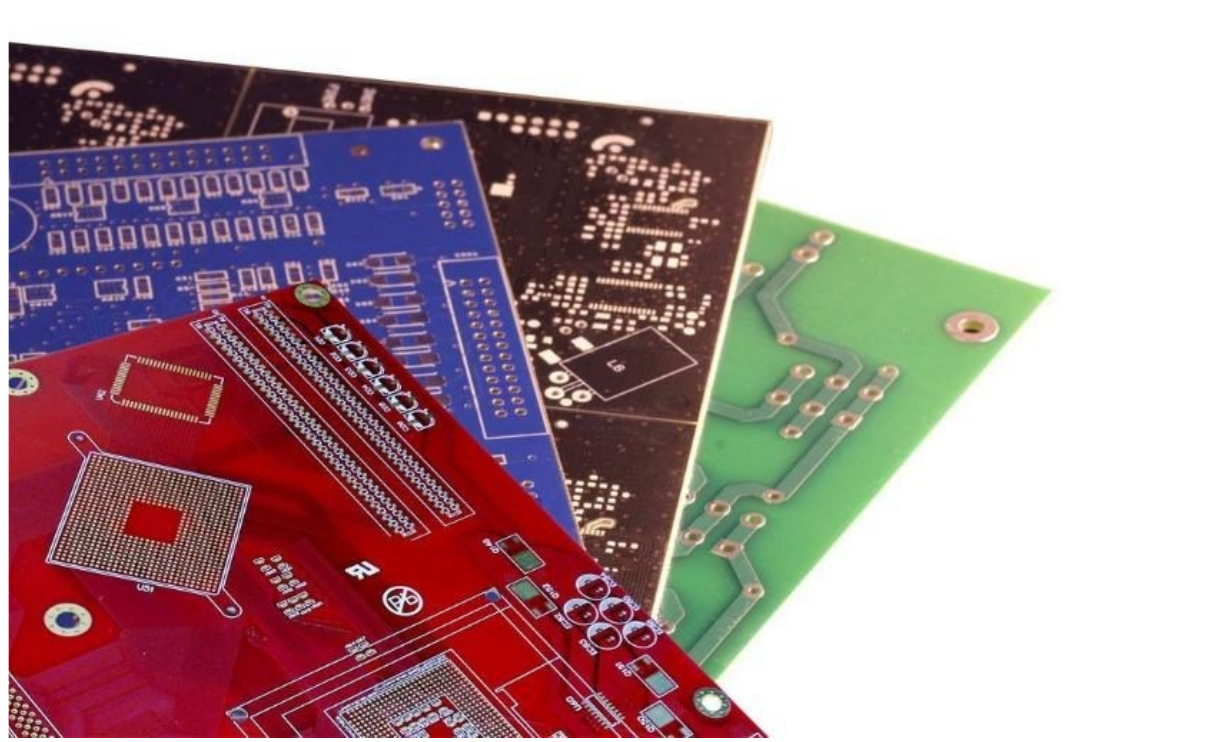
\includegraphics[max width=\linewidth,max height=0.82\textheight]{figuras/figura-01.png}
\label{fig:01}
\caption{Figura 1: Exemplos de PCBs}
\end{figure}

\hypertarget{camada-de-serigrafia}{%
\subsection{Camada de serigrafia}\label{camada-de-serigrafia}}

A camada de serigrafia é composta por tinta aplicada na superfície da PCB, destinada a fornecer informações úteis, como identificação de componentes, orientações de montagem e dados de fabricação. Essa camada desempenha um papel crucial na montagem e manutenção de dispositivos eletrônicos, facilitando a localização precisa de componentes e contribuindo para uma montagem eficiente e com menor probabilidade de erros.

Ao compreender os principais elementos das Placas de Circuito Impresso e suas funções, é possível garantir que o processo de fabricação de PCBs resulte em produtos de alta qualidade, atendendo às demandas específicas de cada projeto eletrônico.

\begin{figure}[H]
\centering
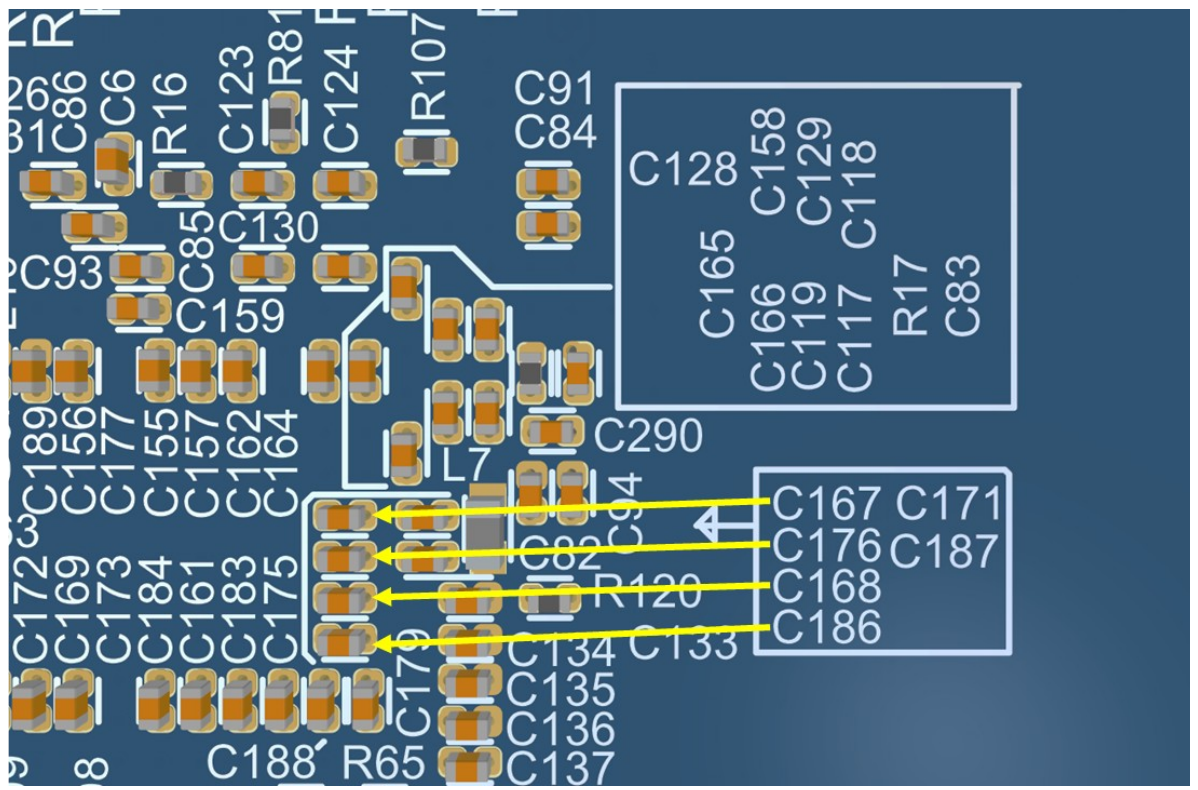
\includegraphics[max width=\linewidth,max height=0.82\textheight]{figuras/figura-02.png}
\label{fig:02}
\caption{Figura 2: Exemplos de serigrafias}
\end{figure}

\hypertarget{acabamento-de-superfuxedcie}{%
\subsection{Acabamento de superfície}\label{acabamento-de-superfuxedcie}}

Surface finish, ou Acabamento de Superfície, compõe uma interface crítica entre os componentes e o local onde serão posicionados para solda, também chamada de SMOBC (Solder Mask Over Bare Copper) -- Máscara de solda sobre cobre exposto. Essa superfície, sem nenhum tratamento, ficaria com os pads de cobre expostos, o que resultaria em oxidação, deterioração e consequente perda de funcionalidade.

O acabamento de superfície possui essencialmente duas funções:

\begin{itemize}
\tightlist
\item
  Proteger o circuito de cobre exposto;
\item
  Prover uma superfície com maior solderabilidade, bem como reforçar o processo de montagem, promovendo uma junta de solda confiável com alto desempenho da PCB a longo prazo. O processo de acabamento superficial consiste em cobrir com metal o material
  orgânico os elementos de cobre não cobertos pela máscara de solda. Este processo protege o cobre e facilita a soldagem dos componentes seja pelo processo manual, forno ou outra técnica.
\end{itemize}

As técnicas mais comuns para realizar o acabamento superficial são:

\begin{itemize}
\tightlist
\item
  \textbf{HASL/HASL Lead free (Hot Air Solder Level)}
\end{itemize}

\begin{figure}[H]
\centering
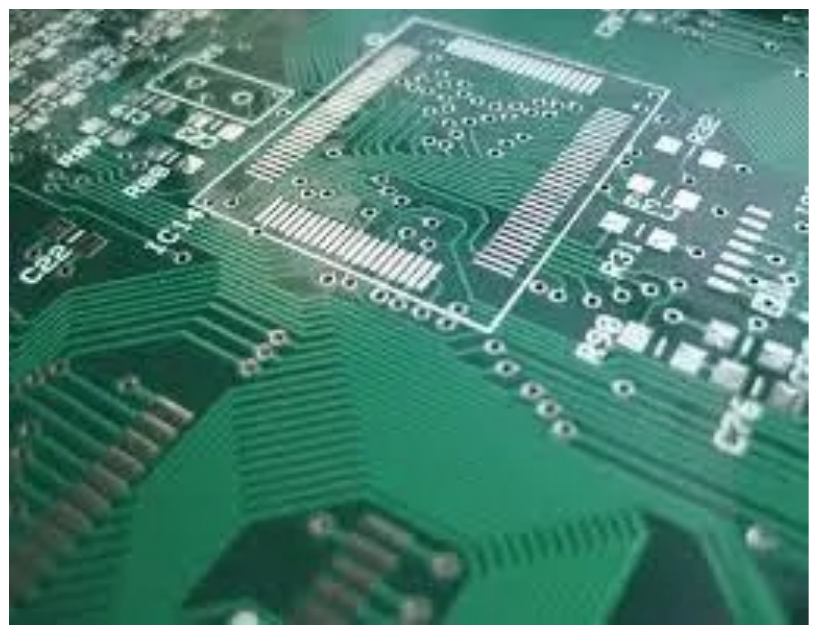
\includegraphics[max width=\linewidth,max height=0.82\textheight]{figuras/figura-03.png}
\label{fig:03}
\caption{Figura 3: Hot Air Solder Level-A}
\end{figure}

\begin{figure}[H]
\centering
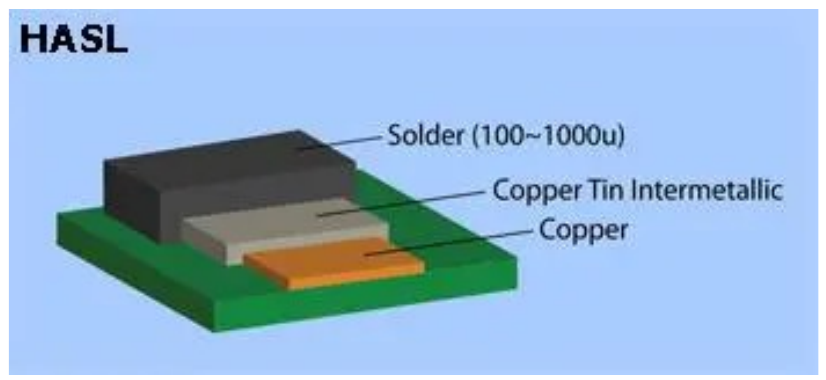
\includegraphics[max width=\linewidth,max height=0.82\textheight]{figuras/figura-04.png}
\label{fig:04}
\caption{Figura 4: Hot Air Solder Level-B}
\end{figure}

\begin{itemize}
\tightlist
\item
  \textbf{Imersão em Estanho}
\end{itemize}

\begin{figure}[H]
\centering
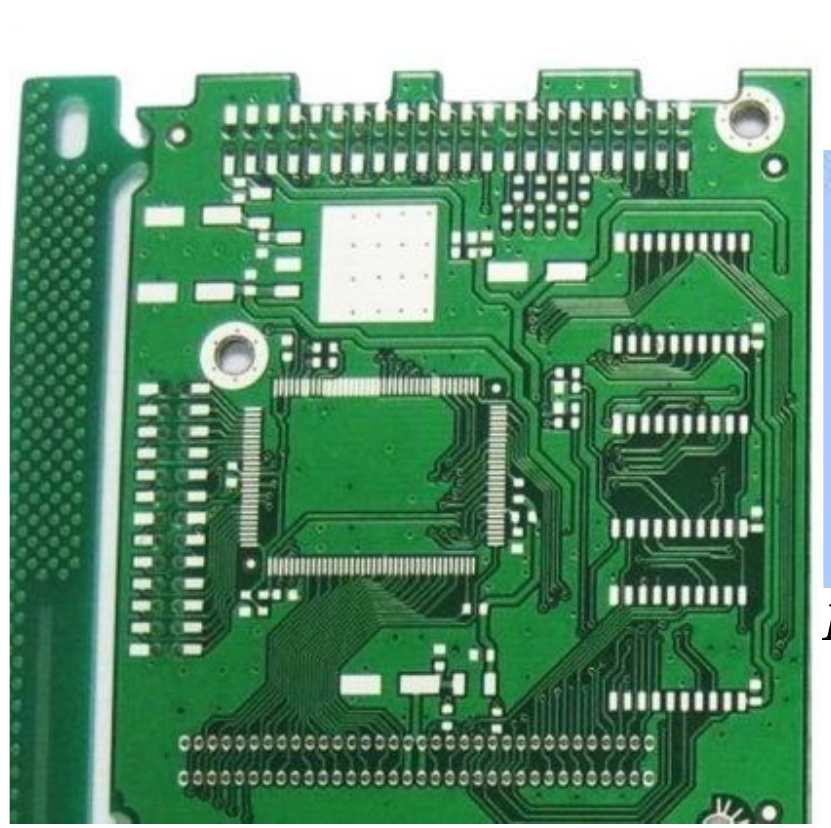
\includegraphics[max width=\linewidth,max height=0.82\textheight]{figuras/figura-05.png}
\label{fig:05}
\caption{Figura 5: Imersão em Estanho-A}
\end{figure}

\begin{figure}[H]
\centering
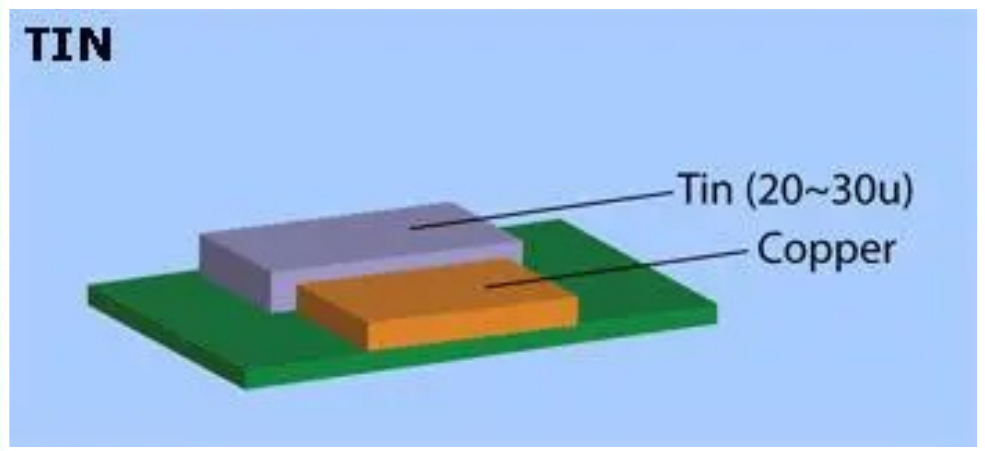
\includegraphics[max width=\linewidth,max height=0.82\textheight]{figuras/figura-06.png}
\label{fig:06}
\caption{Figura 6: Imersão em Estanho-B}
\end{figure}

\begin{itemize}
\tightlist
\item
  \textbf{Imersão em Prata}
\end{itemize}

\begin{figure}[H]
\centering
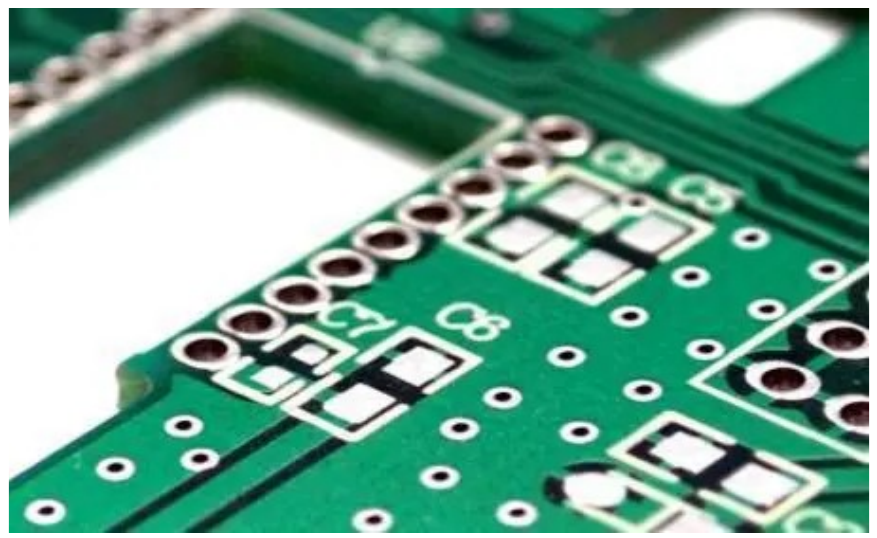
\includegraphics[max width=\linewidth,max height=0.82\textheight]{figuras/figura-07.png}
\label{fig:07}
\caption{Figura 7: Imersão em Prata-A}
\end{figure}

\begin{figure}[H]
\centering
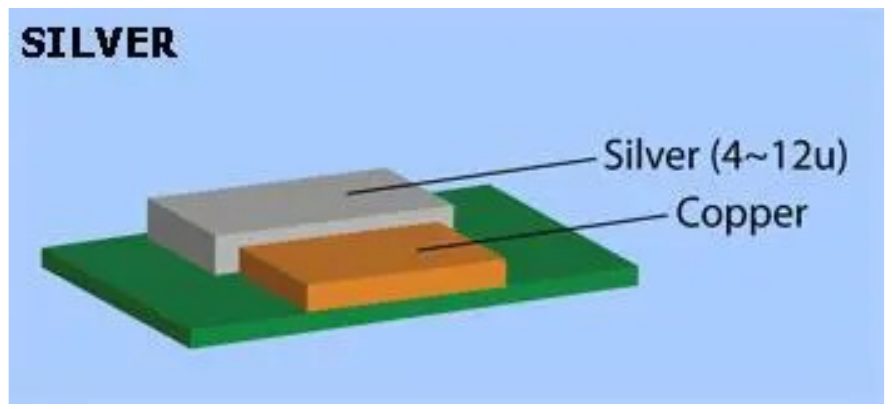
\includegraphics[max width=\linewidth,max height=0.82\textheight]{figuras/figura-08.png}
\label{fig:08}
\caption{Figura 8: Imersão em Prata-B}
\end{figure}

\begin{itemize}
\tightlist
\item
  \textbf{OSP (Organic Solderability Preservative)}
\end{itemize}

\begin{figure}[H]
\centering
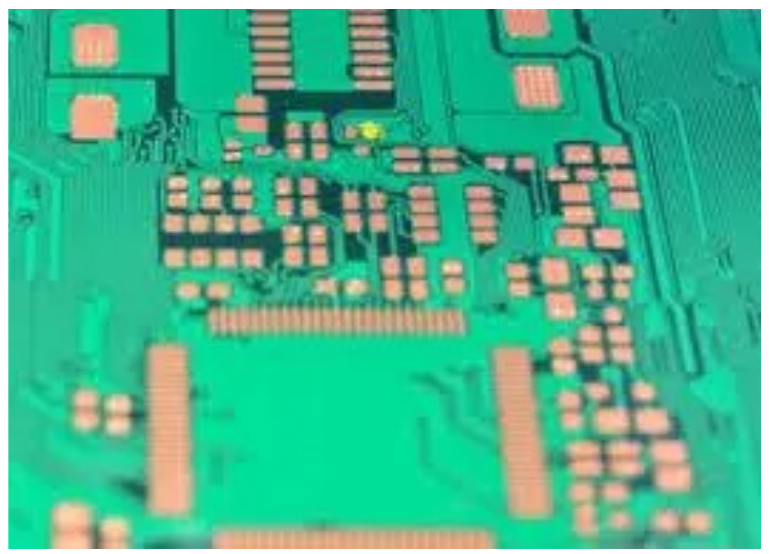
\includegraphics[max width=\linewidth,max height=0.82\textheight]{figuras/figura-09.png}
\label{fig:09}
\caption{Figura 9: Organic Solderability Preservative-A}
\end{figure}

\begin{figure}[H]
\centering
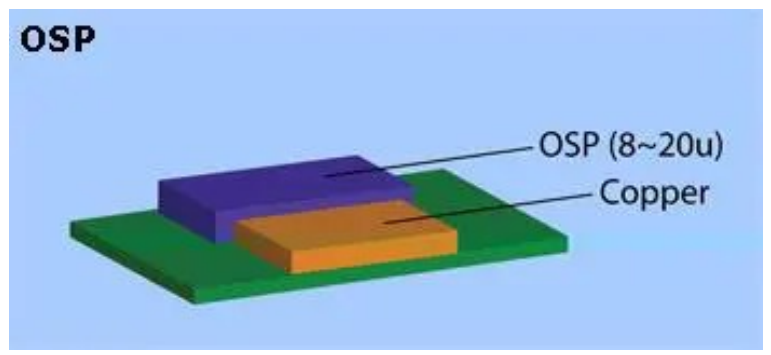
\includegraphics[max width=\linewidth,max height=0.82\textheight]{figuras/figura-10.png}
\label{fig:10}
\caption{Figura 10: Organic Solderability Preservative-B}
\end{figure}

\begin{itemize}
\tightlist
\item
  \textbf{GOLD -- ENIG (Electroless Nickel Immersion Gold)}
\end{itemize}

\begin{figure}[H]
\centering
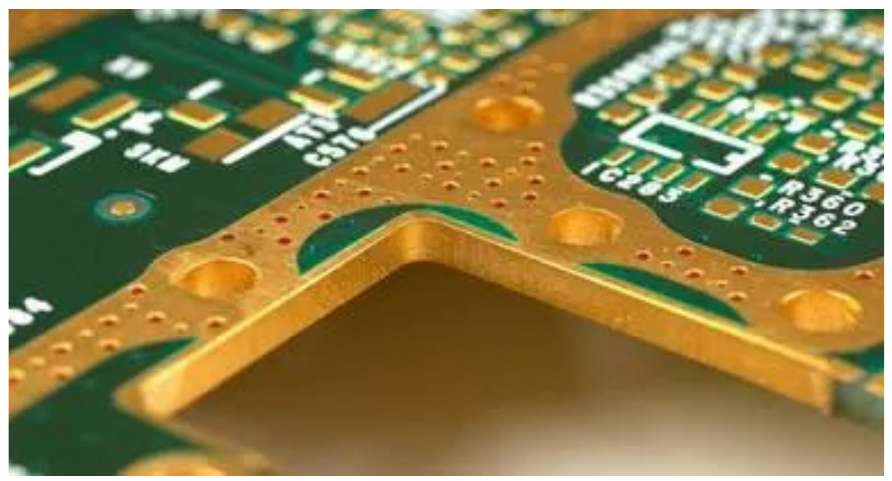
\includegraphics[max width=\linewidth,max height=0.82\textheight]{figuras/figura-11.png}
\label{fig:11}
\caption{Figura 11: Electroless Nickel Immersion Gold) - A}
\end{figure}

\begin{figure}[H]
\centering
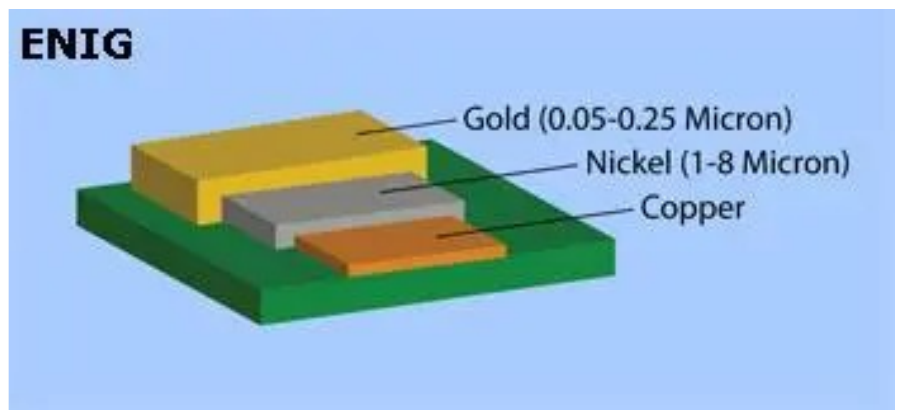
\includegraphics[max width=\linewidth,max height=0.82\textheight]{figuras/figura-12.png}
\label{fig:12}
\caption{Figura 12: Electroless Nickel Immersion Gold) - B}
\end{figure}

•\emph{Immersion Gold) - B}

\emph{Immersion Gold) - A}

\hypertarget{enepig-electroless-nickel-electroless}{%
\subsubsection{ENEPIG (Electroless Nickel Electroless}\label{enepig-electroless-nickel-electroless}}

\hypertarget{palladium-immersion-gold}{%
\subsubsection{Palladium Immersion Gold)}\label{palladium-immersion-gold}}

\begin{figure}[H]
\centering
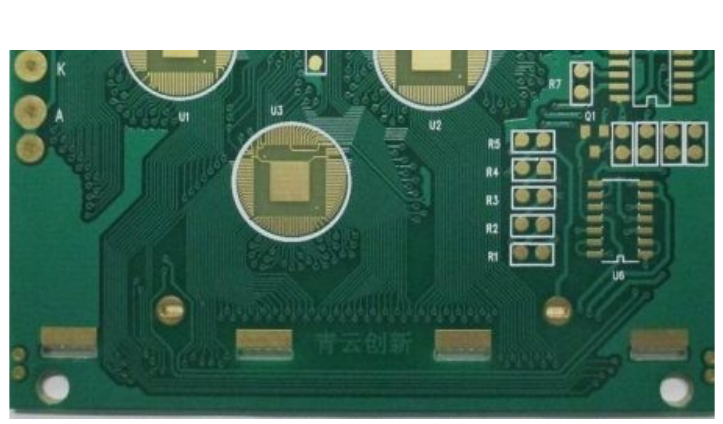
\includegraphics[max width=\linewidth,max height=0.82\textheight]{figuras/figura-13.png}
\label{fig:13}
\caption{Figura 13: Electroless Nickel Electroless Palladium Immersion Gold-A}
\end{figure}

\begin{figure}[H]
\centering
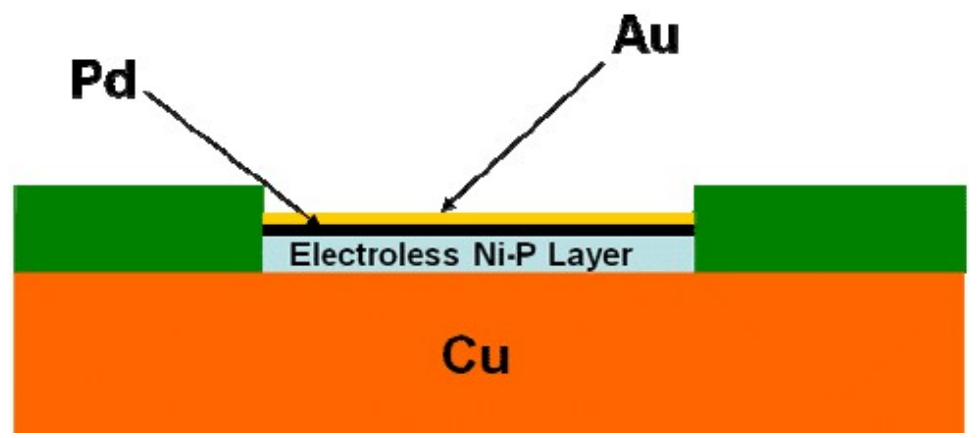
\includegraphics[max width=\linewidth,max height=0.82\textheight]{figuras/figura-14.png}
\label{fig:14}
\caption{Figura 14: Electroless Nickel Electroless Palladium Immersion Gold-B}
\end{figure}

\begin{itemize}
\tightlist
\item
  \textbf{Gold -- Hard Gold}
\end{itemize}

\begin{figure}[H]
\centering
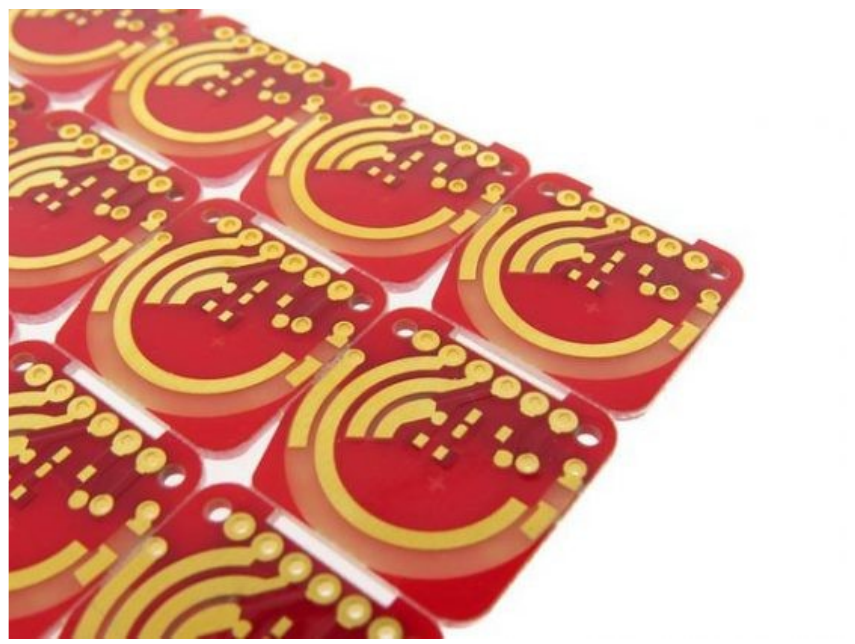
\includegraphics[max width=\linewidth,max height=0.82\textheight]{figuras/figura-15.png}
\label{fig:15}
\caption{Figura 15: Hard Gold-A}
\end{figure}

\begin{figure}[H]
\centering
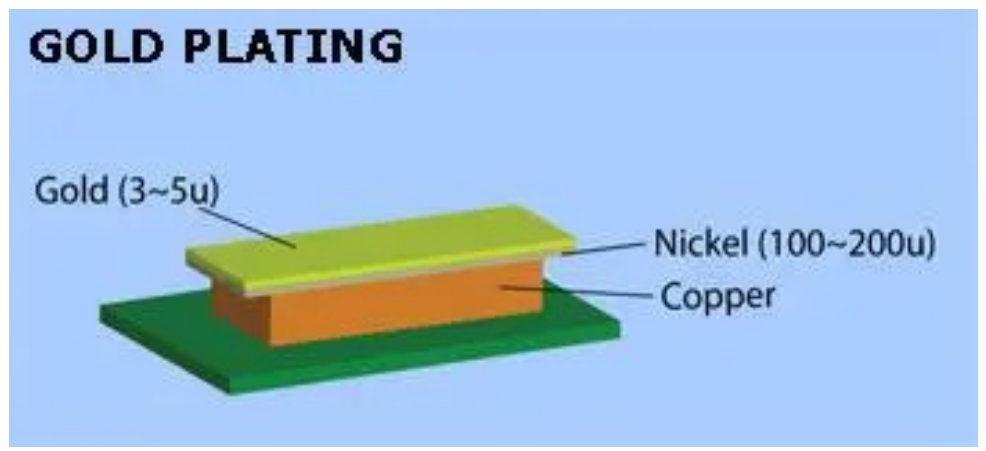
\includegraphics[max width=\linewidth,max height=0.82\textheight]{figuras/figura-16.png}
\label{fig:16}
\caption{Figura 16: Hard Gold-B}
\end{figure}

\hypertarget{normas-ipc}{%
\section{Normas IPC}\label{normas-ipc}}

Uma placa que funciona na bancada não é automaticamente uma placa que pode ser fabricada em série. Para que projetista, fabricante e montador cheguem ao mesmo entendimento sobre o que é uma placa \textbf{aceitável}, a indústria eletrônica se apoia em normas --- e a mais difundida delas é publicada pela \textbf{IPC}.

\hypertarget{o-que-uxe9-a-ipc}{%
\subsection{O que é a IPC}\label{o-que-uxe9-a-ipc}}

A IPC é a associação global da indústria de interconexão eletrônica. O nome veio de \emph{Institute for Printed Circuits} e depois foi alterado para \emph{Institute for Interconnecting and Packaging Electronic Circuits}; hoje a sigla é usada como nome próprio da organização.

Trata-se de uma associação mantida por seus membros, que publica especificações de forma periódica. As normas IPC são as regras \textbf{mais amplamente aceitas} pela indústria eletrônica e cobrem todas as etapas do ciclo de desenvolvimento de um produto: projeto, compras, montagem, empacotamento e inspeção. Segui-las ajuda a fabricar placas seguras, confiáveis e de alta qualidade --- e, para o projetista, produz um efeito prático imediato: \textbf{mantém projetista e fabricante no mesmo entendimento} sobre o que a placa precisa cumprir.

\begin{quadro}{blue!55!black}{Por que isso importa no seu projeto}
Uma norma não é uma formalidade. As classes IPC existem porque a
\textbf{mesma} placa pode ser considerada aprovada ou reprovada
dependendo do critério adotado. Ao especificar a classe, você deixa
explícito qual nível de inspeção e qual tolerância a defeito são
aceitáveis para o seu produto --- e evita que cada lado julgue a placa
por uma régua diferente.
\end{quadro}

\hypertarget{as-classes-de-qualidade}{%
\subsection{As classes de qualidade}\label{as-classes-de-qualidade}}

A \textbf{IPC-6011} descreve as classes de PCB e os \textbf{defeitos permitidos} em cada tipo de placa. São três classes, com o acréscimo posterior de uma quarta, definida pela \textbf{IPC-6012}:

\begingroup\scriptsize\begin{longtable}[]{@{}
  >{\raggedright\arraybackslash}p{(\columnwidth - 4\tabcolsep) * \real{0.1099}}
  >{\raggedright\arraybackslash}p{(\columnwidth - 4\tabcolsep) * \real{0.2637}}
  >{\raggedright\arraybackslash}p{(\columnwidth - 4\tabcolsep) * \real{0.6264}}@{}}
\toprule\noalign{}
\begin{minipage}[b]{\linewidth}\raggedright
Classe
\end{minipage} & \begin{minipage}[b]{\linewidth}\raggedright
Aplicação típica
\end{minipage} & \begin{minipage}[b]{\linewidth}\raggedright
Confiabilidade exigida e defeitos admitidos
\end{minipage} \\
\midrule\noalign{}
\endhead
\bottomrule\noalign{}
\endlastfoot
\textbf{Classe 1} & Produtos eletrônicos de uso geral --- controles remotos de TV, lâmpadas LED, brinquedos infantis & Vida útil limitada e função simples. Admite vários defeitos cosméticos, desde que não afetem o funcionamento; a confiabilidade não é fator crítico. É a placa mais barata de fabricar. \\
\textbf{Classe 2} & Produtos eletrônicos de serviço dedicado --- notebooks, smartphones, tablets, equipamentos de comunicação & Confiabilidade maior e vida útil estendida; normas mais rigorosas que a classe 1, mas ainda se admitem algumas imperfeições cosméticas. O serviço ininterrupto é preferível, porém não crítico, e não há exposição a condições ambientais extremas. \\
\textbf{Classe 3} & Produtos eletrônicos de alto desempenho --- suporte à vida, equipamentos militares, monitoramento eletrônico, automotivo & Deve fornecer desempenho contínuo, ou sob demanda, \textbf{sem parada} do equipamento; o ambiente de uso pode ser excepcionalmente severo. Exige níveis elevados de inspeção e ensaio, o que a torna altamente confiável. \\
\textbf{Classe 3/A} & Circuitos impressos de uso espacial e aviônica militar (IPC-6012) --- aeroespacial, sistemas aéreos militares, sistemas de mísseis & Categoria mais alta para circuitos impressos. Critérios de fabricação muito rigorosos, pois a placa deve continuar operando em condições críticas. Consideravelmente mais cara, por precisar estar próxima da perfeição. \\
\end{longtable}\endgroup

A diferença central entre as classes \textbf{não está no desenho da placa, e sim no grau de inspeção}: são as classes que definem quais defeitos são admissíveis durante a fabricação.

Vale desfazer um equívoco comum: as classes 3 e 3/A são usadas principalmente em equipamentos militares e aeroespaciais, mas \textbf{não são exclusivas} dessas áreas. Elas podem ser aplicadas a qualquer produto --- inclusive aos exemplos citados na classe 2 ---, porém deixam de ser economicamente viáveis pelo esforço de fabricação e de inspeção que exigem.

\hypertarget{como-escolher-a-classe}{%
\subsection{Como escolher a classe}\label{como-escolher-a-classe}}

Ao escolher a classe, o projetista está escolhendo a \textbf{vida útil} do produto. Muitas vezes a classe 2 atende a todos os requisitos e sai mais econômica. Se, além de a aplicação ser crítica, espera-se que a placa dure muitos anos, a classe 3 passa a ser a escolha adequada. O ambiente em que o produto vai operar também precisa entrar na conta, porque é ele que determina o grau de confiabilidade exigido do projeto.

\begin{quadro}{green!50!black}{Qual classe escolher}
A escolha é econômica antes de ser técnica. A \textbf{classe 2} costuma
atender à maior parte dos produtos --- e sai mais barata. Reserve a
\textbf{classe 3} para aplicações críticas ou para produtos que precisem
durar muitos anos: o material de referência cita a fronteira de
\textbf{15 anos} como um dos critérios de decisão. O ambiente de
operação do produto é o outro critério a considerar.
\end{quadro}

\hypertarget{onde-a-ipc-aparece-na-pruxe1tica}{%
\subsection{Onde a IPC aparece na prática}\label{onde-a-ipc-aparece-na-pruxe1tica}}

Duas situações concretas em que a norma entra no dia a dia do projetista:

\begin{itemize}
\tightlist
\item
  \textbf{Anel anular:} a IPC define a posição dos furos sobre a ilha de solda (\emph{pad}) e
  a largura do anel externo que resta depois da furação. Quando a ilha não circunda completamente o furo, tem-se um \emph{annular ring breakout} --- condição que a norma trata explicitamente, com limites de aceitação próprios para cada classe.
\item
  \textbf{Juntas de solda e defeitos aceitáveis:} a IPC trata separadamente os defeitos
  que comprometem o desempenho da placa e as imperfeições puramente cosméticas, e estabelece padrões de aceitação para os processos de montagem. O \textbf{mesmo} defeito pode ser aprovado na classe 1 e reprovado na classe 3: o defeito não muda, o critério é que muda.
\end{itemize}

O Capítulo 7 traz os valores de anel anular e de furação praticados por um fabricante real --- é com esses números, e não com valores arbitrários, que o seu projeto é conferido no DRC.

Fonte: IPC, \emph{IPC Class 3 Design Guide} (material de apoio da disciplina).

\hypertarget{categorias-de-pcbs}{%
\section{Categorias de PCBs}\label{categorias-de-pcbs}}

\begin{itemize}
\tightlist
\item
  \textbf{PCBs de Face Única}: Contêm uma única camada de cobre em um dos lados do substrato, utilizadas em circuitos simples e de baixo custo.
\item
  \textbf{PCBs de Dupla Face}: Possuem trilhas condutoras em ambos os lados do substrato, conectadas por vias, sendo amplamente usadas em designs intermediários.
\item
  \textbf{PCBs Multicamadas}: Incorporam múltiplas camadas de cobre intercaladas com materiais isolantes, permitindo designs mais complexos e de alta densidade, comuns em dispositivos como smartphones e computadores. Compreender os princípios e os elementos que compõem as PCBs é o primeiro
  passo para dominar o design dessas placas essenciais.
\end{itemize}

\hypertarget{boas-pruxe1ticas-de-design}{%
\chapter{Boas Práticas de Design}\label{boas-pruxe1ticas-de-design}}

O sucesso de um projeto de PCB depende não apenas de sua funcionalidade, mas também da facilidade de produção e da confiabilidade durante o uso. Para garantir que sua placa seja eficiente, econômica e durável, é essencial adotar boas práticas de design. Neste capítulo, abordaremos estratégias para evitar falhas comuns e melhorar a manufaturabilidade do seu projeto.

\hypertarget{planejamento-inicial}{%
\section{Planejamento Inicial}\label{planejamento-inicial}}

Antes de começar o roteamento, faça um planejamento cuidadoso do layout da placa, colocando os componentes de forma lógica e otimizada. Agrupe componentes relacionados e posicione-os de maneira que minimize os trajetos de conexão.

\begin{itemize}
\item
  Defina as camadas de PCB: determine quantas camadas de PCB você irá utilizar. Camadas adicionais podem permitir trajetos mais curtos e reduzir a interferência entre sinais.
\item
  Rotas Críticas: identifique os sinais críticos, como sinais de alta velocidade, alimentação e terra. Roteie esses sinais primeiro, minimizando interferências e distâncias.
\item
  Plano de Terra Adequado: certifique-se de criar uma área de plano de terra sólido na placa, conectando-a adequadamente a todos os pontos de terra. Isso ajuda a reduzir interferências e proporciona um retorno confiável para os sinais.
\item
  Rotas Diretas e Curtas: mantenha os trajetos de roteamento o mais curtos e diretos possível para evitar atrasos de sinal, interferência eletromagnética e perda de sinal.
\item
  Separação de Sinais: mantenha diferentes tipos de sinais separados para reduzir a interferência. Isso é especialmente importante para sinais analógicos e digitais, que podem interferir entre si.
\item
  Regras de Projeto: defina regras de projeto no software de layout de PCB para garantir espaçamentos adequados entre trilhas, vias e componentes, evitando problemas como curtos-circuitos.
\item
  Uso de Vias: utilize vias para conectar camadas diferentes de PCB. Coloque as vias de forma eficiente, evitando congestionamentos, e distribua-as uniformemente para ajudar na distribuição de energia e terra.
\item
  Roteamento Manual vs.~Automático: embora o roteamento automático possa ser útil, em muitos casos, um roteamento manual oferece mais controle sobre o layout. Comece com o roteamento manual e use o roteamento automático como uma ferramenta auxiliar, se necessário.
\item
  Revisão e Simulação: antes de finalizar o layout, revise cuidadosamente todas as trilhas, vias e conexões. Além disso, é recomendável realizar simulações para verificar o desempenho do circuito, especialmente em termos de integridade de sinal.
\end{itemize}

\hypertarget{planejamento-do-design}{%
\section{Planejamento do Design}\label{planejamento-do-design}}

Antes de começar a desenhar a PCB, tenha um esquema elétrico bem elaborado e documentado. Planeje o layout considerando:

\begin{itemize}
\item
  \textbf{Fluxo do sinal:} Posicione os componentes para otimizar o percurso das conexões.
\item
  \textbf{Gerenciamento de espaço:} Evite agrupamentos excessivos e deixe espaço suficiente para trilhas e pads.
\item
  \textbf{Restrições mecânicas:} Considere dimensões da placa, pontos de fixação e encaixes.
\end{itemize}

\hypertarget{separauxe7uxe3o-de-uxe1reas-funcionais}{%
\section{Separação de Áreas Funcionais}\label{separauxe7uxe3o-de-uxe1reas-funcionais}}

Divida a placa em zonas, agrupando componentes relacionados. Por exemplo:

\begin{itemize}
\tightlist
\item
  Zona de potência: Para fontes e reguladores.
\item
  Zona de sinal: Para circuitos de baixa tensão e alta frequência.
\item
  Zona de controle: Para microcontroladores e circuitos lógicos. Essa separação reduz interferências e facilita o diagnóstico e a manutenção.
  Veja a figura.
\end{itemize}

\begin{figure}[H]
\centering
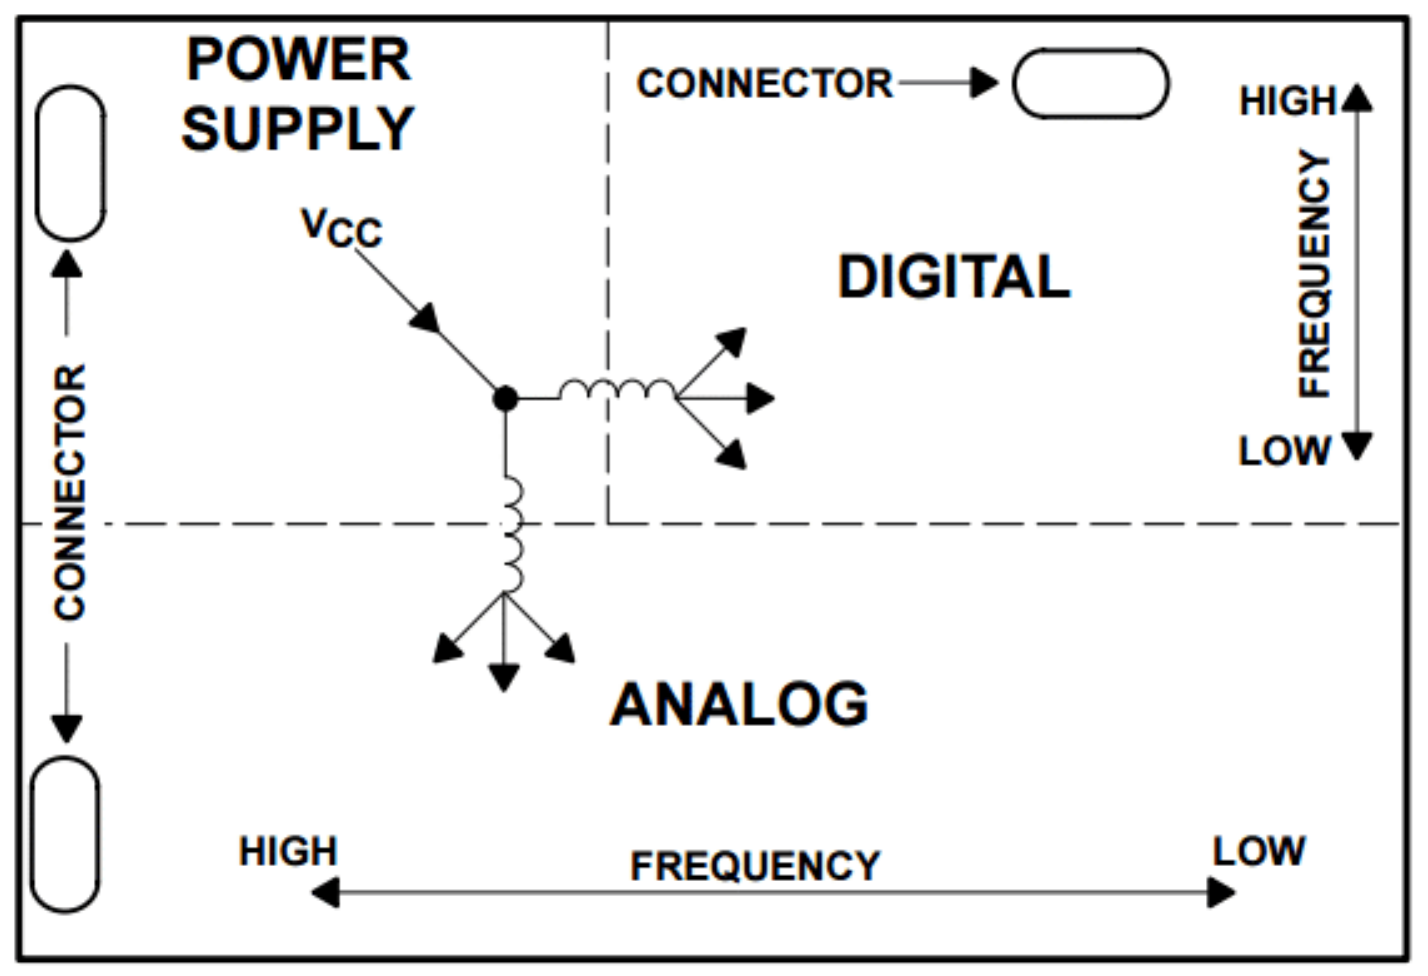
\includegraphics[max width=\linewidth,max height=0.82\textheight]{figuras/figura-17.png}
\label{fig:17}
\caption{Figura 17: Separação dos componentes em grupos de função}
\end{figure}

\hypertarget{largura-de-trilhas-e-distuxe2ncia-muxednima}{%
\section{Largura de Trilhas e Distância Mínima}\label{largura-de-trilhas-e-distuxe2ncia-muxednima}}

Calcule a largura das trilhas com base na corrente que elas suportarão, mas a largura necessária \textbf{não depende só da corrente}: dependem também a elevação de temperatura admitida, a espessura do cobre e a camada (externa ou interna). Trilhas mais largas são necessárias para correntes maiores. Use a tabela ou calculadora do fabricante para o valor final. Além disso:

\begin{itemize}
\item
  Respeite as distâncias mínimas entre trilhas para evitar curtos-circuitos.
\item
  Utilize ferramentas de verificação de regras de design (DRC) no software para garantir conformidade com os requisitos do fabricante ou equipamento a ser utilizado na fabricação.
\end{itemize}

\hypertarget{gerenciamento-tuxe9rmico}{%
\section{Gerenciamento Térmico}\label{gerenciamento-tuxe9rmico}}

\begin{itemize}
\tightlist
\item
  Posicione dissipadores de calor e vias térmicas próximas a componentes que geram muito calor.
\item
  Utilize planos de aterramento e alimentação para distribuir o calor de forma eficiente. Evite áreas isoladas de cobre que podem atuar como hotspots.
\end{itemize}

\hypertarget{trilhas-de-alimentauxe7uxe3o}{%
\section{Trilhas de Alimentação}\label{trilhas-de-alimentauxe7uxe3o}}

Mantenha as trilhas de alimentação largas o suficiente para minimizar a queda de tensão devido à resistência.

\hypertarget{planos-de-terra}{%
\section{Planos de Terra}\label{planos-de-terra}}

\begin{itemize}
\tightlist
\item
  \textbf{Plano de Terra Sólido:} Crie um plano de terra contínuo em uma camada interna da PCB para fornecer um retorno eficiente para os sinais.
\item
  \textbf{Conexão de Terra:} Conecte o plano de terra a todos os pontos de terra do circuito. Use várias vias para conectar as camadas de terra.
\end{itemize}

\begin{quadro}{red!65!black}{Plano de terra: um só, contínuo}
Prefira \textbf{um plano de terra contínuo} a dividi-lo em regiões
analógica e digital. O plano contínuo minimiza a impedância entre dois
pontos de terra quaisquer e garante o caminho de retorno da corrente. A
separação em regiões só se justifica em casos específicos e precisa de
\textbf{um único ponto de interligação controlado} entre elas: dividir
sem esse ponto transforma a emenda em antena e piora a integridade do
sinal.
\end{quadro}

\begin{itemize}
\tightlist
\item
  \textbf{Costura de vias (\emph{stitching}):} posicione vias de terra na origem e no destino do sinal, para que a corrente de retorno possa voltar pelo plano de referência.
\end{itemize}

\begin{figure}[H]
\centering
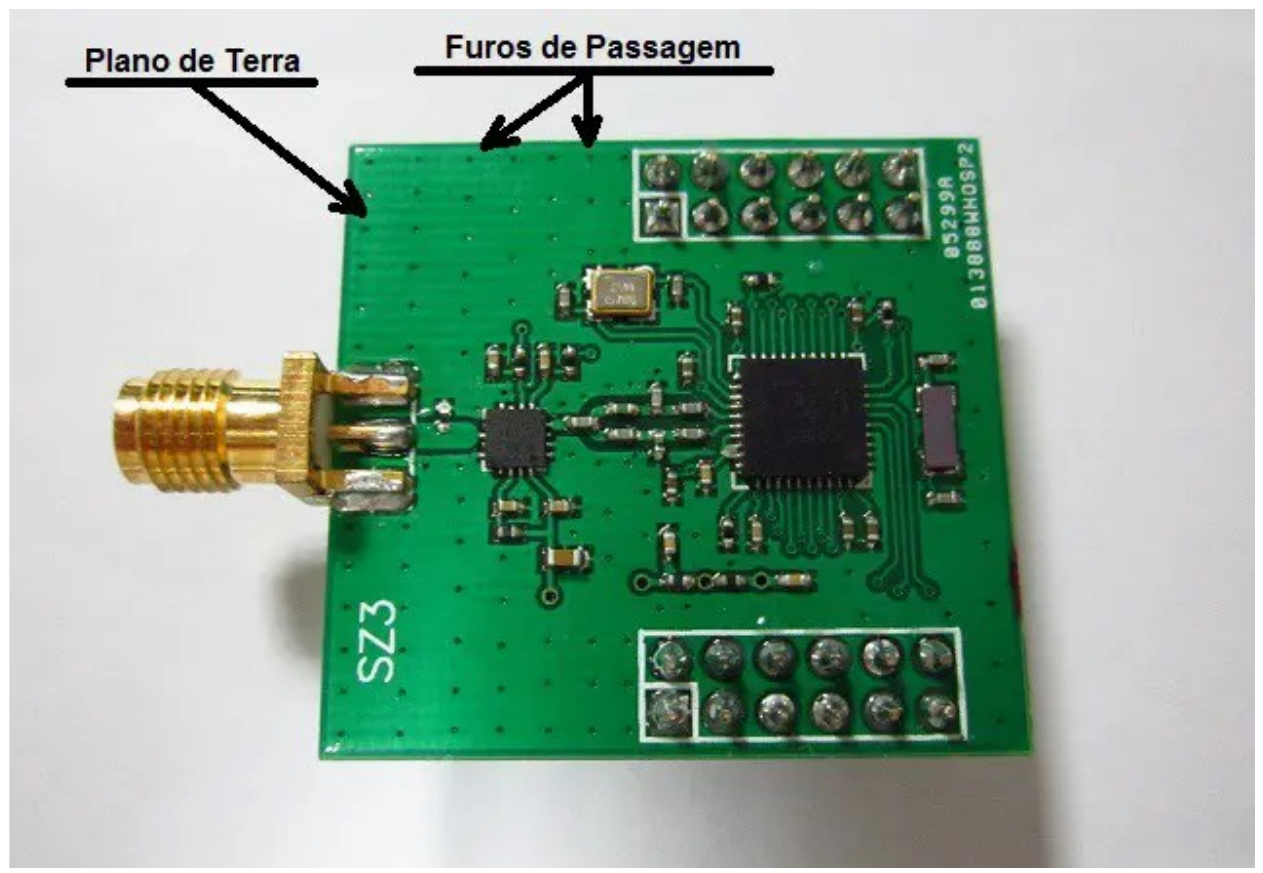
\includegraphics[max width=\linewidth,max height=0.82\textheight]{figuras/figura-18.png}
\label{fig:18}
\caption{Figura 18: Plano de terra e furos de passagem}
\end{figure}

\begin{figure}[H]
\centering
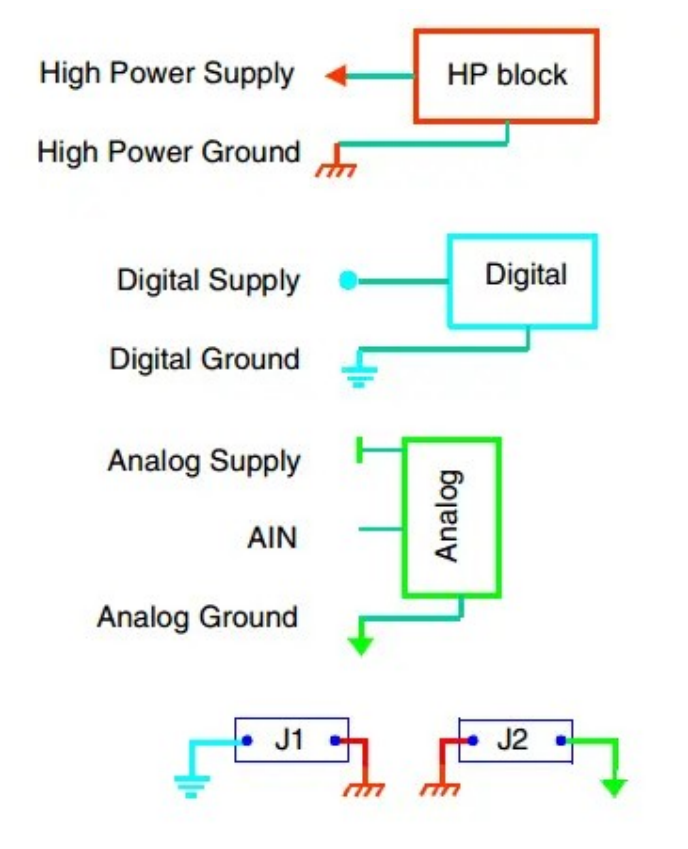
\includegraphics[max width=\linewidth,max height=0.82\textheight]{figuras/figura-19.png}
\label{fig:19}
\caption{Figura 19: Cada seção do circuito deve ter seu plano de terra, havendo a interligação entre eles}
\end{figure}

\begin{figure}[H]
\centering
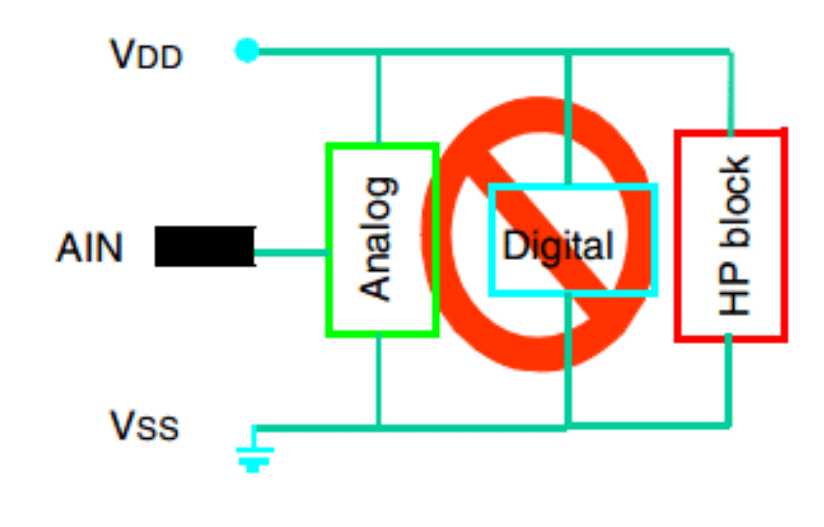
\includegraphics[max width=\linewidth,max height=0.82\textheight]{figuras/figura-20.png}
\label{fig:20}
\caption{Figura 20: A ligação de todos os grupos na mesma linha de alimentação e terra não é recomendada}
\end{figure}

\hypertarget{minimizauxe7uxe3o-de-interferuxeancias}{%
\section{Minimização de Interferências}\label{minimizauxe7uxe3o-de-interferuxeancias}}

\begin{itemize}
\tightlist
\item
  \textbf{Roteamento Paralelo e Perpendicular:} o acoplamento indutivo e capacitivo (\emph{crosstalk}) \textbf{cresce com o comprimento em que duas trilhas correm paralelas e próximas}, e é mínimo quando elas se cruzam perpendicularmente. Portanto: mantenha o trecho paralelo entre trilhas sensíveis o mais curto possível, cruze-as em ângulo reto quando o cruzamento for inevitável e afaste-as onde o paralelismo for necessário.
\end{itemize}

\begin{quadro}{green!50!black}{Regra prática: espaçamento entre trilhas (3W)}
Para reduzir \emph{crosstalk}, mantenha o centro de uma trilha a pelo
menos \textbf{3 vezes a sua largura (3W)} de outra trilha; \textbf{2W} é
o mínimo aceitável. A regra \textbf{não} se aplica ao espaçamento
interno de um par diferencial.
\end{quadro}

\begin{itemize}
\item
  Trilhas de Sinal de Referência: Para sinais diferenciais, como USB ou Ethernet, mantenha as trilhas de sinal e referência equidistantes e paralelas respeitando a impedância necessária.
\item
  \textbf{Referência de terra próxima ao sinal:} o plano de terra adjacente é o \textbf{caminho de retorno da corrente} e deve ficar contínuo e próximo da trilha de sinal --- afastar o sinal do plano de referência aumenta a impedância e a emissão. O que precisa de afastamento são as trilhas de \textbf{outros sinais}, não o plano de referência.
\item
  \textbf{Use Camadas de Sinal:} Utilize camadas de sinal adjacentes para trilhas de sinais complementares, como um plano de terra entre camadas de sinal.
\item
  \textbf{Filtros e Blindagem:} Utilize componentes de filtragem, como capacitores e indutores, para reduzir o ruído de alta frequência. Considere a utilização de placas de blindagem para componentes sensíveis.
\item
  \textbf{Roteamento Diferencial:} Para sinais de alta velocidade, como USB, HDMI ou PCIe, utilize roteamento diferencial e respeita a impedância pelo tipo de interface para reduzir a interferência e melhorar a integridade do sinal.
\item
  Mantenha trilhas de alta frequência curtas e bem separadas de sinais sensíveis.
\item
  \textbf{Use planos de referência (GND)} contínuos para reduzir ruídos e melhorar a integridade do sinal.
\item
  \textbf{Adicione capacitores de desacoplamento} próximos aos pinos de alimentação de componentes IC.
\item
  \textbf{Coloque sinais e trilhas de terra relacionados próximos} um do outro para minimizar a impedância e a interferência
\end{itemize}

\hypertarget{otimizauxe7uxe3o-de-pads-e-vias}{%
\section{Otimização de Pads e Vias}\label{otimizauxe7uxe3o-de-pads-e-vias}}

\begin{itemize}
\tightlist
\item
  Certifique-se de que os pads sejam grandes o suficiente para facilitar a soldagem.
\item
  Evite vias muito próximas aos pads, o que pode causar problemas de soldagem.
\item
  Use vias metalizadas para conexões confiáveis entre camadas.
\end{itemize}

\hypertarget{simplificauxe7uxe3o-do-layout}{%
\section{Simplificação do Layout}\label{simplificauxe7uxe3o-do-layout}}

\begin{quadro}{orange!85!black}{Ângulos na trilha: use 45°}
Evite ângulos agudos e cantos fechados; prefira ângulos de 45°. A razão
principal é de \textbf{fabricação}: ângulos agudos formam armadilha de
ácido (\emph{acid trap}) na etapa de corrosão, o que pode supercorroer a
trilha e abrir o circuito.
\end{quadro}

\begin{itemize}
\tightlist
\item
  Minimize o uso de vias desnecessárias, pois elas aumentam o custo e podem reduzir a confiabilidade.
\end{itemize}

\hypertarget{serigrafia-clara-e-informativa}{%
\section{Serigrafia Clara e Informativa}\label{serigrafia-clara-e-informativa}}

\begin{itemize}
\tightlist
\item
  Inclua rótulos claros para identificação de componentes e orientações de montagem.
\item
  Evite sobrepor a serigrafia em pads ou vias.
\end{itemize}

\hypertarget{considerauxe7uxf5es-de-fabricauxe7uxe3o}{%
\section{Considerações de Fabricação}\label{considerauxe7uxf5es-de-fabricauxe7uxe3o}}

\begin{itemize}
\tightlist
\item
  Utilize espessuras de cobre padrão (geralmente 1 oz/ft²) para facilitar a produção.
\item
  Respeite as tolerâncias do fabricante em relação a furos, espessura de trilhas e distâncias mínimas.
\item
  Geração de arquivos de produção (Gerber) compatíveis com os requisitos da fabricante.
\end{itemize}

\hypertarget{testabilidade}{%
\section{Testabilidade}\label{testabilidade}}

Inclua pontos de teste para verificar as principais funções do circuito.

Garanta acesso físico aos pontos de teste durante a fase de inspeção e depuração.

\hypertarget{ligauxe7uxe3o-das-es-do-mcu-com-os-conectores}{%
\section{Ligação das E/S do MCU com os conectores}\label{ligauxe7uxe3o-das-es-do-mcu-com-os-conectores}}

\begin{quadro}{orange!85!black}{Nunca ligue o microcontrolador direto no conector}
Nunca ligue diretamente os terminais de um microcontrolador nos
conectores ou bornes da placa. Use uma interface entre as seções do
sistema, como mostra a Figura 21.
\end{quadro}

\begin{figure}[H]
\centering
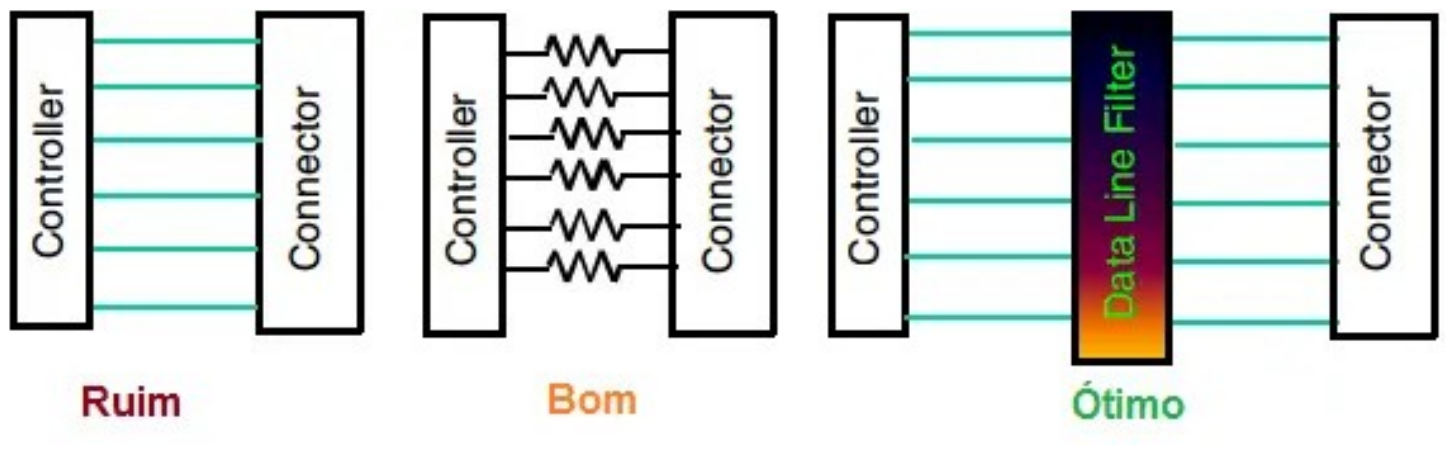
\includegraphics[max width=\linewidth,max height=0.82\textheight]{figuras/figura-21.png}
\label{fig:21}
\caption{Figura 21: É recomendado o uso de interfaces entre seções do sistema}
\end{figure}

\hypertarget{processo-buxe1sico-de-fabricauxe7uxe3o-de-pcb}{%
\chapter{Processo básico de fabricação de PCB}\label{processo-buxe1sico-de-fabricauxe7uxe3o-de-pcb}}

A fabricação de Placas de Circuito Impresso (PCB) envolve uma série de etapas cuidadosamente planejadas e executadas.

\hypertarget{etapa-fotogruxe1fica-para-criauxe7uxe3o-do-padruxe3o-de-trilhas}{%
\section{Etapa fotográfica para criação do padrão de trilhas}\label{etapa-fotogruxe1fica-para-criauxe7uxe3o-do-padruxe3o-de-trilhas}}

O processo começa com a criação de um padrão das trilhas condutoras a serem impressas na placa. Para isso, é realizada uma etapa fotográfica, onde o desenho das trilhas é transferido para uma máscara fotográfica, também conhecida como fotolito.

\hypertarget{utilizauxe7uxe3o-de-foto-resistente-e-muxe1scara-fotogruxe1fica}{%
\section{Utilização de foto-resistente e máscara fotográfica}\label{utilizauxe7uxe3o-de-foto-resistente-e-muxe1scara-fotogruxe1fica}}

A placa de cobre revestida é então preparada com uma camada de foto-resistente, um material sensível à luz que reage quando exposto à radiação ultravioleta (UV). A máscara fotográfica é posicionada sobre a placa e, em seguida, a luz UV é aplicada. As áreas do foto-resistente expostas à luz UV endurecem, enquanto as áreas protegidas pela máscara permanecem inalteradas.

\hypertarget{etapa-de-corrosuxe3o-do-cobre-com-cloreto-fuxe9rrico}{%
\section{Etapa de corrosão do cobre com cloreto férrico}\label{etapa-de-corrosuxe3o-do-cobre-com-cloreto-fuxe9rrico}}

Após a exposição à luz UV, a placa é submersa em uma solução de cloreto férrico, um agente corrosivo que remove o cobre nas áreas não protegidas pelo foto-resistente endurecido. Dessa forma, apenas as trilhas desejadas permanecem na placa.

\hypertarget{alternativas-fresagem-cnc-e-serigrafia-com-tintas-resistentes-uxe0-corrosuxe3o}{%
\section{Alternativas: Fresagem CNC e serigrafia com tintas resistentes à corrosão}\label{alternativas-fresagem-cnc-e-serigrafia-com-tintas-resistentes-uxe0-corrosuxe3o}}

Além do processo fotográfico, existem outras técnicas para a criação do padrão de trilhas nas PCBs. A fresagem CNC (Controle Numérico Computadorizado) é uma opção que utiliza máquinas de precisão para cortar diretamente o cobre, formando as trilhas. A serigrafia com tintas resistentes à corrosão é outra alternativa, onde a tinta é aplicada diretamente sobre a placa de cobre, agindo como uma máscara protetora contra a corrosão.

Ao compreender o processo básico de fabricação de PCB, é possível ter uma visão clara das etapas envolvidas na produção de placas de circuito impresso de alta qualidade, fundamentais para a indústria eletrônica atual.

\hypertarget{furos-e-vias-na-pcb}{%
\section{Furos e vias na PCB}\label{furos-e-vias-na-pcb}}

Os furos e vias desempenham um papel essencial nas placas de circuito impresso (PCBs), garantindo a conexão entre camadas e a montagem de componentes.

\hypertarget{conexuxe3o-entre-camadas-e-montagem-de-componentes}{%
\subsection{Conexão entre camadas e montagem de componentes}\label{conexuxe3o-entre-camadas-e-montagem-de-componentes}}

Os furos e vias na PCB servem para conectar as trilhas condutoras entre as diferentes camadas de uma PCB multicamadas e para fixar componentes eletrônicos na placa. Os componentes são geralmente soldados nos furos, enquanto as vias garantem a comunicação entre as camadas.

\hypertarget{perfurauxe7uxe3o-controlada-numericamente-cnc-a-partir-de-dados-do-software-cad}{%
\subsection{Perfuração controlada numericamente (CNC) a partir de dados do software CAD}\label{perfurauxe7uxe3o-controlada-numericamente-cnc-a-partir-de-dados-do-software-cad}}

A perfuração dos furos e vias nas PCBs é realizada por máquinas de perfuração controlada numericamente (CNC). Os dados para a perfuração são gerados a partir de arquivos de projeto de software CAD e convertidos em instruções específicas para a máquina CNC. Isso garante a precisão e a repetibilidade na criação dos furos e vias.

\hypertarget{vias-cegas-ou-microvias-conexuxf5es-internas-entre-camadas}{%
\subsection{Vias cegas ou microvias: conexões internas entre camadas}\label{vias-cegas-ou-microvias-conexuxf5es-internas-entre-camadas}}

Além das vias tradicionais, que atravessam todas as camadas de uma PCB, existem as vias cegas. As vias cegas são usadas para conectar trilhas condutoras entre camadas internas sem atravessar a placa inteira. Isso permite um design de PCB mais compacto e eficiente em termos de espaço.

\hypertarget{reduuxe7uxe3o-do-nuxfamero-de-tamanhos-de-furos-para-diminuir-custos}{%
\subsection{Redução do número de tamanhos de furos para diminuir custos}\label{reduuxe7uxe3o-do-nuxfamero-de-tamanhos-de-furos-para-diminuir-custos}}

Um dos fatores que afetam o custo de fabricação de uma PCB é o número de tamanhos de furos diferentes usados no projeto. Reduzir o número de tamanhos de furos pode ajudar a diminuir os custos de fabricação, pois menos ferramentas e trocas de brocas são necessárias durante o processo de perfuração. É importante equilibrar essa redução de custos com as necessidades de design e desempenho do circuito eletrônico.

Em resumo, os furos e vias são componentes cruciais na fabricação de placas de circuito impresso, garantindo a conexão entre camadas e a montagem adequada dos componentes eletrônicos. O uso de tecnologias como a perfuração controlada numericamente (CNC) e a implementação de vias cegas, além da redução do número de tamanhos de furos, pode melhorar a eficiência e reduzir os custos na fabricação de PCBs.

\hypertarget{revestimento-de-solda-e-resistuxeancia-uxe0-solda}{%
\section{Revestimento de solda e resistência à solda}\label{revestimento-de-solda-e-resistuxeancia-uxe0-solda}}

O revestimento de solda e a resistência à solda são etapas fundamentais no processo de fabricação de placas de circuito impresso (PCBs). Eles garantem a proteção das áreas não-soldadas e facilitam a soldagem de componentes.

\hypertarget{proteuxe7uxe3o-de-uxe1reas-nuxe3o-soldadas-por-meio-de-resistuxeancia-uxe0-solda}{%
\subsection{Proteção de áreas não-soldadas por meio de resistência à solda}\label{proteuxe7uxe3o-de-uxe1reas-nuxe3o-soldadas-por-meio-de-resistuxeancia-uxe0-solda}}

A resistência à solda é uma camada de material aplicada sobre a superfície da PCB para proteger as áreas não-soldadas. Essa camada ajuda a evitar a aderência de solda nas áreas indesejadas e garante que a solda seja aplicada apenas nas áreas onde os componentes devem ser fixados (máscara de solda).

Cores comuns de resistência à solda: verde escuro e vermelho -- A resistência à solda pode ser encontrada em diversas cores, sendo as mais comuns o verde escuro e o vermelho. A escolha da cor pode ser baseada em considerações estéticas, requisitos de identificação ou especificações do cliente. No entanto, a cor da resistência à solda não afeta o desempenho da PCB.

\hypertarget{estanho-ou-ouro-para-facilitar-a-soldagem-de-componentes}{%
\subsection{Estanho ou ouro para facilitar a soldagem de componentes}\label{estanho-ou-ouro-para-facilitar-a-soldagem-de-componentes}}

A fim de melhorar a adesão da solda e a qualidade das conexões elétricas, as áreas onde os componentes serão soldados recebem um revestimento de solda. Os materiais comuns utilizados para o revestimento de solda incluem o estanho e o ouro. Esses metais proporcionam uma superfície propícia para a soldagem e garantem conexões elétricas confiáveis (acabamento superficial).

Em resumo, o revestimento de solda e a resistência à solda são elementos críticos na fabricação de placas de circuito impresso, garantindo a proteção das áreas não-soldadas e facilitando a soldagem de componentes eletrônicos. A escolha dos materiais e das cores utilizadas pode variar, mas a função principal dessas camadas é garantir a qualidade e a durabilidade das conexões elétricas na PCB.

\hypertarget{serigrafia-na-pcb}{%
\section{Serigrafia na PCB}\label{serigrafia-na-pcb}}

A serigrafia é uma etapa importante no processo de fabricação de placas de circuito impresso (PCB), pois auxilia na identificação e localização de componentes durante a montagem e manutenção.

\hypertarget{impressuxe3o-de-textos-e-identificadores-na-placa}{%
\subsection{Impressão de textos e identificadores na placa}\label{impressuxe3o-de-textos-e-identificadores-na-placa}}

A serigrafia consiste em imprimir informações na superfície da PCB por meio de um processo de impressão semelhante à tela de seda. Essas informações podem incluir textos e identificadores, como a designação dos componentes, referências de pinos, logotipos da empresa e informações de conformidade.

\hypertarget{auxuxedlio-na-identificauxe7uxe3o-e-localizauxe7uxe3o-de-componentes}{%
\subsection{Auxílio na identificação e localização de componentes}\label{auxuxedlio-na-identificauxe7uxe3o-e-localizauxe7uxe3o-de-componentes}}

A serigrafia facilita a identificação e a localização dos componentes na PCB durante a montagem, teste e manutenção do dispositivo eletrônico. Ao fornecer informações claras e legíveis, os técnicos e engenheiros podem trabalhar de maneira mais eficiente, reduzindo o risco de erros na montagem e soldagem de componentes.

\hypertarget{uso-de-tela-de-seda-gerada-pelo-software-de-design-de-pcb}{%
\subsection{Uso de tela de seda gerada pelo software de design de PCB}\label{uso-de-tela-de-seda-gerada-pelo-software-de-design-de-pcb}}

Durante o processo de design da PCB, os engenheiros utilizam softwares de design de PCB para criar a tela de seda que será usada na etapa de serigrafia. Essa tela contém todas as informações necessárias para a identificação dos componentes e conexões elétricas. O arquivo gerado é então enviado ao fabricante da PCB, que utiliza a tela de seda como base para imprimir as informações na placa.

Em resumo, a serigrafia é uma etapa essencial na fabricação de placas de circuito impresso, pois facilita a identificação e localização de componentes durante a montagem e manutenção dos dispositivos eletrônicos. Através da utilização de softwares de design de PCB, os engenheiros podem criar telas de seda precisas e detalhadas que garantem a qualidade e a funcionalidade das PCBs.

\hypertarget{protuxf3tipo-de-pcb}{%
\chapter{Protótipo de PCB}\label{protuxf3tipo-de-pcb}}

A criação de protótipos de PCB é um passo fundamental no desenvolvimento de produtos eletrônicos, pois permite testar e aprimorar o design antes da produção em massa.

\hypertarget{importuxe2ncia-da-criauxe7uxe3o-de-protuxf3tipos-antes-da-produuxe7uxe3o-em-massa}{%
\section{Importância da criação de protótipos antes da produção em massa}\label{importuxe2ncia-da-criauxe7uxe3o-de-protuxf3tipos-antes-da-produuxe7uxe3o-em-massa}}

O desenvolvimento de um protótipo de PCB permite que os engenheiros e designers validem a funcionalidade, desempenho e confiabilidade do design antes de passar para a produção em larga escala. Isso reduz o risco de falhas e retrabalho no futuro, economizando tempo e recursos.

\hypertarget{possuxedveis-diferenuxe7as-no-processo-de-fabricauxe7uxe3o-do-protuxf3tipo}{%
\section{Possíveis diferenças no processo de fabricação do protótipo}\label{possuxedveis-diferenuxe7as-no-processo-de-fabricauxe7uxe3o-do-protuxf3tipo}}

Embora o processo de fabricação de um protótipo de PCB seja geralmente semelhante ao processo de fabricação em larga escala, pode haver algumas diferenças. Por exemplo, os fabricantes podem usar técnicas de produção manual ou semiautomatizada para os protótipos, enquanto a produção em massa geralmente utiliza técnicas totalmente automatizadas. Além disso, os materiais e processos usados na fabricação do protótipo podem variar, dependendo das necessidades específicas do projeto.

\hypertarget{recomendauxe7uxe3o-de-manter-o-processo-do-protuxf3tipo-pruxf3ximo-ao-processo-final}{%
\section{Recomendação de manter o processo do protótipo próximo ao processo final}\label{recomendauxe7uxe3o-de-manter-o-processo-do-protuxf3tipo-pruxf3ximo-ao-processo-final}}

Para garantir que os resultados obtidos durante a fase de prototipagem sejam aplicáveis à produção em massa, é importante que o processo de fabricação do protótipo seja o mais próximo possível do processo final. Isso inclui a seleção de materiais, processos de fabricação e fornecedores que sejam consistentes com os usados na produção em larga escala. Dessa forma, os engenheiros e designers podem ter maior confiança de que o produto final atenderá às expectativas de desempenho e qualidade.

O protótipo de PCB desempenha um papel crítico no desenvolvimento de produtos eletrônicos, permitindo que os engenheiros e designers validem e aprimorem o design antes de passar para a produção em massa. Ao garantir que o processo de fabricação do protótipo seja o mais próximo possível do processo final, é possível minimizar os riscos associados à produção em larga escala e assegurar a qualidade e o desempenho do produto final.

\hypertarget{opuxe7uxf5es-de-eda---electronic-design-automation-automauxe7uxe3o-de-design-eletruxf4nico}{%
\chapter{Opções de ``EDA'' - ``Electronic Design Automation'' (Automação de Design Eletrônico)}\label{opuxe7uxf5es-de-eda---electronic-design-automation-automauxe7uxe3o-de-design-eletruxf4nico}}

Existem várias outras ferramentas de design eletrônico disponíveis no mercado que competem com o KiCad. Algumas das principais concorrentes são:

\begin{itemize}
\item
  \textbf{Altium Designer:} É uma poderosa suíte de design eletrônico amplamente utilizada na indústria. Oferece recursos avançados de esquemáticos, layout de PCB, simulação e gerenciamento de bibliotecas.
\item
  \textbf{Eagle (descontinuado):} foi uma ferramenta popular de design eletrônico, com versão gratuita para projetos pequenos. A Autodesk encerrou o produto: o EAGLE deixou de ser vendido e suportado em 07/06/2026, e o fluxo de PCB da empresa passou para o Fusion 360. \emph{{[}fonte: Autodesk, ``Autodesk EAGLE is no longer available --- Next steps and FAQ'', consultado em 2026-09-29{]}}
\item
  \textbf{OrCAD:} Desenvolvido pela Cadence Design Systems, o OrCAD é uma suíte de design eletrônico completa que inclui esquemáticos, layout de PCB e simulação.
\item
  \textbf{Siemens PADS Professional:} Outra suíte de design eletrônico amplamente utilizada na indústria. Oferece recursos de design de alta qualidade e integração com ferramentas de simulação. O produto era da Mentor Graphics (PADS) e hoje é da Siemens. \emph{{[}fonte: Siemens, ``PADS PCB design software'', siemens.com, consultado em 2026-09-29{]}}
\item
  \textbf{DipTrace:} Uma alternativa ao KiCad com versões gratuitas e pagas. Oferece uma interface amigável e recursos adequados para projetos de PCB de tamanho médio.
\item
  \textbf{DesignSpark PCB:} Uma ferramenta gratuita de design eletrônico desenvolvida pela RS Components. É adequada para projetos pequenos e médios.
\item
  \textbf{Proteus:} Oferece recursos de simulação, esquemáticos e layout de PCB, tornando-o uma opção abrangente para designers eletrônicos.
\end{itemize}

\hypertarget{kicad}{%
\chapter{KiCad}\label{kicad}}

O KiCad é um conjunto de softwares de código aberto voltado para a criação de projetos de design eletrônico. Ele é amplamente utilizado para desenvolver esquemáticos de circuitos eletrônicos e layouts de placas de circuito impresso (PCBs). O nome ``KiCad'' é uma abreviação de ``Kicad-Computer-Aided Design''.

O KiCad é uma ferramenta muito popular entre engenheiros eletrônicos, entusiastas e estudantes, oferecendo uma solução completa e gratuita para projetos eletrônicos. Ele é multiplataforma, o que significa que está disponível para Windows, macOS e Linux.

\hypertarget{as-principais-funcionalidades-do-kicad-incluem}{%
\subsubsection{As principais funcionalidades do KiCad incluem:}\label{as-principais-funcionalidades-do-kicad-incluem}}

\begin{itemize}
\tightlist
\item
  \textbf{Editor esquemático:} Permite criar esquemas eletrônicos, onde os componentes são conectados para formar um circuito funcional;
\item
  \textbf{Editor de PCB:} Uma vez que o esquema esteja pronto, o KiCad permite projetar a PCB, posicionando os componentes e traçando as trilhas de cobre para conectar os componentes adequadamente;
\item
  \textbf{Bibliotecas de componentes:} O KiCad inclui bibliotecas de componentes eletrônicos padrão, mas também permite a criação e gerenciamento de bibliotecas personalizadas.
\item
  \textbf{Visualização 3D:} É possível visualizar o PCB em 3D, ajudando a verificar a colocação dos componentes e identificar possíveis problemas de interferência.
\item
  \textbf{Simulação de circuitos:} o KiCad possui recursos de simulação, mas com algumas particularidades. Ele integra o ngspice, que é uma ferramenta de simulação SPICE amplamente utilizada para análises de circuitos eletrônicos. Essa funcionalidade permite simular circuitos analógicos e mistos diretamente no KiCad.
\item
  \textbf{Gerenciamento de projetos:} O KiCad oferece uma interface para gerenciar facilmente os arquivos e recursos do projeto.
\end{itemize}

Devido à sua natureza de código aberto, o KiCad conta com uma comunidade ativa de desenvolvedores e usuários, o que significa que existem recursos adicionais, bibliotecas e plugins disponíveis para expandir suas funcionalidades.

\hypertarget{motivos-para-usar-o-kicad}{%
\section{Motivos para usar o Kicad}\label{motivos-para-usar-o-kicad}}

O KiCad apresenta diversas vantagens em relação a outros softwares concorrentes de design eletrônico. Algumas dessas vantagens incluem:

\begin{itemize}
\item
  \textbf{Código aberto e gratuito:} O KiCad é um software de código aberto, o que significa que você pode utilizá-lo sem custo e ter acesso ao código-fonte. Isso facilita a colaboração e permite que a comunidade de usuários contribua com melhorias e correções.
\item
  \textbf{Multiplataforma:} O KiCad é compatível com Windows, macOS e Linux, o que o torna uma opção acessível para diferentes sistemas operacionais.
\item
  \textbf{Comunidade ativa:} O KiCad possui uma comunidade grande e ativa de desenvolvedores e usuários. Isso significa que você pode encontrar suporte, tutoriais, bibliotecas adicionais e recursos para melhorar sua experiência com a ferramenta.
\item
  \textbf{Integração e recursos completos:} O KiCad oferece um conjunto completo de recursos, incluindo editor esquemático, editor de PCB, bibliotecas de componentes, visualização 3D e gerenciamento de projetos. Isso permite que você realize todo o processo de design em uma única ferramenta, evitando a necessidade de importar e exportar projetos entre diferentes aplicativos.
\item
  \textbf{Bibliotecas de componentes atualizadas:} O KiCad inclui uma biblioteca de componentes eletrônicos padrão e também permite que você crie e gerencie suas próprias bibliotecas. Além disso, a comunidade contribui com bibliotecas de alta qualidade, garantindo que você tenha acesso a uma ampla variedade de componentes para seus projetos.
\item
  \textbf{Atualizações frequentes:} O KiCad é continuamente atualizado e melhorado pela comunidade de desenvolvedores, garantindo que você tenha acesso a recursos e correções de bugs mais recentes.
\item
  \textbf{Sem limitações de tamanho de projeto:} Ao contrário de algumas ferramentas concorrentes que impõem restrições ao tamanho dos projetos na versão gratuita, o KiCad não possui essas limitações, permitindo que você trabalhe em projetos de qualquer tamanho sem custos adicionais.
\item
  \textbf{Importação de arquivos de outros EDAs:} Documentos esquemáticos do Altium Designer, Circuit Studio, Circuit Maker; PCB de designer Altium; Fabricante de circuitos Altium PCB; Altium Circuito Estúdio PCB;; CB ASCII P- Cad 200x; PCB Fabmaster
\end{itemize}

\hypertarget{instalauxe7uxe3o-do-kicad}{%
\section{Instalação do KiCAD}\label{instalauxe7uxe3o-do-kicad}}

\begin{itemize}
\tightlist
\item
  Existem versões para Windows, Linux, macOS e Docker. Utilize a url apresentada para obter a versão desejada. \url{https://www.kicad.org/download/}
\end{itemize}

\hypertarget{usando-o-gerenciador-de-projetos-kicad}{%
\section{Usando o gerenciador de projetos KiCad}\label{usando-o-gerenciador-de-projetos-kicad}}

O gerenciador de projetos KiCad é uma ferramenta que cria e abre projetos KiCad e inicia as outras ferramentas KiCad (editores de esquemas e placas, visualizador Gerber e ferramentas utilitárias).

\begin{figure}[H]
\centering
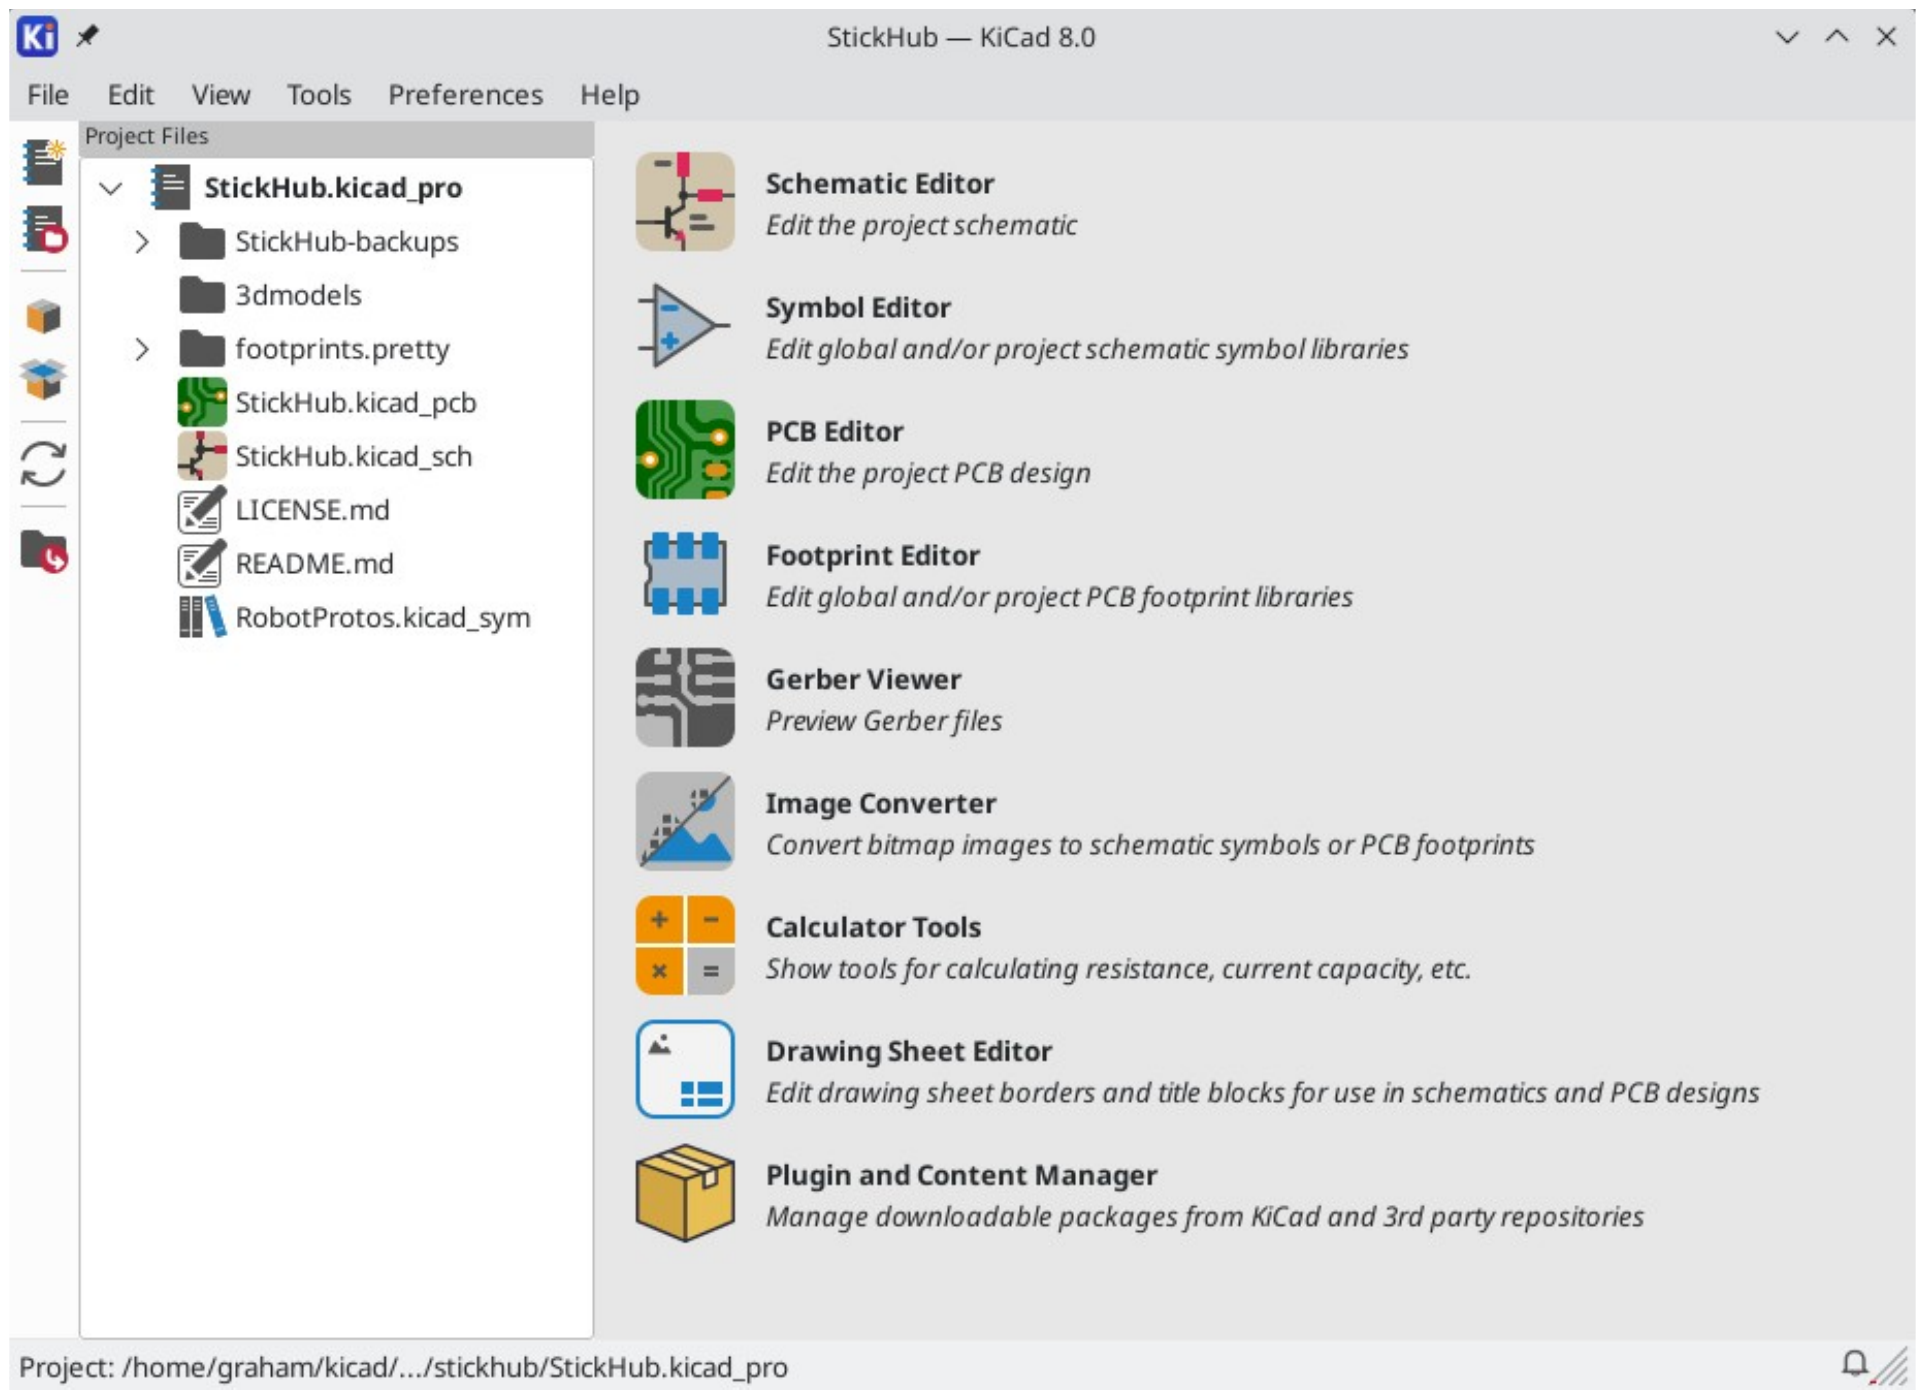
\includegraphics[max width=\linewidth,max height=0.82\textheight]{figuras/figura-22.png}
\label{fig:22}
\caption{Figura 22: Gerenciador de Projetos. Fonte: \url{https://docs.kicad.org/8.0/en/kicad/kicad.html\#:~:text=Usando\%20o} \%20gerenciador,editores\%20e\%20ferramentas}
\end{figure}

A janela do gerenciador de projetos do KiCad é composta por uma visualização em árvore à esquerda, mostrando os arquivos associados ao projeto aberto, e um iniciador à direita, contendo atalhos para os vários editores e ferramentas.

\hypertarget{arquivos-e-pastas-kicad}{%
\section{Arquivos e pastas KiCad}\label{arquivos-e-pastas-kicad}}

O KiCad cria e usa arquivos com as seguintes extensões de arquivo (e pastas) específicas para edição de esquemas e placas.

\hypertarget{arquivos-de-projeto}{%
\subsection{Arquivos de projeto}\label{arquivos-de-projeto}}

Arquivo de projeto, contendo configurações que são compartilhadas *.kicad\_pro entre o esquema e o PCB

*.pro Arquivo de projeto Legacy (KiCad 5.x e anterior). Pode ser lido e será

convertido em um.kicad\_proarquivo pelo gerente de projeto.

\hypertarget{arquivos-do-editor-esquemuxe1tico}{%
\subsubsection{Arquivos do editor esquemático}\label{arquivos-do-editor-esquemuxe1tico}}

Arquivos esquemáticos contendo todas as informações e os próprios *.kicad\_sch componentes.

Arquivo de biblioteca de símbolos esquemáticos, contendo as *.kicad\_sym descrições dos componentes: forma gráfica, pinos, campos.

Arquivo esquemático legado (KiCad 5.x e anterior). Pode ser lido e *.sch será convertido em um.kicad\_scharquivo na gravação.

Arquivo de biblioteca esquemática Legacy (KiCad 5.x e anteriores). *.lib Pode ser lido, mas não escrito.

Documentação da biblioteca esquemática legada (KiCad 5.x e *.dcm anterior). Pode ser lida, mas não escrita.

Arquivo de cache de biblioteca de componentes esquemáticos legados *-cache.lib (KiCad 5.x e anteriores). Necessário para o carregamento adequado de um.scharquivo esquemático legado ( ).

Tabela de biblioteca de símbolos: sym-lib-table, lista de bibliotecas de símbolos disponíveis no editor de esquemáticos.

\hypertarget{arquivos-e-pastas-do-editor-de-pcb}{%
\subsubsection{Arquivos e pastas do editor de PCB}\label{arquivos-e-pastas-do-editor-de-pcb}}

Arquivo do quadro contendo todas as informações, exceto o layout da *.kicad\_pcb página.

*.pretty Pastas da biblioteca Footprint. A pasta em si é a biblioteca.

*.kicad\_mod Arquivos de pegada, contendo uma descrição de pegada cada.

Arquivo de regras de design, contendo regras de design *.kicad\_dru personalizadas para um.kicad\_pcbarquivo específico.

Arquivo de placa Legacy (KiCad 4.x e anteriores). Pode ser lido, mas *.brd não escrito, pelo editor de placa atual.

\begingroup\scriptsize\begin{longtable}[]{@{}
  >{\raggedright\arraybackslash}p{(\columnwidth - 2\tabcolsep) * \real{0.5000}}
  >{\raggedright\arraybackslash}p{(\columnwidth - 2\tabcolsep) * \real{0.5000}}@{}}
\toprule\noalign{}
\begin{minipage}[b]{\linewidth}\raggedright
*.mod fp-lib-table fp-info-cache
\end{minipage} & \begin{minipage}[b]{\linewidth}\raggedright
Arquivo de biblioteca de footprint legado (KiCad 4.x e anterior). Pode ser lido pelo footprint ou pelo editor de placa, mas não escrito. Tabela de biblioteca de footprint: lista de bibliotecas de footprint disponíveis no editor de quadro. Cache para acelerar o carregamento de bibliotecas de footprint. Não precisa ser distribuído com o projeto ou colocado sob controle de versão.
\end{minipage} \\
\midrule\noalign{}
\endhead
\bottomrule\noalign{}
\endlastfoot
& Arquivos comuns \\
*.kicad\_prl & Configurações locais para o projeto atual; ajuda o KiCad a lembrar as últimas configurações usadas, como visibilidade de camada ou filtro de seleção. Pode não precisar ser distribuído com o projeto ou colocado sob controle de versão. \\
*.kicad\_wks & Arquivo de descrição do layout da página (borda do desenho e bloco de título) \\
\emph{.net }.cmp & Arquivo netlist criado a partir do esquema e lido pelo editor de placa. Observe que o fluxo de trabalho recomendado para transferir informações do esquema para a placa não requer o uso de arquivos netlist. Associação entre componentes usados no esquemático e seus footprints. Pode ser criado pelo Board Editor e importado pelo Schematic Editor. Seu propósito é importar alterações do board para o esquemático, para usuários que alteram footprints no Board Editor (por exemplo, usando o comando Exchange Footprints) e querem importar essas alterações de volta para o esquemático. Observe que o fluxo de trabalho recomendado para transferir informações do board para o esquemático não requer o uso de.cmparquivos. Instituto Federal Fluminense 36 \\
\end{longtable}\endgroup

\hypertarget{arquivos-de-fabricauxe7uxe3o-e-documentauxe7uxe3o}{%
\subsubsection{Arquivos de fabricação e documentação}\label{arquivos-de-fabricauxe7uxe3o-e-documentauxe7uxe3o}}

\begingroup\scriptsize\begin{longtable}[]{@{}
  >{\raggedright\arraybackslash}p{(\columnwidth - 2\tabcolsep) * \real{0.5000}}
  >{\raggedright\arraybackslash}p{(\columnwidth - 2\tabcolsep) * \real{0.5000}}@{}}
\toprule\noalign{}
\begin{minipage}[b]{\linewidth}\raggedright
*.gbr
\end{minipage} & \begin{minipage}[b]{\linewidth}\raggedright
Arquivo Gerber, para fabricação.
\end{minipage} \\
\midrule\noalign{}
\endhead
\bottomrule\noalign{}
\endlastfoot
*.drl & Arquivo de perfuração (formato Excellon), para fabricação. \\
*.pos & Arquivos de posição (formato ASCII), para máquinas de inserção automática. \\
*.rpt & Arquivos de relatório (formato ASCII), para documentação. \\
*.ps & Arquivos de plotagem (Postscript), para documentação. \\
*.pdf & Arquivos de plotagem (formato PDF), para documentação. \\
*.svg & Arquivos de plotagem (formato SVG), para documentação. \\
*.dxf & Arquivos de plotagem (formato DXF), para documentação. \\
\end{longtable}\endgroup

*.plt Arquivos de plotagem (formato HPGL), para documentação.

\hypertarget{armazenando-e-enviando-arquivos-kicad}{%
\subsection{Armazenando e enviando arquivos KiCad}\label{armazenando-e-enviando-arquivos-kicad}}

Os arquivos de esquema e placa do KiCad contêm todos os símbolos esquemáticos e footprints usados no design, então você pode fazer backup ou enviar esses arquivos por si só sem problemas. Algumas informações importantes do design são armazenadas no arquivo do projeto (.kicad\_pro), então se você estiver enviando um design completo, certifique-se de incluí-lo. Alguns arquivos, como o arquivo project-local settings (.kicad\_prl) e o arquivo fp-info-cache, não são necessários para enviar com seu projeto. Se você usa um sistema de controle de versão como o Git para manter o controle de seus projetos KiCad, você pode querer adicionar esses arquivos à lista de arquivos ignorados para que eles não sejam rastreados. Outros detalhes inclusive de configurações pode ser obtidos em:

\url{https://docs.kicad.org/8.0/en/kicad/kicad.html}

\hypertarget{workflow-do-kicad}{%
\section{Workflow do Kicad}\label{workflow-do-kicad}}

O fluxo de trabalho (workflow) do KiCad geralmente segue as etapas comuns de projeto de circuitos eletrônicos e design de PCB. Entretanto, conforme o desejo do projetista, algumas etapas do workflow podem ser alteradas ou até suprimidas durante o design. Ver exemplo na figura.

\begin{figure}[H]
\centering
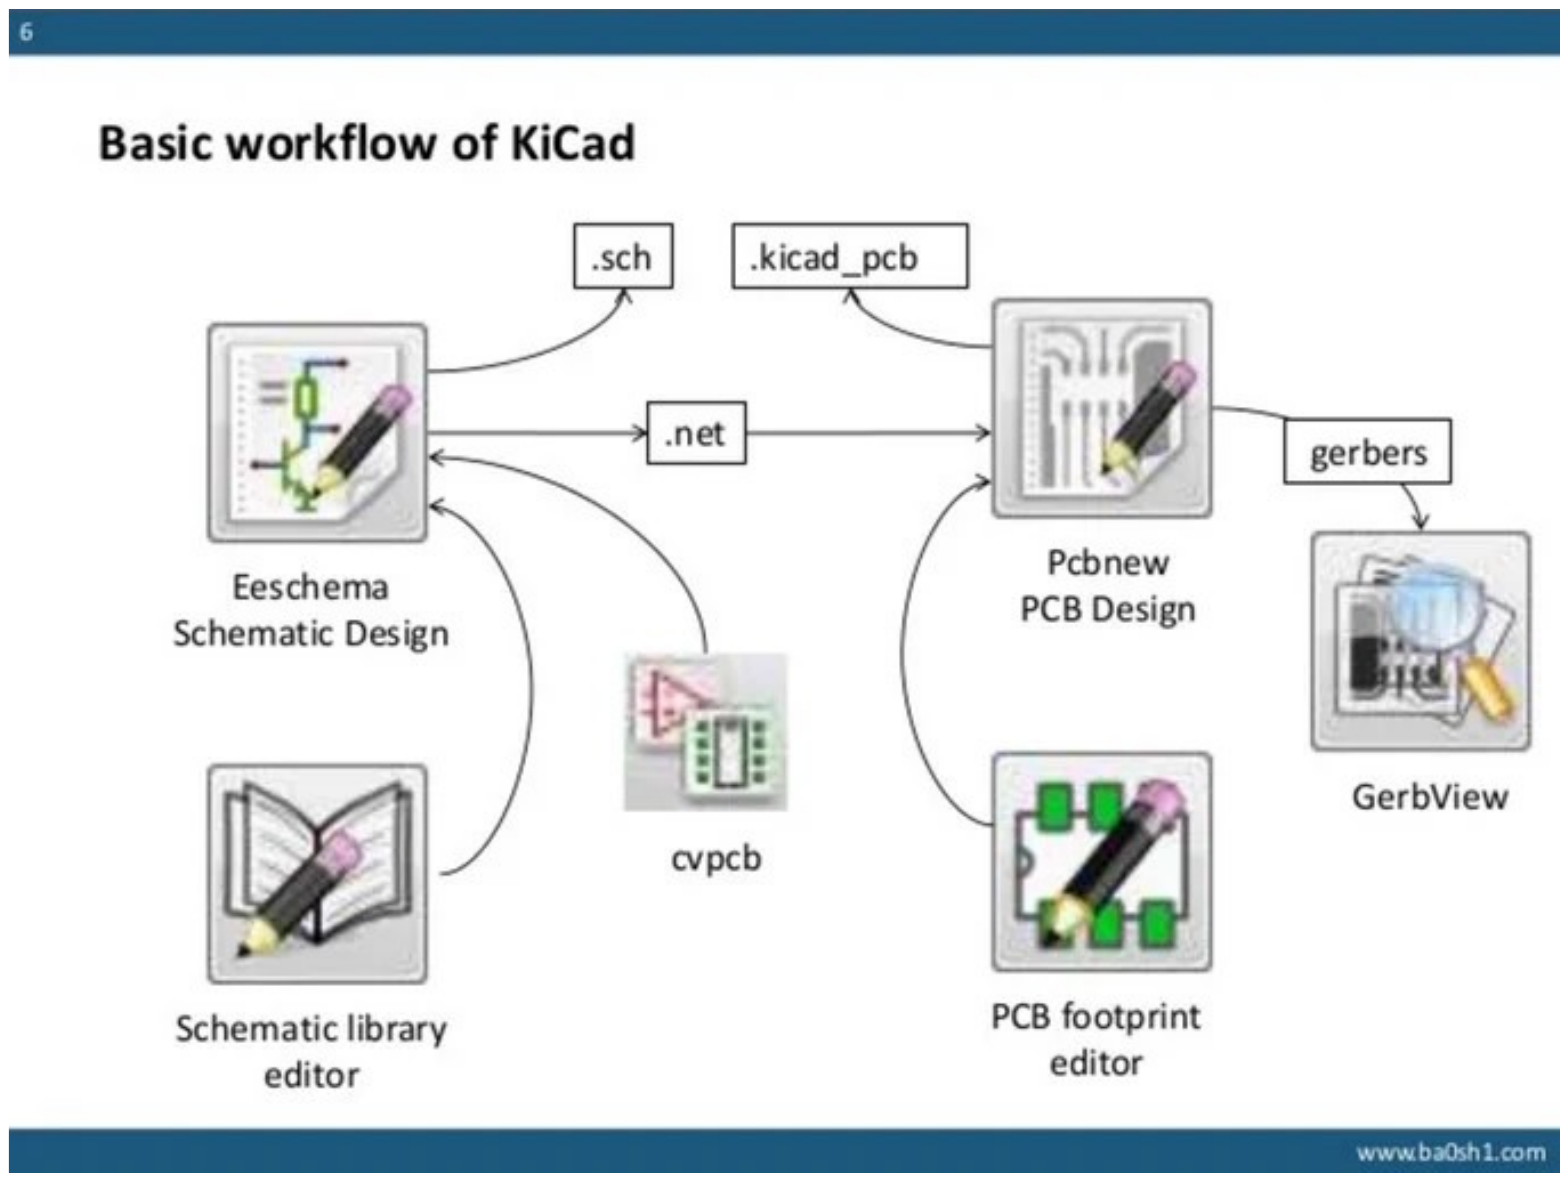
\includegraphics[max width=\linewidth,max height=0.82\textheight]{figuras/figura-23.png}
\label{fig:23}
\caption{Figura 23: Workflow básico KiCAD. fonte: \url{https://www.slideshare.net/baoshi1/why-} and-how-to-switch-to-kicad}
\end{figure}

Abaixo estão as principais etapas do workflow do KiCad:

\hypertarget{esquemuxe1tico-schematic}{%
\subsection{Esquemático (Schematic):}\label{esquemuxe1tico-schematic}}

\begin{itemize}
\item
  Crie um novo projeto no KiCad.
\item
  Configure a página e esquemático.
\item
  Desenhe o esquemático do circuito eletrônico usando o editor esquemático do KiCad.
\item
  Adicione componentes eletrônicos ao esquemático, selecionando-os a partir da biblioteca de componentes ou criando novos componentes, se necessário.
\item
  Conecte os componentes eletrônicos usando os símbolos de fios ou barramentos.
\item
  Preencha os designadores dos componentes eletrônicos
\end{itemize}

\hypertarget{associauxe7uxe3o-de-footprints-assigning-footprints}{%
\subsection{Associação de Footprints (Assigning Footprints):}\label{associauxe7uxe3o-de-footprints-assigning-footprints}}

\begin{itemize}
\tightlist
\item
  Após finalizar o esquemático, associe os componentes com suas respectivas footprints no layout da PCB. O footprint é a representação física do componente na placa de circuito impresso.
\end{itemize}

\hypertarget{layout-da-pcb-pcb-layout}{%
\subsection{Layout da PCB (PCB Layout):}\label{layout-da-pcb-pcb-layout}}

\begin{itemize}
\tightlist
\item
  Abra o editor de PCB e importe o netlist do esquemático para criar o layout da placa de circuito impresso (PCB).
\item
  Posicione os componentes na placa e organize-os de acordo com suas preferências e requisitos de design.
\item
  Trace as trilhas de cobre para conectar os componentes eletrônicos corretamente.
\item
  Realize o roteamento das trilhas de forma a evitar cruzamentos indesejados e garantir o melhor desempenho do circuito.
\end{itemize}

\hypertarget{visualizauxe7uxe3o-3d-3d-visualization}{%
\subsection{Visualização 3D (3D Visualization):}\label{visualizauxe7uxe3o-3d-3d-visualization}}

\begin{itemize}
\tightlist
\item
  Utilize a visualização 3D do KiCad para verificar a colocação dos componentes na PCB e garantir que não haja interferências ou problemas de montagem.
\end{itemize}

\hypertarget{verificauxe7uxe3o-do-design-design-verification}{%
\subsection{Verificação do Design (Design Verification):}\label{verificauxe7uxe3o-do-design-design-verification}}

\begin{itemize}
\tightlist
\item
  Realize uma revisão completa do projeto, verificando a conformidade das trilhas, a ausência de erros de conexão, e garantindo que todas as regras de projeto estejam sendo seguidas.
\end{itemize}

\hypertarget{gerauxe7uxe3o-dos-arquivos-de-fabricauxe7uxe3o-manufacturing-files}{%
\subsection{Geração dos Arquivos de Fabricação (Manufacturing Files):}\label{gerauxe7uxe3o-dos-arquivos-de-fabricauxe7uxe3o-manufacturing-files}}

\begin{itemize}
\tightlist
\item
  Após concluir o design da PCB, gere os arquivos necessários para a fabricação da placa, incluindo Gerber files, Drill files, entre outros.
\end{itemize}

\hypertarget{importauxe7uxe3o-e-utilizauxe7uxe3o-de-bibliotecas-de-componentes-no-kicad}{%
\section{Importação e utilização de bibliotecas de componentes no KiCad}\label{importauxe7uxe3o-e-utilizauxe7uxe3o-de-bibliotecas-de-componentes-no-kicad}}

O KiCad possui várias bibliotecas de componentes, mas existem outras disponíveis online.

\hypertarget{as-bibliotecas-suxe3o}{%
\subsubsection{As bibliotecas são:}\label{as-bibliotecas-suxe3o}}

\begin{itemize}
\tightlist
\item
  symbols → símbolos utilizados no editor de esquemático do KiCad
\item
  footprints → footprints utilizados no editor da PCB
\item
  packages3D → modelos 3D utilizados na renderização feita no visualizador da PCB
  \par\noindent\makebox[\linewidth][c]{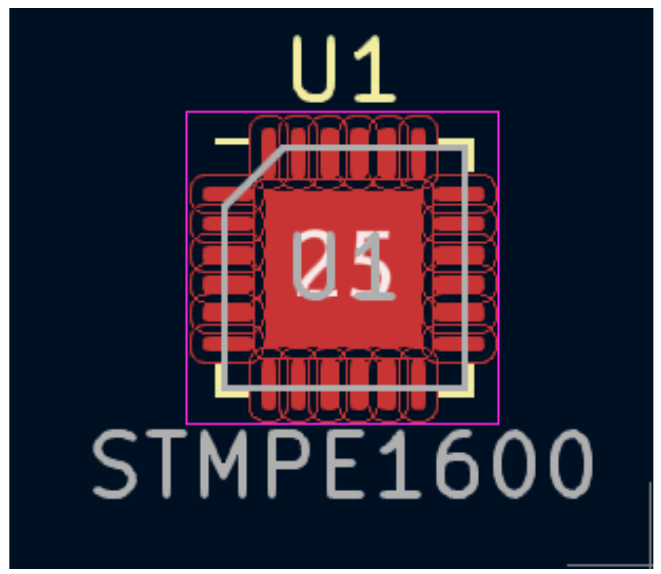
\includegraphics[max width=\linewidth,max height=0.82\textheight]{figuras/figura-25.png}}\par\label{fig:25}
\end{itemize}

\begin{figure}[H]
\centering
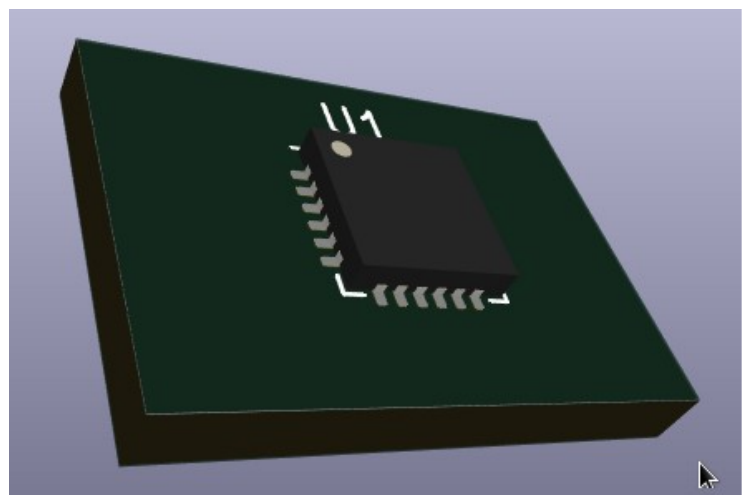
\includegraphics[max width=\linewidth,max height=0.82\textheight]{figuras/figura-26.png}
\label{fig:26}
\caption{Figura 26: Exemplo de modelos 3D}
\end{figure}

\begin{figure}[H]
\centering
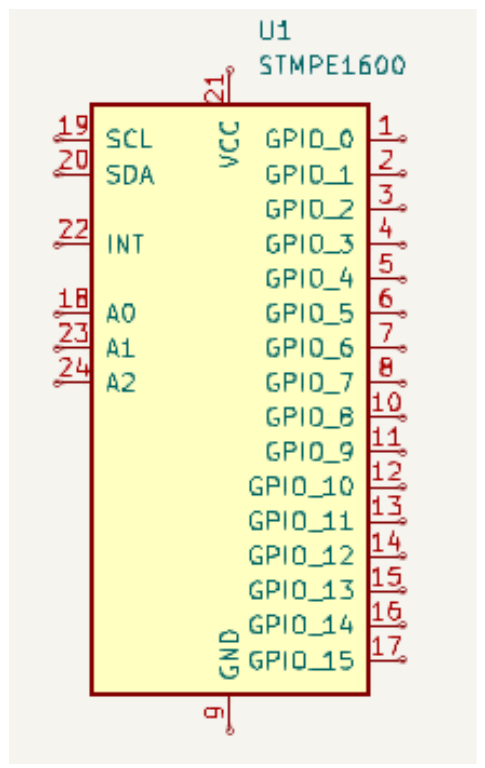
\includegraphics[max width=\linewidth,max height=0.82\textheight]{figuras/figura-24.png}
\label{fig:24}
\caption{Figura 24: Exemplo de símbolo}
\end{figure}

\hypertarget{utilizauxe7uxe3o-de-novas-bibliotecas}{%
\subsection{Utilização de novas bibliotecas}\label{utilizauxe7uxe3o-de-novas-bibliotecas}}

As seguintes bibliotecas são as oficiais:

\url{https://gitlab.com/kicad/libraries/kicad-symbols}

\url{https://gitlab.com/kicad/libraries/kicad-footprints}

\url{https://gitlab.com/kicad/libraries/kicad-packages3D}

\url{https://gitlab.com/kicad/libraries/kicad-packages3D-source}

\url{https://gitlab.com/kicad/libraries/kicad-templates}

Entretanto, existem outras fontes on-line que podem ser utilizadas para obtenção de bibliotecas. Exemplos:

\url{https://www.ultralibrarian.com/}

\url{https://www.snapeda.com/}

Também pode-se encontrar bibliotecas específicas de fabricantes, ou ainda, é possível criar seus próprios símbolos, footprints e modelos 3D.

O plugin que aumenta a produtividade é o easyeda2kicad.

O projeto com instruções pode ser acessado pela url: \url{https://pypi.org/project/easyeda2kicad/}

No Linux ou Windows é possível instalar a partir dos comandos:

\begin{verbatim}
python3 -m venv kicadlib
\end{verbatim}

\textbf{\emph{source kicadlib/bin/activate}}

\begin{verbatim}
pip install easyeda2kicad

easyeda2kicad --full –lcsc_id=C2040
\end{verbatim}

Onde C2040 pode ser substituído pelo id do componente disponível em

\url{https://jlcpcb.com/PARTS}

Por exemplo: pretende-se incluir no Kicad as bibliotecas do componente ATGM336H-5N31.

\begin{figure}[H]
\centering
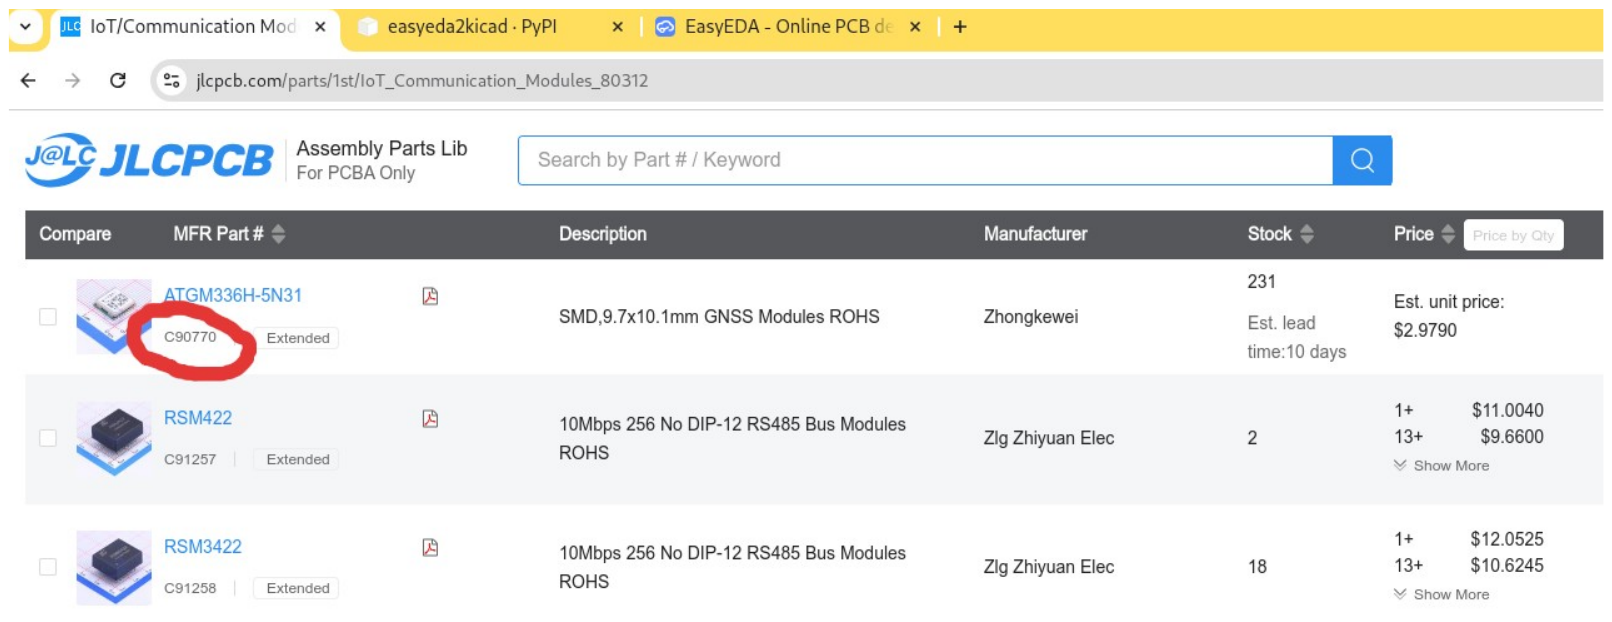
\includegraphics[max width=\linewidth,max height=0.82\textheight]{figuras/figura-27.png}
\label{fig:27}
\caption{Figura 27: Exemplo de indentificação do Part na JLCPCB}
\end{figure}

Então digite o comando:

\begin{verbatim}
easyeda2kicad --full –lcsc_id=C90770
\end{verbatim}

Símbolo, Footprint e modelo 3D serão baixados para o seu PC em diretório padrão, mas é possível especificar o diretório de destino.

\begin{verbatim}
easyeda2kicad --full --lcsc_id=C2040 --output ~/libs/my_lib
\end{verbatim}

No KiCad, vá em Preferências \textgreater{} Configurar Caminhos e adicione as variáveis de ambiente EASYEDA2KICAD:

\begin{verbatim}
Windows : C:/Users/your_username/Documents/Kicad/easyeda2kicad/,

Linux:/home/your_username/libs
\end{verbatim}

Vá para Preferências \textgreater{} Gerenciar Bibliotecas de Símbolos e Adicione a biblioteca global

\textbf{easyeda2kicad:\$\{EASYEDA2KICAD\}/my\_lib.kicad\_sym}

Vá para Preferências \textgreater{} Gerenciar bibliotecas do Footprint e adicione a biblioteca global

\textbf{easyeda2kicad:\$\{EASYEDA2KICAD\}/my\_lib.pretty}

Nesse caso o componente já estará com o campo ``LCSC Part'' contendo o código exato que fará parte da lista BOM (veja a figura).

\begin{figure}[H]
\centering
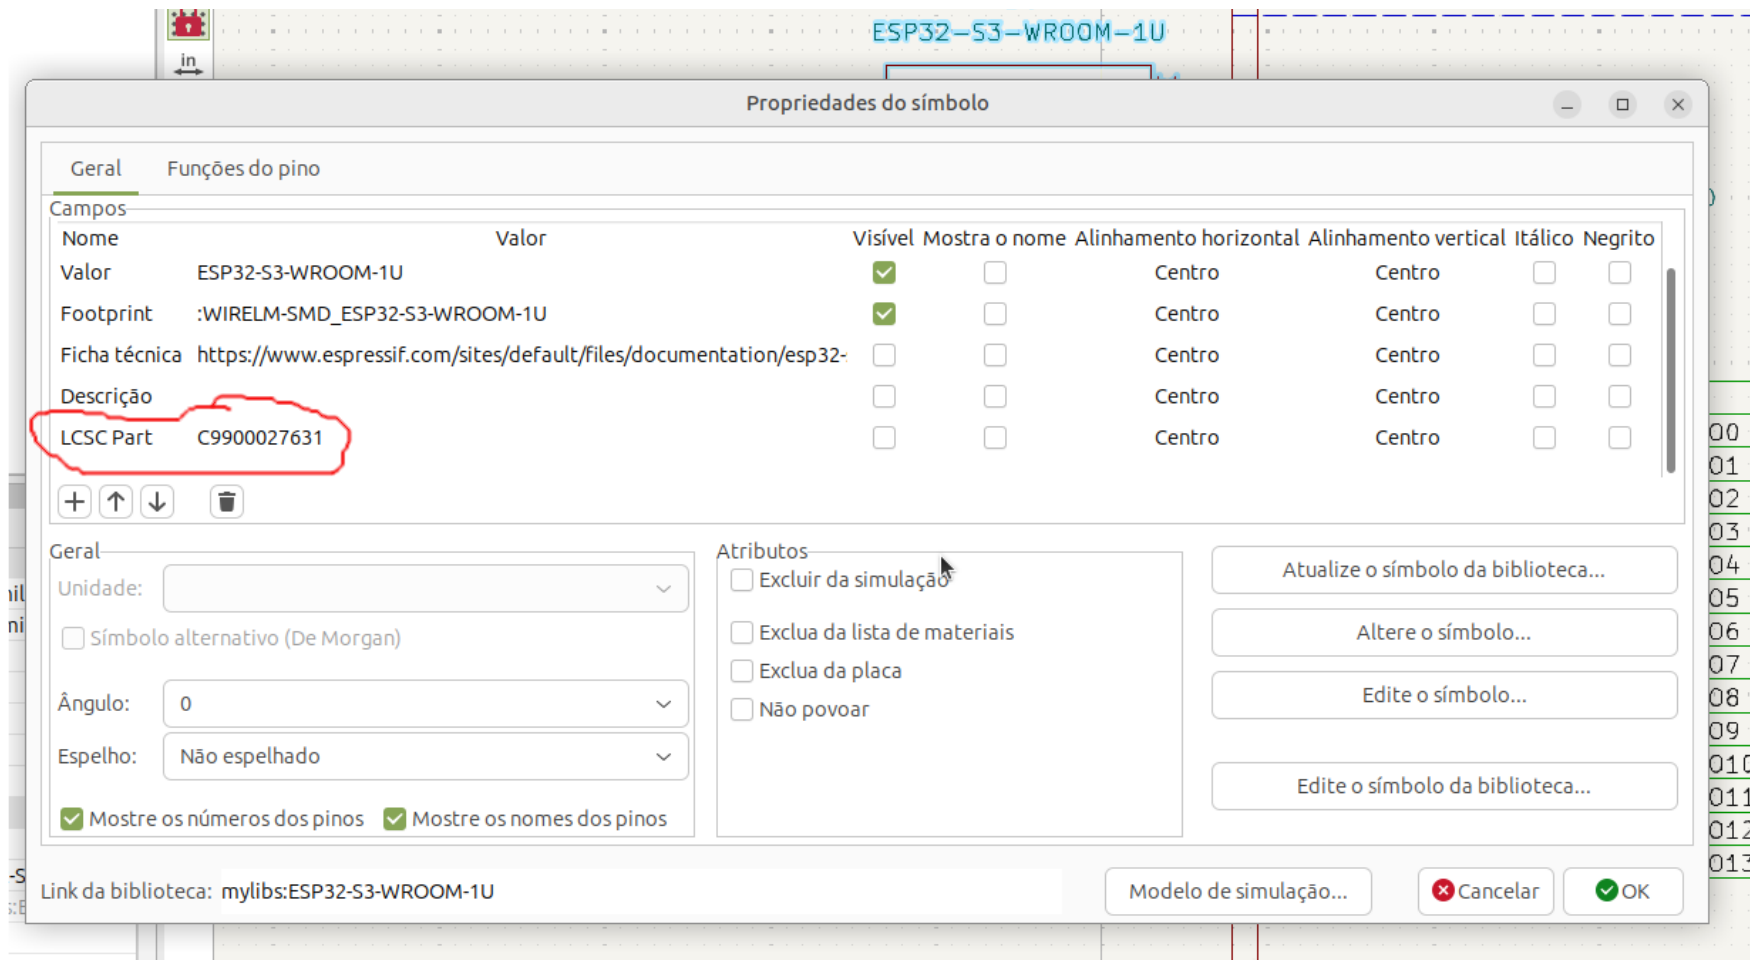
\includegraphics[max width=\linewidth,max height=0.82\textheight]{figuras/figura-28.png}
\label{fig:28}
\caption{Figura 28: Identificação do componente a ser utilizado na lista BOM para fabricação na JLCPCB}
\end{figure}

\begin{figure}[H]
\centering
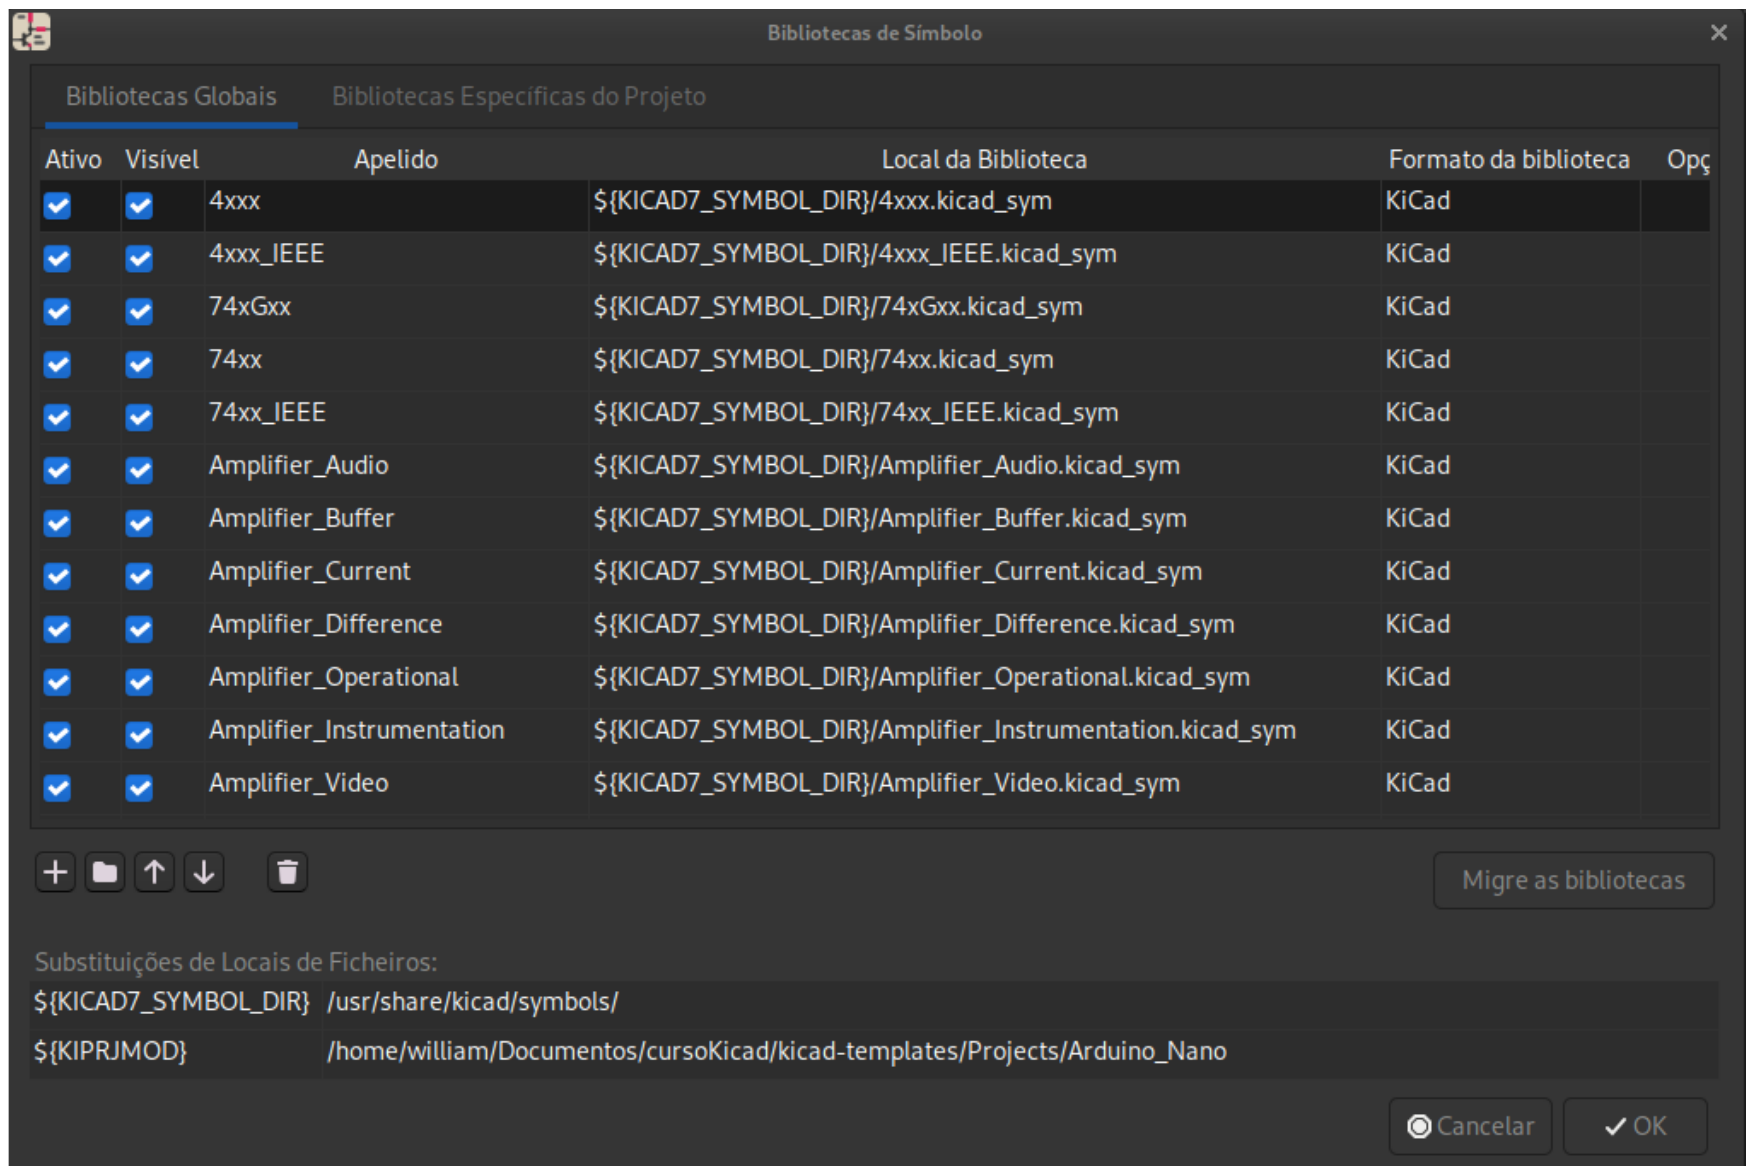
\includegraphics[max width=\linewidth,max height=0.82\textheight]{figuras/figura-29.png}
\label{fig:29}
\caption{Figura 29: Configuração das bibliotecas de símbolos}
\end{figure}

Caso as biblioteca seja específica do projeto e altamente recomendável que esteja em um diretório do projeto.

Caso deseje incluir as bibliotecas apenas no projeto e dentro dos respectivos diretórios do mesmo, use o caminho da seguinte forma:

\begin{verbatim}
${KIPRJMOD}/libs/my_libs.kicad_sym
\end{verbatim}

\hypertarget{principais-teclas-de-atalho}{%
\section{Principais teclas de atalho}\label{principais-teclas-de-atalho}}

\hypertarget{editor-de-esquemuxe1ticos-eeschema}{%
\subsection{Editor de Esquemáticos (Eeschema)}\label{editor-de-esquemuxe1ticos-eeschema}}

\begingroup\scriptsize\begin{longtable}[]{@{}
  >{\raggedright\arraybackslash}p{(\columnwidth - 2\tabcolsep) * \real{0.5000}}
  >{\raggedright\arraybackslash}p{(\columnwidth - 2\tabcolsep) * \real{0.5000}}@{}}
\toprule\noalign{}
\begin{minipage}[b]{\linewidth}\raggedright
Tecla de Atalho
\end{minipage} & \begin{minipage}[b]{\linewidth}\raggedright
Descrição
\end{minipage} \\
\midrule\noalign{}
\endhead
\bottomrule\noalign{}
\endlastfoot
A & Adicionar um novo componente ao esquemático. \\
M & Mover o componente selecionado. \\
G & Mover o componente sem desconectar as conexões. \\
R & Girar o componente selecionado (90° no sentido horário). \\
Ctrl + R & Girar no sentido anti-horário. \\
X & Adicionar um fio elétrico. \\
Shift + X & Adicionar um fio de barramento. \\
L & Adicionar uma etiqueta do fio (Label). \\
Ctrl + B & Alternar exibição de nomes de barramento e rótulos. \\
F5, F6, F7, F8 & Alternar entre diferentes folhas do projeto hierárquico. \\
Ctrl + E & Editar o componente selecionado. \\
Ctrl + Shift + E & Editar as propriedades do componente. \\
Delete & Excluir o item selecionado. \\
Ctrl + Z & Desfazer a última ação. \\
Ctrl + Y & Refazer a última ação desfeita. \\
Ctrl + F & Localizar componentes ou rótulos. \\
Ctrl + G & Gerar netlist (rede elétrica). \\
\end{longtable}\endgroup

\hypertarget{editor-de-pcb-pcbnew}{%
\subsection{Editor de PCB (Pcbnew)}\label{editor-de-pcb-pcbnew}}

\begingroup\scriptsize\begin{longtable}[]{@{}
  >{\raggedright\arraybackslash}p{(\columnwidth - 2\tabcolsep) * \real{0.5000}}
  >{\raggedright\arraybackslash}p{(\columnwidth - 2\tabcolsep) * \real{0.5000}}@{}}
\toprule\noalign{}
\begin{minipage}[b]{\linewidth}\raggedright
Tecla de Atalho
\end{minipage} & \begin{minipage}[b]{\linewidth}\raggedright
Descrição
\end{minipage} \\
\midrule\noalign{}
\endhead
\bottomrule\noalign{}
\endlastfoot
A & Adicionar um componente à PCB. \\
M & Mover o componente selecionado. \\
G & Mover o componente mantendo as conexões (empurrar e ajustar). \\
R & Rotacionar o componente selecionado. \\
Ctrl + R & Rotacionar no sentido anti-horário. \\
F & Alternar entre os lados da PCB (superior/inferior). \\
Ctrl + H & Alternar exibição de vias e trilhas invisíveis. \\
X & Adicionar uma trilha. \\
V & Adicionar uma via. \\
Shift + X & Entra no modo de ``Roteamento'' para adicionar trilhas conectadas. \\
Ctrl + Shift + B & Atualizar os componentes da PCB com base no esquemático. \\
Ctrl + Z & Desfazer a última ação. \\
Ctrl + Y & Refazer a última ação desfeita. \\
Delete & Excluir o item selecionado. \\
Ctrl + Alt + V & Adicionar trilha em via (Jump). \\
Ctrl + F & Localizar componentes na PCB. \\
Ctrl + Shift + D & Alterar as dimensões do contorno da PCB. \\
Ctrl + M & Medir distâncias entre dois pontos. \\
\end{longtable}\endgroup

\hypertarget{teclas-globais}{%
\subsection{Teclas Globais}\label{teclas-globais}}

Estas teclas funcionam em ambos os editores:

\hypertarget{tecla-de}{%
\subsubsection{Tecla de}\label{tecla-de}}

\hypertarget{descriuxe7uxe3o}{%
\subsubsection{Descrição}\label{descriuxe7uxe3o}}

\hypertarget{atalho}{%
\subsubsection{Atalho}\label{atalho}}

\begingroup\scriptsize\begin{longtable}[]{@{}ll@{}}
\toprule\noalign{}
Ctrl + S & Salvar o projeto. \\
\midrule\noalign{}
\endhead
\bottomrule\noalign{}
\endlastfoot
Ctrl + O & Abrir um projeto existente. \\
Ctrl + N & Criar um novo projeto. \\
Ctrl + P & Imprimir o projeto atual. \\
\end{longtable}\endgroup

\hypertarget{tecla-de-1}{%
\subsubsection{Tecla de}\label{tecla-de-1}}

\hypertarget{descriuxe7uxe3o-1}{%
\subsubsection{Descrição}\label{descriuxe7uxe3o-1}}

\hypertarget{atalho-1}{%
\subsubsection{Atalho}\label{atalho-1}}

\textbf{F11} Alternar para modo tela cheia. Acessar o menu de ajuda/documentação do \textbf{F1} KiCad.

Essas teclas de atalho são padrão no KiCad 8 e podem ser ajustadas em \textbf{Preferências \textgreater{} Configuração de Atalhos} caso você precise personalizá-las.

\hypertarget{compatibilidade-do-design-da-pcb-para-fabricauxe7uxe3o}{%
\section{Compatibilidade do Design da PCB para fabricação}\label{compatibilidade-do-design-da-pcb-para-fabricauxe7uxe3o}}

As empresas que realizam a manufatura das PCBs de forma comercial possuem limites técnicos que por vezes impossibilitam a fabricação caso o projetista não esteja atendo aos limites imposto pelo fabricante. Nesse caso é muito importante consultar os parâmetros definidos pelo fabricante e inseri-los nas no verificados de regras da PCB.

As configurações de restrição podem ser inseridas no KiCAD ``Configuração da Placa → Regras de Desenho → Restrições''. Ver figura.

\begin{quadro}{green!50!black}{Antes de mandar fabricar}
Insira no KiCAD as restrições técnicas de fabricação, para que o próprio
KiCAD aponte inconsistências no projeto, e trabalhe com \textbf{margem
de pelo menos 20\%} em relação aos limites do fabricante.

\textbf{Nota:} a estrutura desta tabela foi corrompida na conversão
(células desalinhadas). Os valores precisam ser conferidos na página do
fabricante antes do uso --- a revisão está pendente.
\end{quadro}

\begin{figure}[H]
\centering
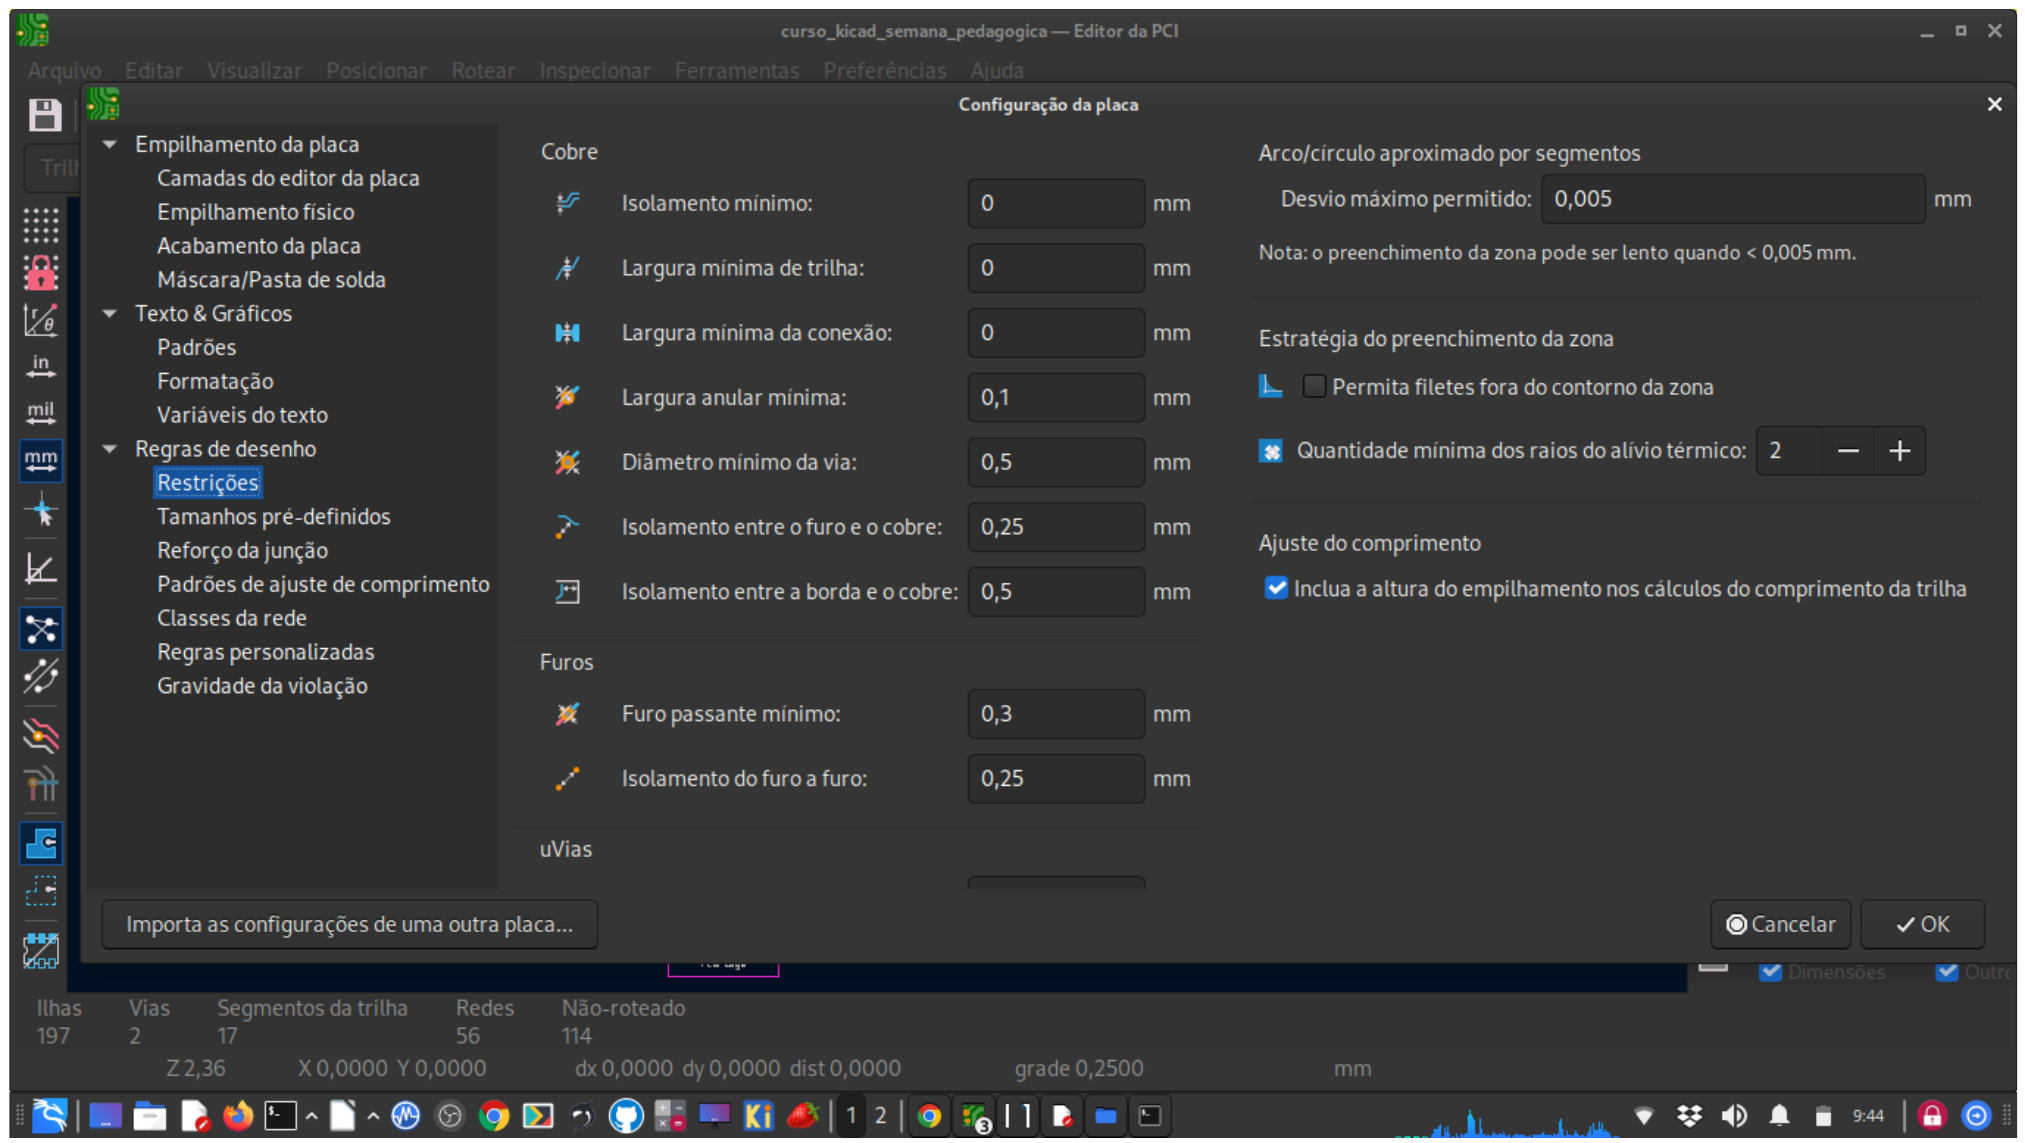
\includegraphics[max width=\linewidth,max height=0.82\textheight]{figuras/figura-30.png}
\label{fig:30}
\caption{Figura 30: Interface de configuração das restrições de desenho da PCB}
\end{figure}

As compatibilidades apresentadas foram conferidas na JLCPCB em 09/2026, a partir da url \href{https://jlcpcb.com/capabilities/pcb-capabilities}{jlcpcb.com/capabilities/pcb-capabilities}. Os valores são os publicados pelo fabricante nessa data e mudam com o tempo --- confira a página antes de usar.

\hypertarget{especificauxe7uxf5es-do-pcb}{%
\subsubsection{Especificações do PCB}\label{especificauxe7uxf5es-do-pcb}}

\begingroup\scriptsize\begin{longtable}[]{@{}
  >{\raggedright\arraybackslash}p{(\columnwidth - 4\tabcolsep) * \real{0.3333}}
  >{\raggedright\arraybackslash}p{(\columnwidth - 4\tabcolsep) * \real{0.3333}}
  >{\raggedright\arraybackslash}p{(\columnwidth - 4\tabcolsep) * \real{0.3333}}@{}}
\toprule\noalign{}
\begin{minipage}[b]{\linewidth}\raggedright
Característica
\end{minipage} & \begin{minipage}[b]{\linewidth}\raggedright
Capacidade
\end{minipage} & \begin{minipage}[b]{\linewidth}\raggedright
Descrição
\end{minipage} \\
\midrule\noalign{}
\endhead
\bottomrule\noalign{}
\endlastfoot
Contagem de camadas & 1--32 & Número de camadas de cobre da placa. \\
Impedância controlada & 4/6/8/10/12/14/16/18/20/\ldots/32 camadas & Ver a calculadora de impedância da JLCPCB. \\
Tolerância de impedância & ±10\% & Tolerância padrão do serviço; ±5\% sob consulta. \\
Material & FR-4 & Laminados grau A de fornecedores como Nan Ya, KB e Shengyi. \\
HDI & 1-step / 2-step / 3-step & Via cega de 0,075--0,15 mm (perfuração a laser); via enterrada de 0,15--0,55 mm padrão e até 0,10 mm em casos extremos; trilha/espaço mínimo de 3/3 mil (2,7/2,7 mil extremo); dimensões de 5 × 5 mm a 576 × 469 mm. \\
Núcleo de alumínio & 1 camada & PCBs de núcleo de alumínio de uma camada. \\
Núcleo de cobre & 1 camada & PCBs de núcleo de cobre de uma camada, com contato direto do dissipador ao núcleo (≥ 1 × 1 mm). \\
PCB de RF & 2 camadas, 1 oz & Núcleos de Rogers e PTFE. \\
Constantes dielétricas do FR-4 & 4,5 (placa de 2 camadas) & Prepreg 7628: 4,4; 3313: 4,1; 2116: 4,16. \\
Dimensões máximas & FR-4 (1 camada): 606 × 510 mm; FR-4 (2 camadas): 670 × 600 mm; FR-4 (4 camadas): 663 × 593 mm; FR-4 (6+ camadas): 656 × 586 mm; Rogers/PTFE: 590 × 438 mm; alumínio: 602 × 506 mm; cobre: 480 × 286 mm & Válido para placas com espessura ≥ 0,8 mm; FR-4 mais fino chega a 599 × 497 mm. Placas de 2 camadas podem atingir 1020 × 600 mm e as de 4 camadas, 1016 × 596 mm. \\
Dimensões mínimas & FR-4/Rogers/PTFE: 3 × 3 mm; bordas chapeadas ou casteladas: 10 × 10 mm; alumínio/cobre: 5 × 5 mm & Válido para espessuras ≥ 0,6 mm; abaixo disso exige revisão manual. A painelização é recomendada para placas pequenas. \\
Tolerância dimensional & ±0,1 mm & ±0,1 mm (precisão) e ±0,2 mm (regular) no roteamento CNC; ±0,4 mm no corte em V. \\
Espessura & 0,4--4,5 mm & FR-4 em 0,4/0,6/0,8/1,0/1,2/1,6/2,0 mm (2,5 mm ou mais apenas para placas de 12 camadas ou mais). \\
Tolerância de espessura (≥ 1,0 mm) & ±10\% & Ex.: placa de 1,6 mm → acabada entre 1,44 mm e 1,76 mm. \\
Tolerância de espessura (\textless{} 1,0 mm) & ±0,1 mm & Ex.: placa de 0,8 mm → acabada entre 0,7 mm e 0,9 mm. \\
Cobre acabado --- camada externa & 2 camadas: 1/2/2,5/3,5/4,5 oz; multicamadas: 1/2 oz & --- \\
Cobre acabado --- camada interna & 0,5/1/2 oz & 0,5 oz por padrão na camada interna. \\
Máscara de solda & Verde, roxo, vermelho, amarelo, azul, branco e preto & Máscara LPI (\emph{Liquid Photo Imageable}), a mais comum. A de tinta curada a calor aparece em placas de baixo custo e de um lado só. \\
Acabamento de superfície & HASL (com e sem chumbo), ENIG, OSP & OSP não está disponível para FR-4 de face única, FPC e placas de alumínio; placas de alumínio aceitam apenas HASL. FR-4/HDI com 6 camadas ou mais, espessura ≤ 0,4 mm, alta frequência, núcleo de cobre e FPC não suportam HASL. \\
\end{longtable}\endgroup

\hypertarget{perfurauxe7uxe3o}{%
\subsubsection{Perfuração}\label{perfurauxe7uxe3o}}

\begingroup\scriptsize\begin{longtable}[]{@{}
  >{\raggedright\arraybackslash}p{(\columnwidth - 4\tabcolsep) * \real{0.3333}}
  >{\raggedright\arraybackslash}p{(\columnwidth - 4\tabcolsep) * \real{0.3333}}
  >{\raggedright\arraybackslash}p{(\columnwidth - 4\tabcolsep) * \real{0.3333}}@{}}
\toprule\noalign{}
\begin{minipage}[b]{\linewidth}\raggedright
Característica
\end{minipage} & \begin{minipage}[b]{\linewidth}\raggedright
Capacidade
\end{minipage} & \begin{minipage}[b]{\linewidth}\raggedright
Descrição
\end{minipage} \\
\midrule\noalign{}
\endhead
\bottomrule\noalign{}
\endlastfoot
Diâmetro de broca & 1 camada: 0,3--6,3 mm; 2 camadas e multicamadas: 0,15--6,3 mm & Microvias de 0,1 mm apenas com espessura ≤ 1 mm e acabamento ENIG ou OSP. Furos ≥ 6,3 mm são roteados por CNC a partir de um furo menor. Diâmetro mínimo para 2 ou mais camadas: 0,1 mm (mais caro); núcleo de alumínio: 0,65 mm; núcleo de cobre: 1,0 mm. \\
Tolerância do tamanho do furo & Furos passantes: +0,13/−0,08 mm; encaixe por pressão: ±0,05 mm (placas ENIG multicamadas, só furos circulares) & Ex.: furo de 0,6 mm → acabado entre 0,52 mm e 0,73 mm. Recomendado PTH ≥ 0,5 mm para evitar máscara ou estanho presos no furo. \\
Espessura média do revestimento do furo & 18 µm & --- \\
Tolerância de posição do furo & ±0,075 mm & --- \\
Furo e diâmetro mínimo de via & 0,15/0,25 mm & 0,1/0,2 mm apenas com espessura ≤ 1 mm e ENIG/OSP. Uma camada (só NPTH): furo de 0,3 mm e via de 0,5 mm. O diâmetro da via deve ser 0,1 mm (0,15 mm de preferência) maior que o furo; furo mínimo preferido: 0,2 mm. \\
Furos não metalizados (NPTH) mínimos & 0,50 mm & Desenhe os NPTH na camada mecânica ou na camada de \emph{keep-out}. \\
Largura mínima de rasgo metalizado & 2 camadas: 0,5 mm; multicamadas: 0,35 mm & O comprimento do rasgo deve ser ao menos 2 vezes a largura. \\
Rasgo não metalizado mínimo & 1,0 mm & Desenhe o contorno do rasgo na camada mecânica (GM1 ou GKO). \\
Tolerância do tamanho do rasgo & Metalizado: +0,13/−0,08 mm; não metalizado: ±0,2 mm & Rasgo metalizado é feito com broca; não metalizado, por CNC. \\
Espaçamento furo a furo (vias) & 0,2 mm & --- \\
Espaçamento furo a furo (almofadas) & 0,45 mm & --- \\
Furos castelados mínimos & 0,5 mm & São meios-furos metalizados na borda da placa, usados em placas-filhas para soldar na placa-mãe. Diâmetro ≥ 0,5 mm; furo à borda ≥ 1 mm; furo a furo ≥ 0,5 mm; placa ≥ 10 × 10 mm; espessura ≥ 0,6 mm. \\
Bordas chapeadas & 10 × 10 mm & Bordas com cobre e acabamento ENIG (HASL não é suportado). Placa ≥ 10 × 10 mm; espessura ≥ 0,6 mm; ao menos 3 rupturas no revestimento para as abas de suporte. \\
Rasgos cegos & --- & Largura ≥ 1,0 mm; profundidade ≥ 0,2 mm; anel ≥ 0,3 mm; distância de segurança ≥ 0,2 mm; espessura remanescente ≥ 0,2 mm. FR-4 de 2 a 32 camadas com espessura ≥ 0,8 mm. \\
Backdrill & --- & Furação secundária que controla a profundidade do furo e remove o cobre excedente, reduzindo a interferência no sinal. FR-4 de 4 a 32 camadas com espessura ≥ 0,8 mm. \\
Furos e rasgos retangulares & Não suportado & Furos e rasgos retangulares sem cantos arredondados não são suportados. \\
\end{longtable}\endgroup

\hypertarget{larguras}{%
\subsubsection{Larguras}\label{larguras}}

\begingroup\scriptsize\begin{longtable}[]{@{}
  >{\raggedright\arraybackslash}p{(\columnwidth - 4\tabcolsep) * \real{0.3333}}
  >{\raggedright\arraybackslash}p{(\columnwidth - 4\tabcolsep) * \real{0.3333}}
  >{\raggedright\arraybackslash}p{(\columnwidth - 4\tabcolsep) * \real{0.3333}}@{}}
\toprule\noalign{}
\begin{minipage}[b]{\linewidth}\raggedright
Característica
\end{minipage} & \begin{minipage}[b]{\linewidth}\raggedright
Capacidade
\end{minipage} & \begin{minipage}[b]{\linewidth}\raggedright
Descrição
\end{minipage} \\
\midrule\noalign{}
\endhead
\bottomrule\noalign{}
\endlastfoot
Largura e espaçamento mínimos de trilha (1 oz) & 0,10/0,10 mm (4/4 mil) & 1 e 2 camadas: 0,10/0,10 mm. Multicamadas: 0,09/0,09 mm (3,5/3,5 mil); 3 mil é aceitável em \emph{fan-out} de BGA. \\
Largura e espaçamento mínimos de trilha (2 oz) & 0,16/0,16 mm (6,5/6,5 mil) & 2 camadas: 0,16/0,16 mm. Multicamadas: 0,15/0,15 mm (6/6 mil). \\
Largura e espaçamento mínimos de trilha (2,5 oz) & 2 camadas: 0,2/0,2 mm (8/8 mil) & --- \\
Largura e espaçamento mínimos de trilha (3,5 oz) & 2 camadas: 0,25/0,25 mm (10/10 mil) & --- \\
Largura e espaçamento mínimos de trilha (4,5 oz) & 2 camadas: 0,3/0,3 mm (12/12 mil) & --- \\
Tolerância da largura da trilha & ±20\% & Ex.: trilha de 0,1 mm → acabada entre 0,08 mm e 0,12 mm. \\
Anel anular PTH & ≥ 0,20 mm & 2 camadas --- 1 oz: recomendado 0,25 mm ou mais, mínimo absoluto 0,18 mm; 2 oz: 0,254 mm ou mais. Multicamadas --- 1 oz: recomendado 0,20 mm ou mais, mínimo absoluto 0,15 mm; 2 oz: 0,254 mm ou mais. \\
Anel anular de almofada NPTH & ≥ 0,45 mm & Recomendado 0,45 mm ou mais, para permitir remover 0,2 mm de cobre ao redor do furo e fixar o filme de vedação. Abaixo disso o anel pode ficar muito fino ou ausente. \\
BGA & 0,2 mm & Almofada de 0,2 a 0,25 mm exige ENIG. Folga almofada--trilha ≥ 0,1 mm (mínimo 0,09 mm em multicamadas). Vias podem ficar dentro das almofadas BGA, preenchidas e cobertas. \\
Bobinas de trilha (\emph{trace coils}) & 0,15/0,15 mm & Largura/folga mínima de 0,15/0,15 mm com trilhas cobertas por máscara (1 oz) e de 0,25/0,25 mm sem cobertura (1 oz). Somente ENIG, pelo risco de curto com HASL. \\
Grade hachurada --- largura e espaçamento & 0,25 mm & --- \\
Espaçamento de trilhas de mesma rede & 0,25 mm & --- \\
Folga via--cobre na camada interna & 0,2 mm & --- \\
Folga furo de almofada PTH--cobre na camada interna & 0,3 mm & --- \\
Folga almofada--trilha (1 oz) & 0,1 mm & Mínimo 0,1 mm, ficando bem acima se possível; 0,09 mm localmente para almofadas BGA. \\
Folga entre almofadas SMD (redes diferentes) & 0,15 mm & Almofada SMD mínima: 0,25 × 0,25 mm. \\
Folga furo de via--trilha & 0,2 mm & --- \\
Folga PTH--trilha & 0,28 mm & Recomendado 0,35 mm; mínimo 0,28 mm. \\
Folga NPTH--trilha & 0,2 mm & --- \\
\end{longtable}\endgroup

\hypertarget{muxe1scara-de-solda-1}{%
\subsubsection{Máscara de solda}\label{muxe1scara-de-solda-1}}

\begingroup\scriptsize\begin{longtable}[]{@{}
  >{\raggedright\arraybackslash}p{(\columnwidth - 4\tabcolsep) * \real{0.3333}}
  >{\raggedright\arraybackslash}p{(\columnwidth - 4\tabcolsep) * \real{0.3333}}
  >{\raggedright\arraybackslash}p{(\columnwidth - 4\tabcolsep) * \real{0.3333}}@{}}
\toprule\noalign{}
\begin{minipage}[b]{\linewidth}\raggedright
Característica
\end{minipage} & \begin{minipage}[b]{\linewidth}\raggedright
Capacidade
\end{minipage} & \begin{minipage}[b]{\linewidth}\raggedright
Descrição
\end{minipage} \\
\midrule\noalign{}
\endhead
\bottomrule\noalign{}
\endlastfoot
Expansão da máscara de solda & 1:1 & Equipamento LDI atualizado em junho de 2025: a abertura da máscara pode ter a mesma medida da almofada. Mantenha ao menos 0,09 mm de folga entre as aberturas da máscara e as trilhas vizinhas. \\
Ponte de máscara de solda & 0,10 mm & 1 oz --- espaçamento mínimo entre almofadas de 0,10 mm (verde, vermelho, amarelo, azul, roxo) e 0,13 mm (preto, branco). 2 oz --- 0,20 mm em qualquer cor. \\
Vias plugadas & Preenchidas com máscara de solda & Acabamento opaco. Vias preenchidas não podem ter abertura de máscara em nenhum dos lados, precisam de ≥ 0,35 mm de folga de outras aberturas e não podem passar de 0,5 mm de diâmetro. \\
Via-in-pad (processo JLCPCB) & Epóxi preenchido e coberto; pasta de cobre preenchida e tampada & Vias preenchidas com resina epóxi ou pasta de cobre e depois cobertas, para acabamento opaco e liso. É o padrão para placas multicamadas de 6 camadas ou mais e é compatível com vias de 0,15 a 0,55 mm. \\
Constante dielétrica da máscara de solda & 3,8 & --- \\
Espessura da tinta da máscara de solda & ≥ 10 µm & --- \\
\end{longtable}\endgroup

\hypertarget{lenda}{%
\subsubsection{Lenda}\label{lenda}}

\begingroup\scriptsize\begin{longtable}[]{@{}lll@{}}
\toprule\noalign{}
Característica & Capacidade & Descrição \\
\midrule\noalign{}
\endhead
\bottomrule\noalign{}
\endlastfoot
\end{longtable}\endgroup

Largura mínima de linha \textbar{} ≥ 0,15 mm (6 mil) \textbar{} Caracteres com largura menor que 0,15 mm não são identificáveis. \textbar{}\\
Altura mínima do texto \textbar{} 1,0 mm (40 mil) \textbar{} Caracteres com altura inferior a 1,0 mm não são identificáveis. \textbar{}\\
Proporção largura/altura do caractere \textbar{} 1:6 \textbar{} Proporção preferida entre largura e altura. \textbar{}\\
Proporção largura/altura (caractere vazado) \textbar{} 1:6 \textbar{} Proporção preferida entre largura e altura do caractere esculpido em cavidade. \textbar{}\\
Almofada → serigrafia \textbar{} 0,15 mm \textbar{} Distância mínima entre a almofada e a serigrafia. \textbar{}

\hypertarget{contorno}{%
\subsubsection{Contorno}\label{contorno}}

\begingroup\scriptsize\begin{longtable}[]{@{}
  >{\raggedright\arraybackslash}p{(\columnwidth - 4\tabcolsep) * \real{0.3333}}
  >{\raggedright\arraybackslash}p{(\columnwidth - 4\tabcolsep) * \real{0.3333}}
  >{\raggedright\arraybackslash}p{(\columnwidth - 4\tabcolsep) * \real{0.3333}}@{}}
\toprule\noalign{}
\begin{minipage}[b]{\linewidth}\raggedright
Característica
\end{minipage} & \begin{minipage}[b]{\linewidth}\raggedright
Capacidade
\end{minipage} & \begin{minipage}[b]{\linewidth}\raggedright
Descrição
\end{minipage} \\
\midrule\noalign{}
\endhead
\bottomrule\noalign{}
\endlastfoot
Roteado & 0,2 mm & Folga de cobre das bordas roteadas: ≥ 0,2 mm; folga de cobre das ranhuras roteadas: ≥ 0,2 mm; tolerância dimensional das bordas roteadas: ±0,2 mm (precisão regular) e ±0,1 mm (alta precisão). \\
Corte em V (\emph{V-cut}) & 0,4 mm & Folga de cobre das bordas: ≥ 0,4 mm; tolerância dimensional: ±0,4 mm, com espessura de PCB ≥ 0,6 mm; dimensões do painel: de 70 × 70 mm a 475 × 475 mm; ângulo da ranhura: 25°; espaçamento mínimo entre dois cortes em V: 2 mm (3 mm recomendado). \\
Painel com mordidas (\emph{mouse bites}) & 0,2 mm & Folga de cobre das bordas: ≥ 0,2 mm; tolerância dimensional: ±0,2 mm (regular) e ±0,1 mm (alta precisão); espaçamento entre placas: 1,6 ou 2 mm; largura mínima da aresta de ferramenta: 3 mm (5 mm para montagem SMT na JLCPCB); diâmetro recomendado da mordida: 0,5 a 0,8 mm, com 0,2 a 0,3 mm entre mordidas. \\
Painelização com espaçamento & 2 mm & O espaçamento entre as placas deve ser ≥ 2 mm: espaçamentos estreitos dificultam o roteamento e o corte em V. \\
Painel de PCBs circulares & ≥ 20 × 20 mm & O tamanho da placa redonda individual deve ser ≥ 20 × 20 mm ao usar a painelização da JLCPCB. \\
\end{longtable}\endgroup

\hypertarget{diversos-projetos-feitos-com-kicad}{%
\chapter{Diversos projetos feitos com KiCAD}\label{diversos-projetos-feitos-com-kicad}}

Uma das formas de melhoras o conhecimento é alisando projetos finalizados e funcionais. A partir da url \url{https://www.kicad.org/made-with-kicad/} pode-se ter acesso a vários projetos feitos utilizando o KiCAD que servem como inspiração e estudo para outros a serem desenvolvidos. Entre os projetos estão computadores, dispositivos wireless, dispositivos hacker, sensores especiais, controladores para drones. Seguem alguns exemplos:

\begin{figure}[H]
\centering
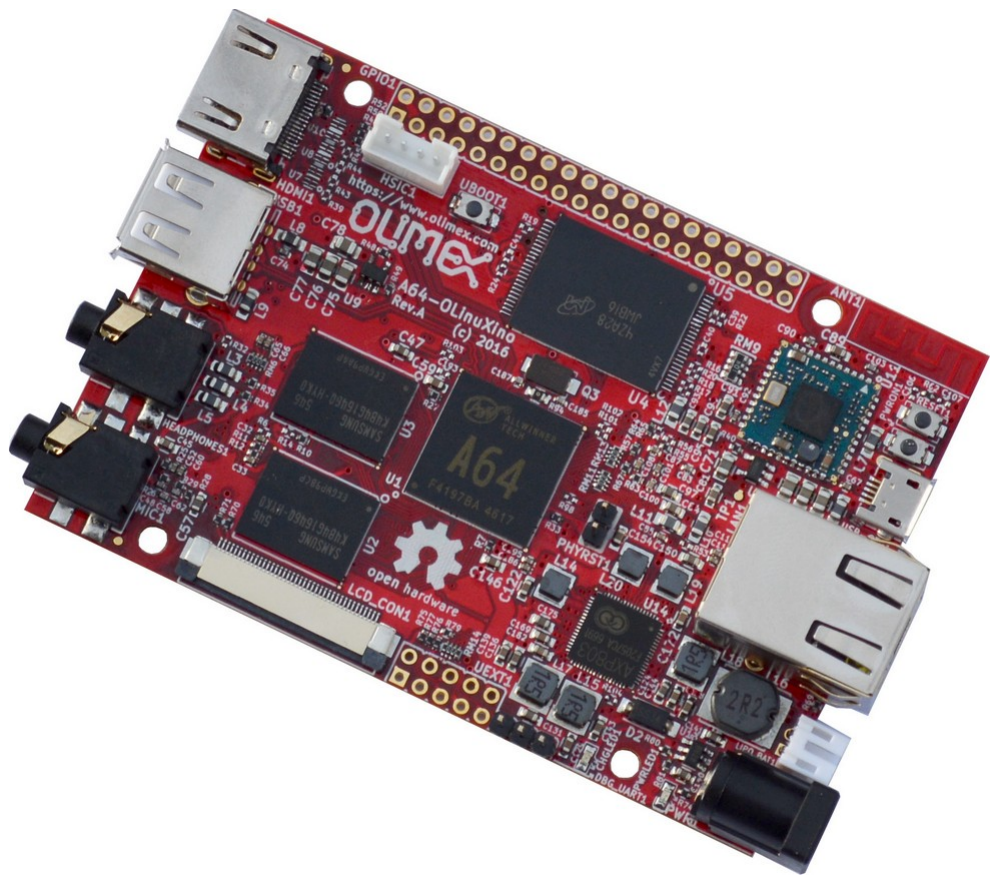
\includegraphics[max width=\linewidth,max height=0.82\textheight]{figuras/figura-31.png}
\label{fig:31}
\caption{Figura 31: A64-OLinuXino é um computador de placa única que roda Linux e Android}
\end{figure}

A64-OLinuXino Olimex A64-OlinuXino é um computador de placa única que roda Linux e Android. O design é baseado em uma CPU ARM de 64 bits e inclui 1 ou 2 GB DDR3 RAM, 4 GB de memória flash, soquete para cartão microSD, WiFi e BLE4.0, Ethernet, HDMI e saída de áudio.

Uma câmera infravermelha de imagem térmica de código aberto CircuitoDigest Com o objetivo de tornar a Câmera Térmica acessível para amadores e fabricantes, construímos esta câmera térmica DIY usando um microcontrolador ESP32 e um sensor térmico MLX90640. A câmera captura

\begin{figure}[H]
\centering
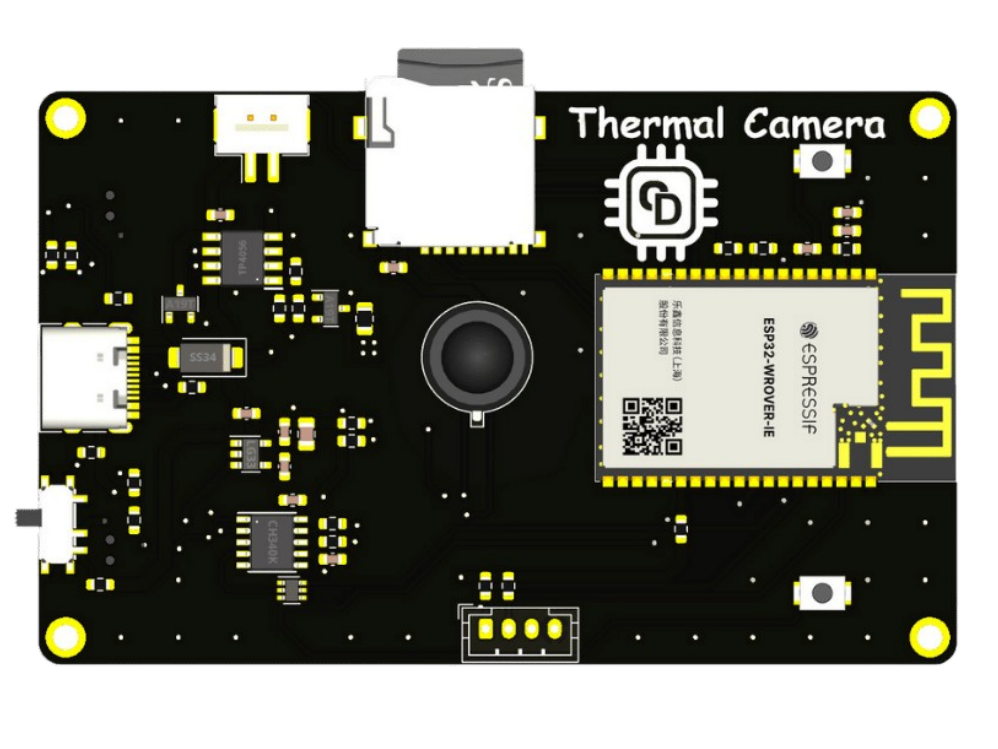
\includegraphics[max width=\linewidth,max height=0.82\textheight]{figuras/figura-32.png}
\label{fig:32}
\caption{Figura 32: Uma câmera infravermelha de imagem térmica de código aberto}
\end{figure}

imagens térmicas com uma resolução de 32x24 pixels e possui uma tela de 2,4 polegadas para visualização. Ela oferece taxas de atualização ajustáveis, várias paletas de cores e recursos de medição de temperatura entre -40°C e 300°C.

\begin{figure}[H]
\centering
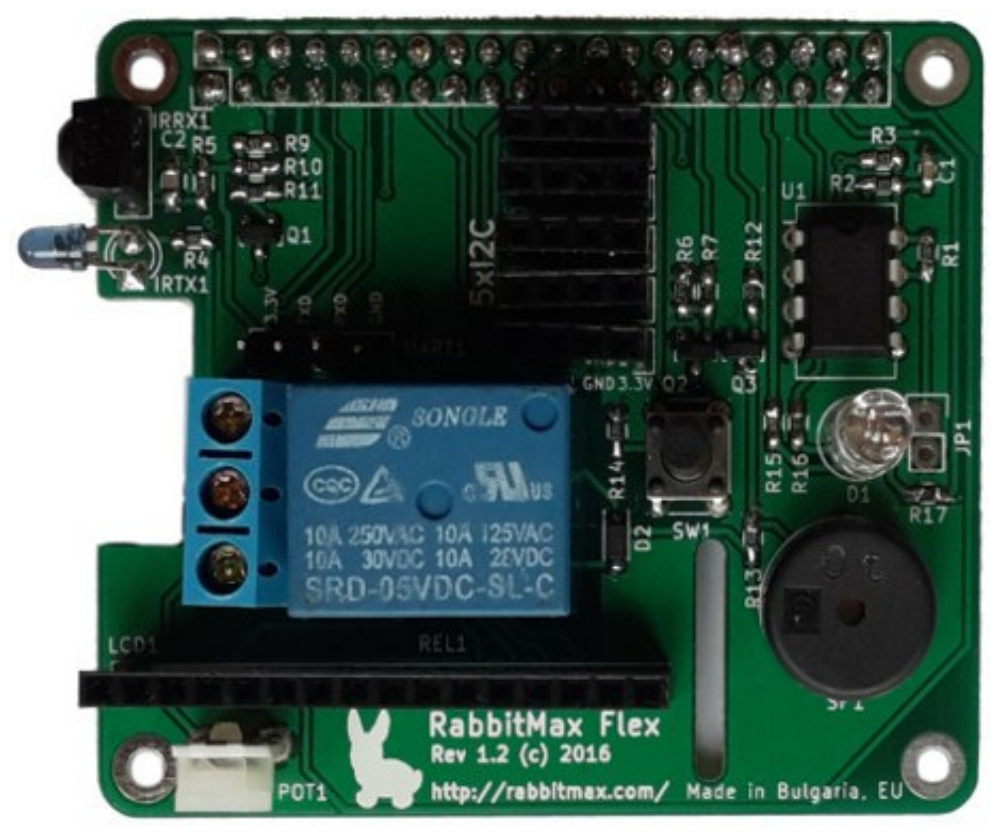
\includegraphics[max width=\linewidth,max height=0.82\textheight]{figuras/figura-33.png}
\label{fig:33}
\caption{Figura 33: ANAVI Flex é um Raspberry Pi Shield de código aberto para prototipagem de IoT e aplicações de automação residencial}
\end{figure}

Shield Flex ANAVI Leon Anavi ANAVI Flex é um Shield Raspberry Pi de código aberto para prototipagem de IoT e aplicações de automação residencial. Ele tem receptor e transmissor infravermelho, relé, campainha, botão, LED RGB e pinos UART para depuração. A placa também suporta módulo de display LCD 1602 e até 5 sensores I2C

\begin{figure}[H]
\centering
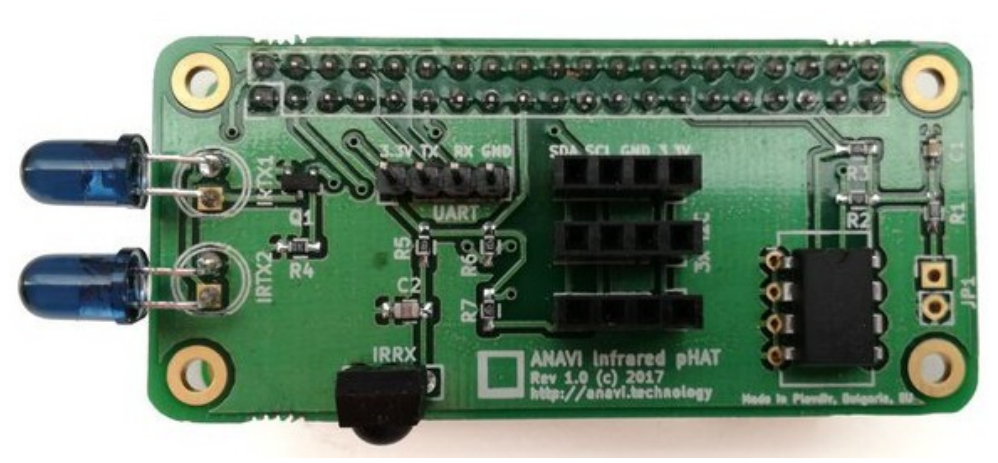
\includegraphics[max width=\linewidth,max height=0.82\textheight]{figuras/figura-34.png}
\label{fig:34}
\caption{Figura 34: ANAVI Infrared pHAT é uma placa adicional que converte o Raspberry Pi em um poderoso controle remoto}
\end{figure}

ANAVI pHAT infravermelho Leon Anavi ANAVI Infrared pHAT é uma placa adicional que converte o Raspberry Pi em um poderoso controle remoto. Ela possui dois transmissores IR, receptor IR, três slots para módulos de sensor I2C, pinos UART para depuração e EEPROM com informações do fabricante da placa.

\begin{figure}[H]
\centering
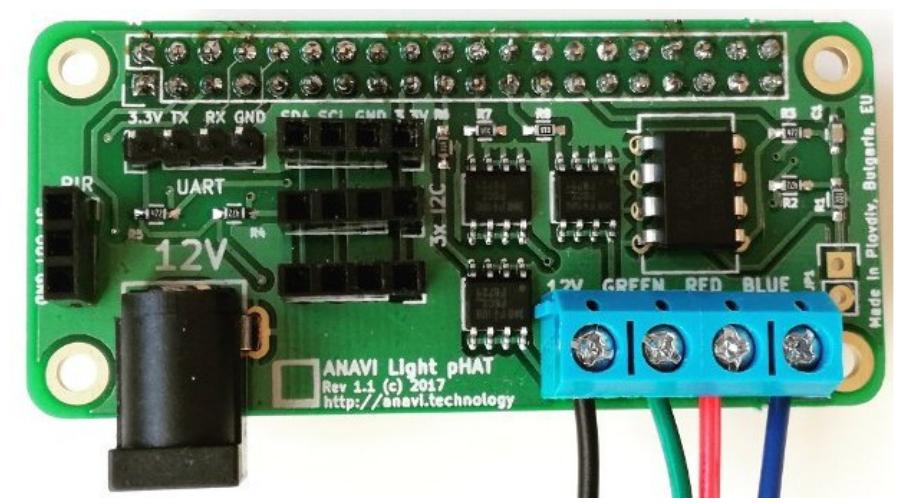
\includegraphics[max width=\linewidth,max height=0.82\textheight]{figuras/figura-35.png}
\label{fig:35}
\caption{Figura 35: ANAVI Light pHAT é uma placa add-on Raspberry Pi para controlar tiras de LED RGB de 12 V}
\end{figure}

ANAVI pHAT leve Leon Anavi ANAVI Light pHAT é uma placa add-on Raspberry Pi para controlar tiras de LED RGB de 12 V. Além disso, tem três slots para módulos de sensor I2C, slot para sensor de movimento PIR, pinos UART para depuração e EEPROM com informações do fabricante da placa.

\begin{figure}[H]
\centering
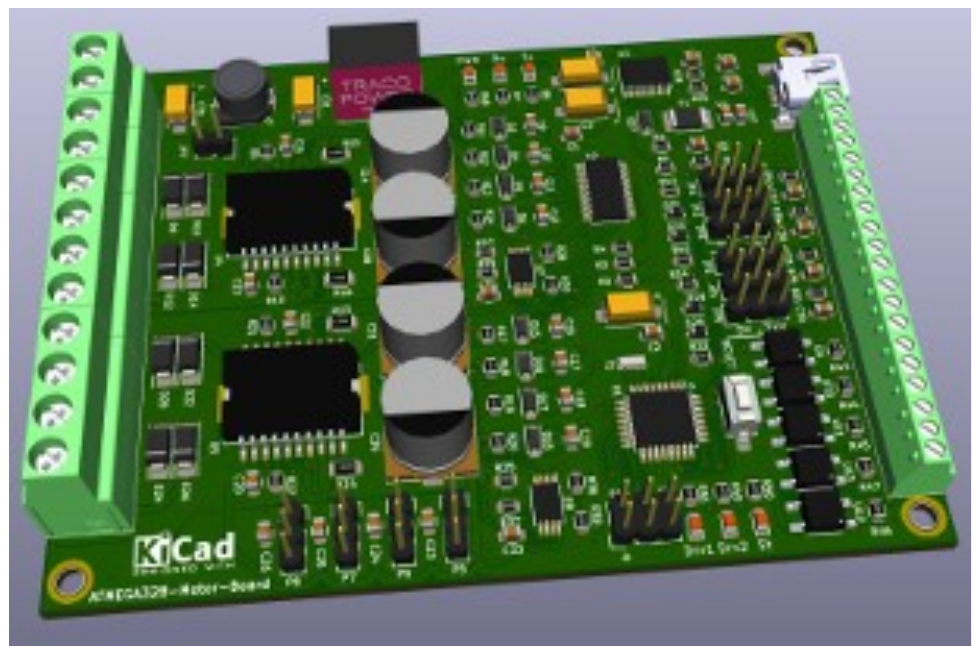
\includegraphics[max width=\linewidth,max height=0.82\textheight]{figuras/figura-36.png}
\label{fig:36}
\caption{Figura 36: controlador de motor de uso geral projetado com kicad em torno do microcontrolador ATmega328 e driver de motor L298P}
\end{figure}

Placa ATMEGA328 para motor Antonio Morales Um controlador de motor de uso geral projetado com kicad em torno do microcontrolador ATmega328 e driver de motor L298P. Ele pode acionar quatro motores com várias opções de entrada.

\begin{figure}[H]
\centering
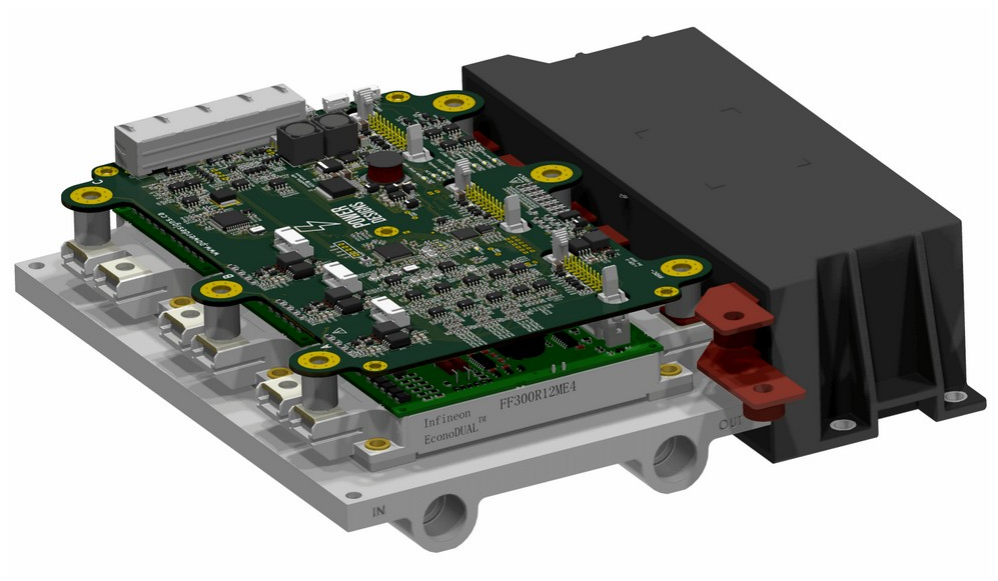
\includegraphics[max width=\linewidth,max height=0.82\textheight]{figuras/figura-37.png}
\label{fig:37}
\caption{Figura 37: Projetos de energia elétrica EV Inc.~Axiom é um controlador de motor de 100kW+ de alta potência e alto desempenho baseado na plataforma VESC}
\end{figure}

Controlador de motor Axiom Projetos de energia elétrica EV Inc.~Axiom é um controlador de motor de 100kW+ de alta potência e alto desempenho baseado na plataforma VESC para compatibilidade com firmware e GUI. Ele é projetado para acionar IGBTs de 650V 600A e vem com muitos recursos de segurança.

\begin{figure}[H]
\centering
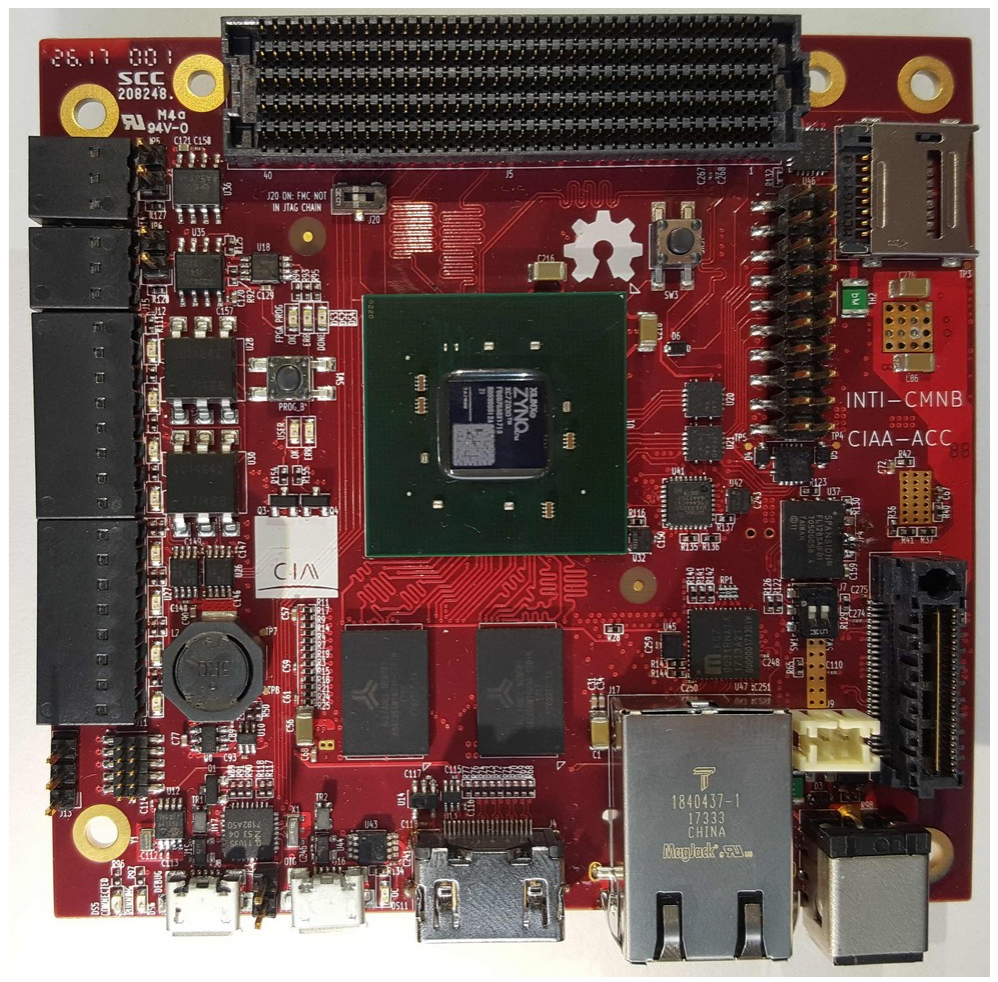
\includegraphics[max width=\linewidth,max height=0.82\textheight]{figuras/figura-38.png}
\label{fig:38}
\caption{Figura 38: O Projeto CIAA é um projeto de hardware e software aberto iniciado para alavancar o ambiente industrial argentino}
\end{figure}

CIAA-ACC (HPC) O Projeto CIAA O Projeto CIAA é um projeto de hardware e software aberto iniciado para alavancar o ambiente industrial argentino. O CIAA-ACC é um projeto de PCB de 12 camadas para Computação de Alto Desempenho. Ele tem um Xilinx Zynq-7000 SoC com uma CPU ARM 2x Cortex A9 e um FPGA Kintex-7. O fator de forma é o PCIe-104 expansível. Periféricos: memória DDR3 de 1 GB, Quad SPI Flash, Gbit Ethernet, Micro SDHC, USB 2.0, HDMI de dupla função, PCIe 1x

\begin{figure}[H]
\centering
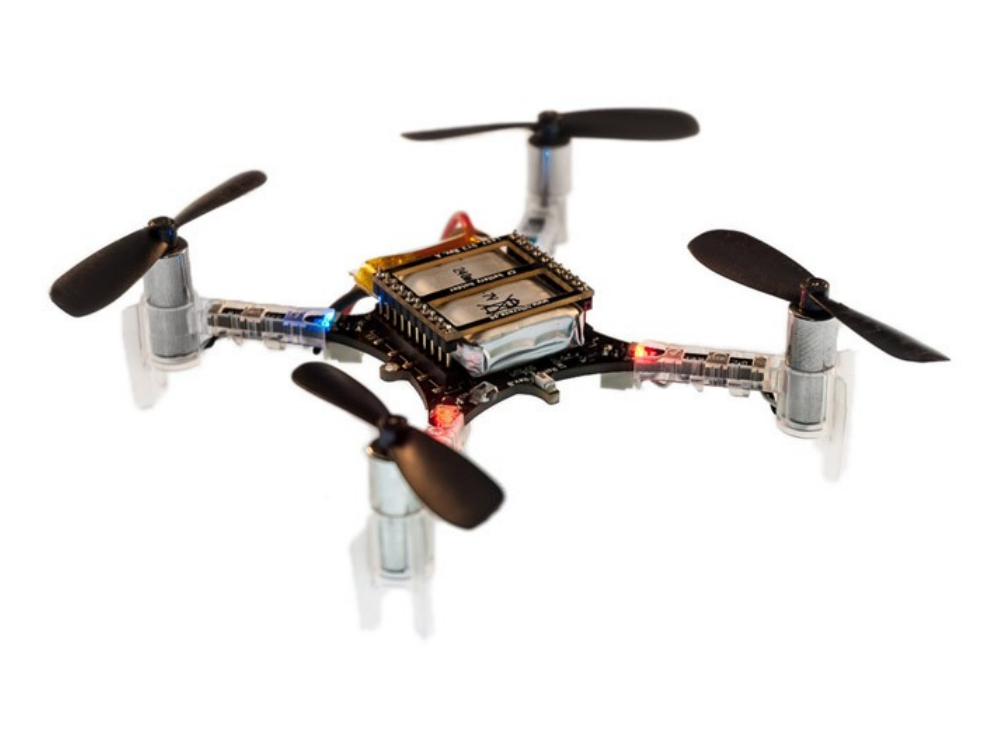
\includegraphics[max width=\linewidth,max height=0.82\textheight]{figuras/figura-39.png}
\label{fig:39}
\caption{Figura 39: O Crazyflie 1.0 é uma plataforma de desenvolvimento de voo aberto}
\end{figure}

Crazyflie 1.0 Bitcraze AB O Crazyflie 1.0 é uma plataforma de desenvolvimento de voo aberto. É uma plataforma versátil que inclui um poderoso MCU Cortex-M4, rádio de baixa latência de 2,4 GHz e bluetooth de baixa energia. Ele também tem uma porta de expansão que permite adicionar facilmente hardware extra.

\begin{figure}[H]
\centering
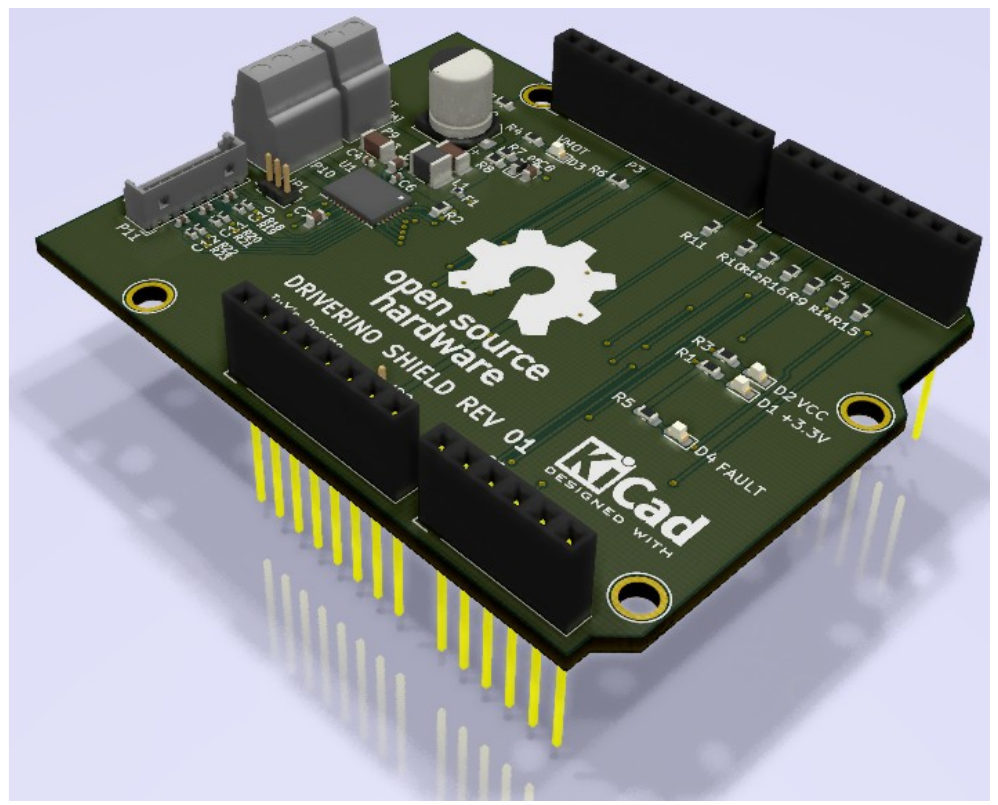
\includegraphics[max width=\linewidth,max height=0.82\textheight]{figuras/figura-40.png}
\label{fig:40}
\caption{Figura 40: Driverino-Shield é um controlador simples e de baixo consumo para motores BLDC sensorizados}
\end{figure}

Shield Driverino Michele Santucci Driverino-Shield é um controlador simples e de baixo consumo para motores BLDC sensorizados. O objetivo do projeto era criar um shield Arduino capaz de acionar um motor PM BLDC com potência de cerca de 50-100 W. A placa é equipada com driver TI MCT8316Z BLDC.

\begin{figure}[H]
\centering
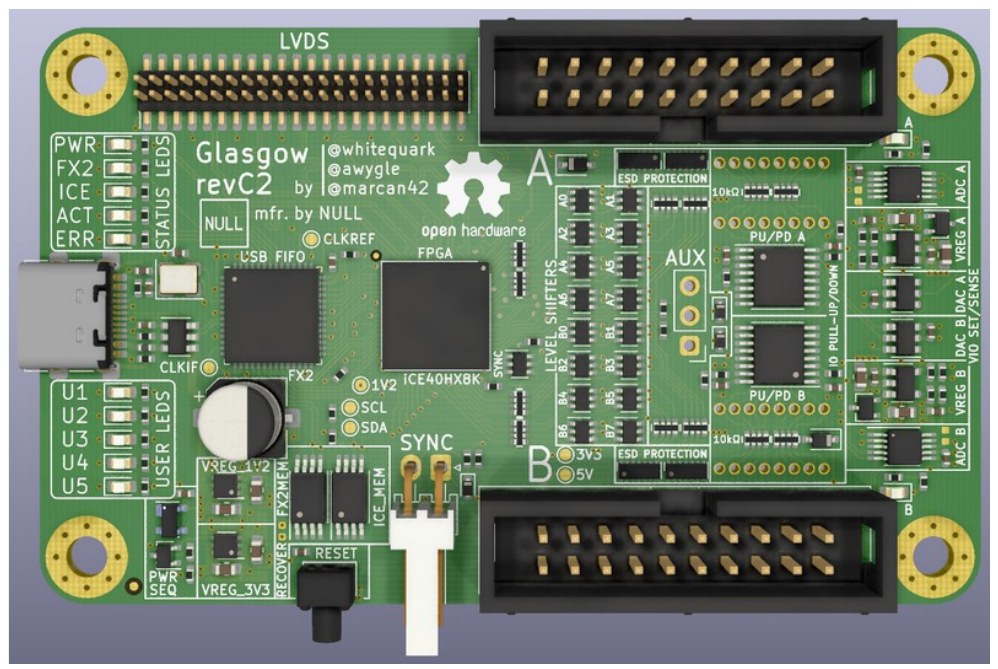
\includegraphics[max width=\linewidth,max height=0.82\textheight]{figuras/figura-41.png}
\label{fig:41}
\caption{Figura 41: Glasgow é uma ferramenta para explorar interfaces digitais, destinada a desenvolvedores embarcados, engenharia reversa e outras utilidades}
\end{figure}

RevC de Glasgow Catarina `quark branco' Glasgow é uma ferramenta para explorar interfaces digitais, destinada a desenvolvedores embarcados, engenharia reversa, arquivamento digitais, entusiastas de eletrônica e todos os outros que desejam se comunicar com uma ampla seleção de dispositivos digitais com alta confiabilidade e o mínimo de complicações.

\begin{figure}[H]
\centering
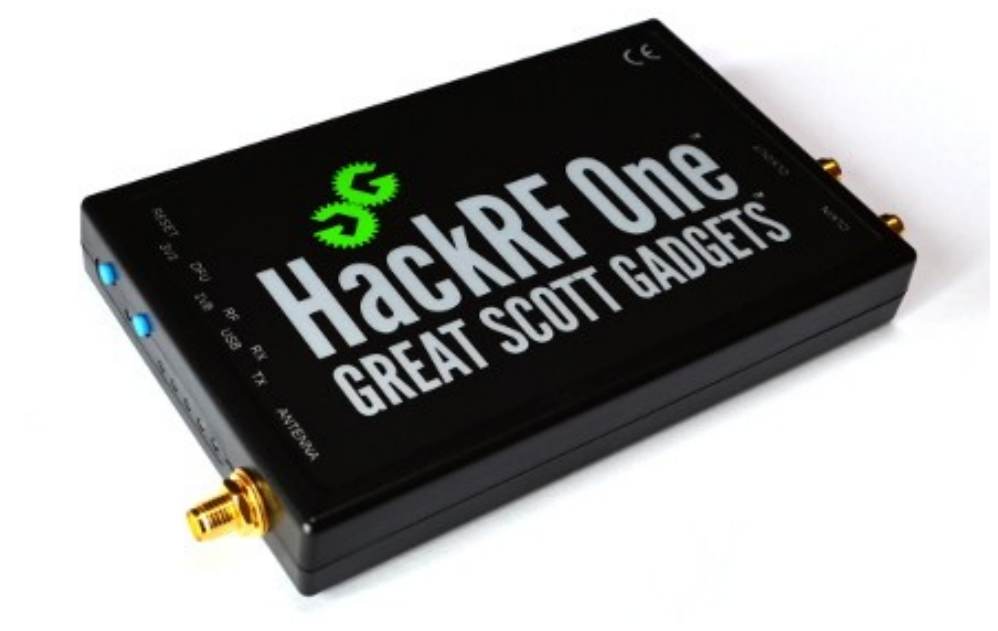
\includegraphics[max width=\linewidth,max height=0.82\textheight]{figuras/figura-42.png}
\label{fig:42}
\caption{Figura 42: HackRF One da Great Scott Gadgets é um periférico de Rádio Definido por Software capaz de transmitir ou receber sinais de rádio de 1 MHz a 6 GHz}
\end{figure}

HackRF Grandes Gadgets Scott HackRF One da Great Scott Gadgets é um periférico de Rádio Definido por Software capaz de transmitir ou receber sinais de rádio de 1 MHz a 6 GHz. Projetado para permitir testes e desenvolvimento de tecnologias de rádio modernas e de próxima geração, HackRF One é uma plataforma de hardware de código aberto que pode ser usada como um periférico USB ou programada para operação autônoma.

\begin{figure}[H]
\centering
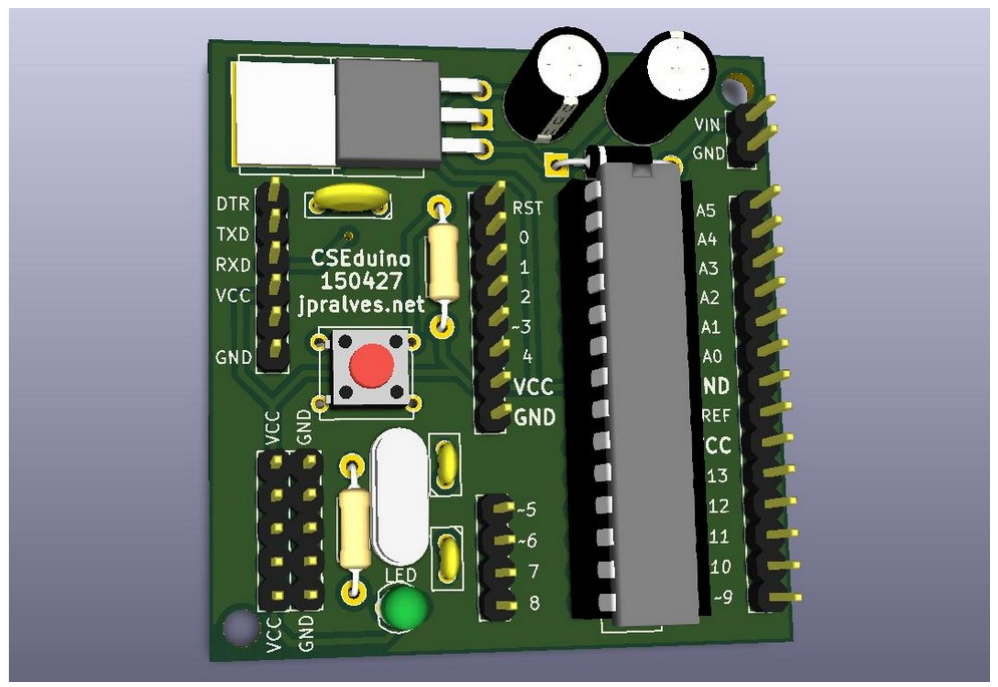
\includegraphics[max width=\linewidth,max height=0.82\textheight]{figuras/figura-43.png}
\label{fig:43}
\caption{Figura 43: CSEduino é a resposta para uma placa DIY Arduino de custo muito baixo}
\end{figure}

CSEduino v4 João Alves CSEduino é a resposta para uma placa DIY Arduino de custo muito baixo. Esta versão tem um pcb de 2 camadas criado com kicad.

\begin{figure}[H]
\centering
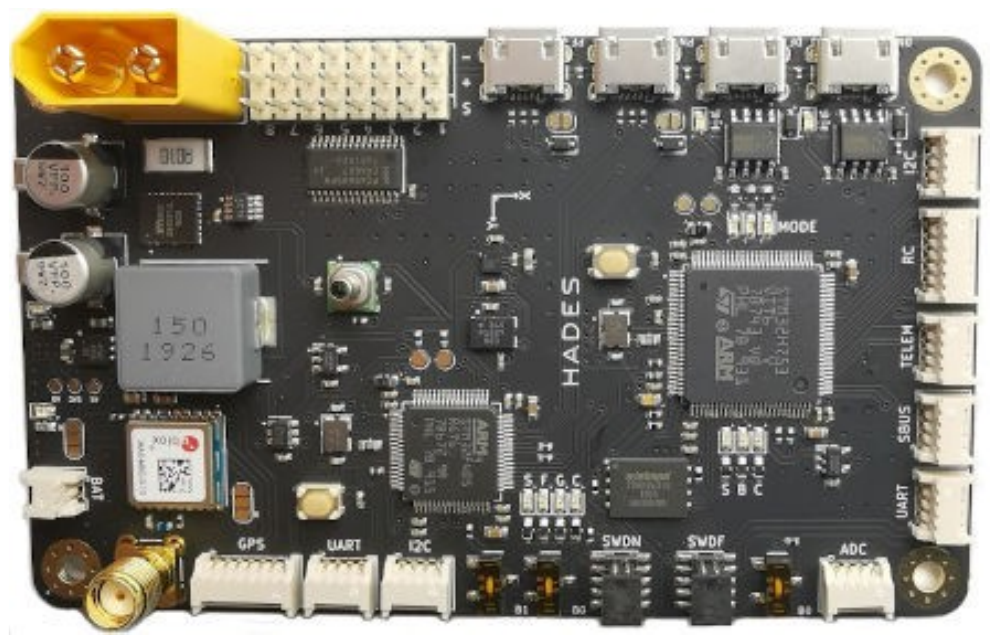
\includegraphics[max width=\linewidth,max height=0.82\textheight]{figuras/figura-44.png}
\label{fig:44}
\caption{Figura 44: HADES FCS é um sistema de controle de voo de código aberto para veículos aéreos não tripulados (UAVs) projetado completamente do zero}
\end{figure}

Sistema de controle de voo HADES Filipe Salmony HADES FCS é um sistema de controle de voo de código aberto para veículos aéreos não tripulados (UAVs) projetado completamente do zero. Isso inclui o hardware (PCBs de controle de voo personalizados), firmware STM32 (usando FreeRTOS), filtragem de Kalman para estimativa de estado, algoritmos de controle, estação base, protocolo de comunicação, simulador de voo, processamento de sinal e muito, muito mais.

\begin{figure}[H]
\centering
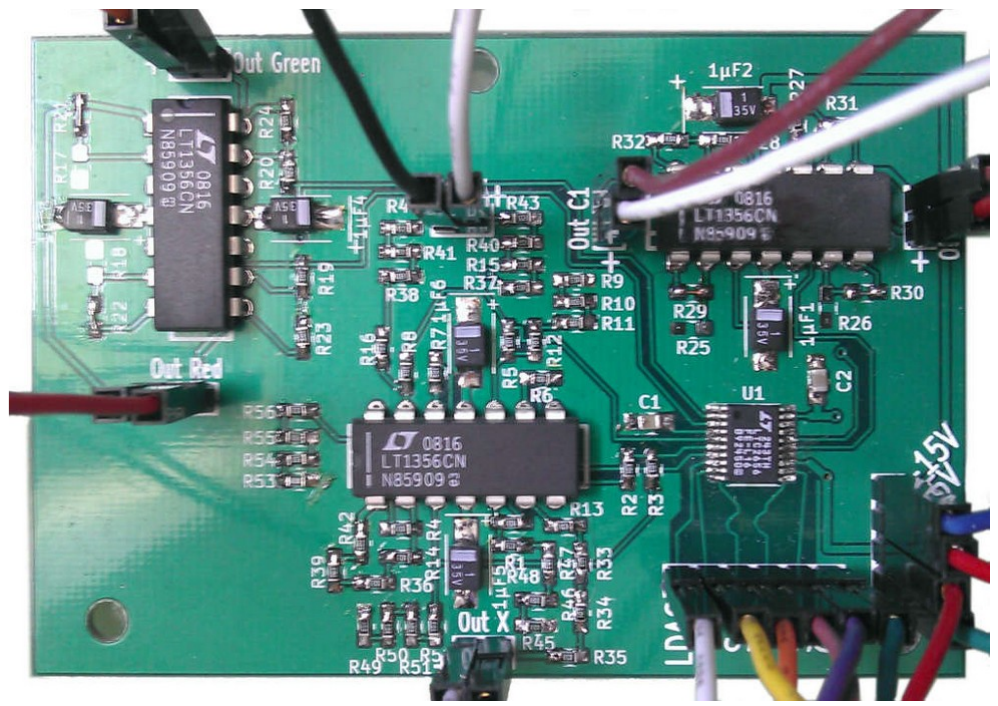
\includegraphics[max width=\linewidth,max height=0.82\textheight]{figuras/figura-45.png}
\label{fig:45}
\caption{Figura 45: O JEMTech-ILDA-Node é um DAC de 16 bits e 6 canais para ILDA de até 400 kpps}
\end{figure}

JEMTech-ILDA-Node Jan-Erik Matthies O JEMTech-ILDA-Node é um DAC de 16 bits e 6 canais para ILDA de até 400 kpps. Este Projeto é um DAC (conversor digital para analógico) que gera seis sinais diferenciais com base no padrão ILDA (International Laser Display Association) ISP-DB25. O DAC é controlado via barramento SPI (Serial Peripheral Interface).

\begin{figure}[H]
\centering
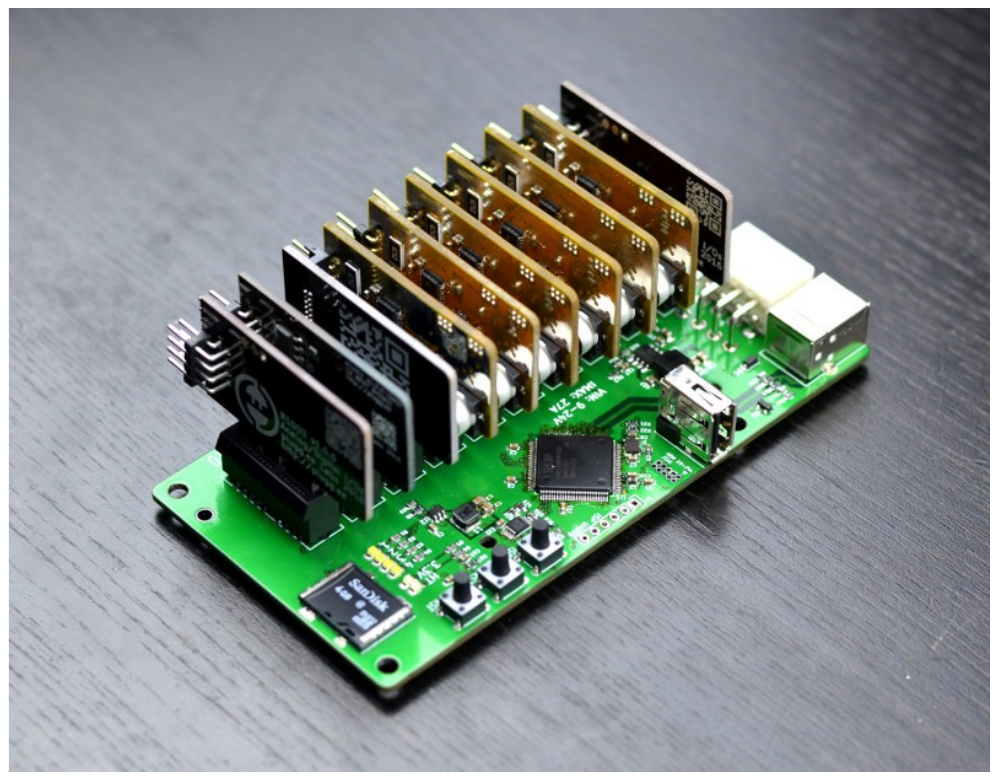
\includegraphics[max width=\linewidth,max height=0.82\textheight]{figuras/figura-46.png}
\label{fig:46}
\caption{Figura 46: Quadro Suculento-JuicyBoard do plugg.ee Labs é uma plataforma de robótica modular de código aberto que pode ser usada para construir impressoras 3D personalizadas, máquinas CNC e muito mais}
\end{figure}

Quadro Suculento Laboratórios plugg.ee JuicyBoard do plugg.ee Labs é uma plataforma de robótica modular de código aberto que pode ser usada para construir impressoras 3D personalizadas, máquinas CNC e muito mais.

\begin{figure}[H]
\centering
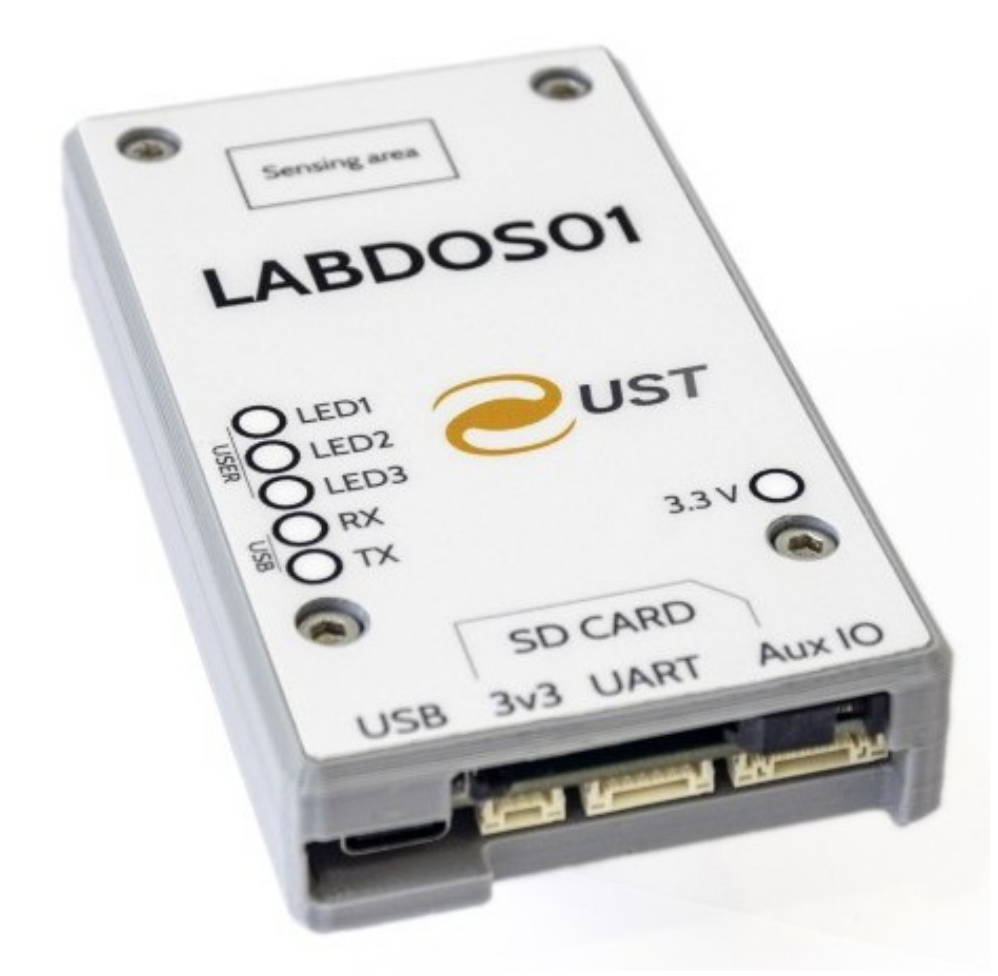
\includegraphics[max width=\linewidth,max height=0.82\textheight]{figuras/figura-47.png}
\label{fig:47}
\caption{Figura 47: LABDOS-espectrômetro de radiação ionizante}
\end{figure}

LABDOS-espectrômetro de radiação ionizante baseado em semicondutores Tecnologias Científicas Universais sro (UST) LABDOS01 é um espectrômetro-dosímetro de código aberto baseado em um diodo PIN de silício e é destinado a pesquisas científicas e propósitos experimentais. Uma porta USB-C ou conector JST-GH protege a energia e a comunicação. O dispositivo pode ser usado estaticamente (localizado em um local específico, por exemplo, laboratório ou base) ou em aplicações móveis (como carros ou UAVs). O espectrômetro é alojado em uma caixa impressa em 3D, que traz resistência mecânica essencial e permite o desenvolvimento futuro de gabinetes de usuário e novas integrações. O objetivo do LABDOS01 é criar um dispositivo de medição de código aberto, acessível, de alta qualidade, confiável e simples --- um espectrômetro de energia de radiação para a comunidade científica.

\begin{figure}[H]
\centering
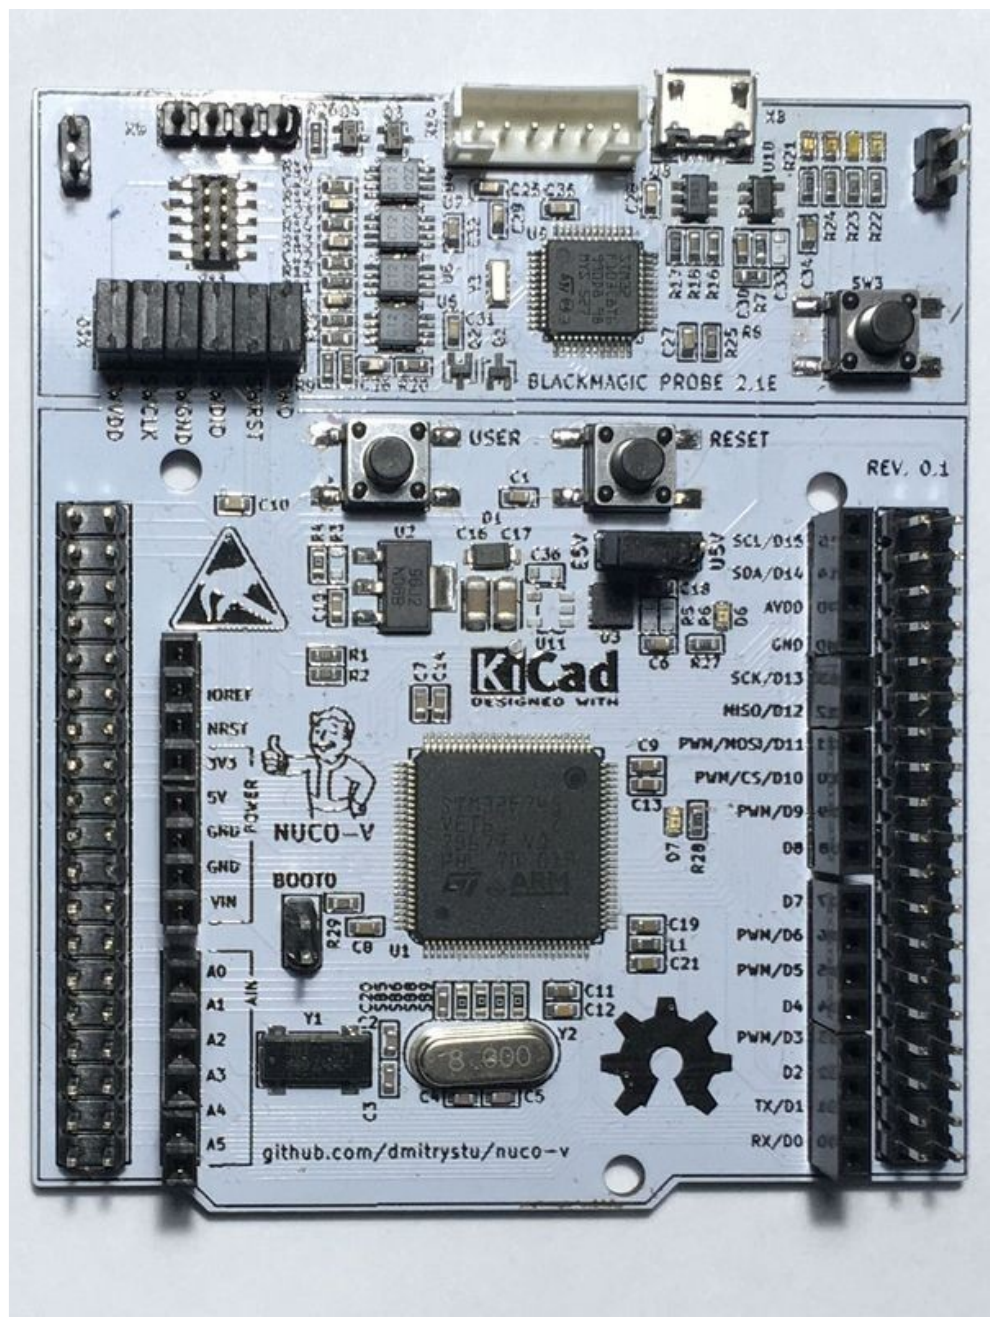
\includegraphics[max width=\linewidth,max height=0.82\textheight]{figuras/figura-48.png}
\label{fig:48}
\caption{Figura 48: NUCO-V-placa de desenvolvimento compatível com NUCLEO-64© para as séries STM32F7 e STM32H7 com Black Magic Probe integrado}
\end{figure}

NUCO-V Dmitry Filimonchuk NUCO-V é uma placa de desenvolvimento compatível com NUCLEO-64© para as séries STM32F7 e STM32H7 com Black Magic Probe integrado

\begin{figure}[H]
\centering
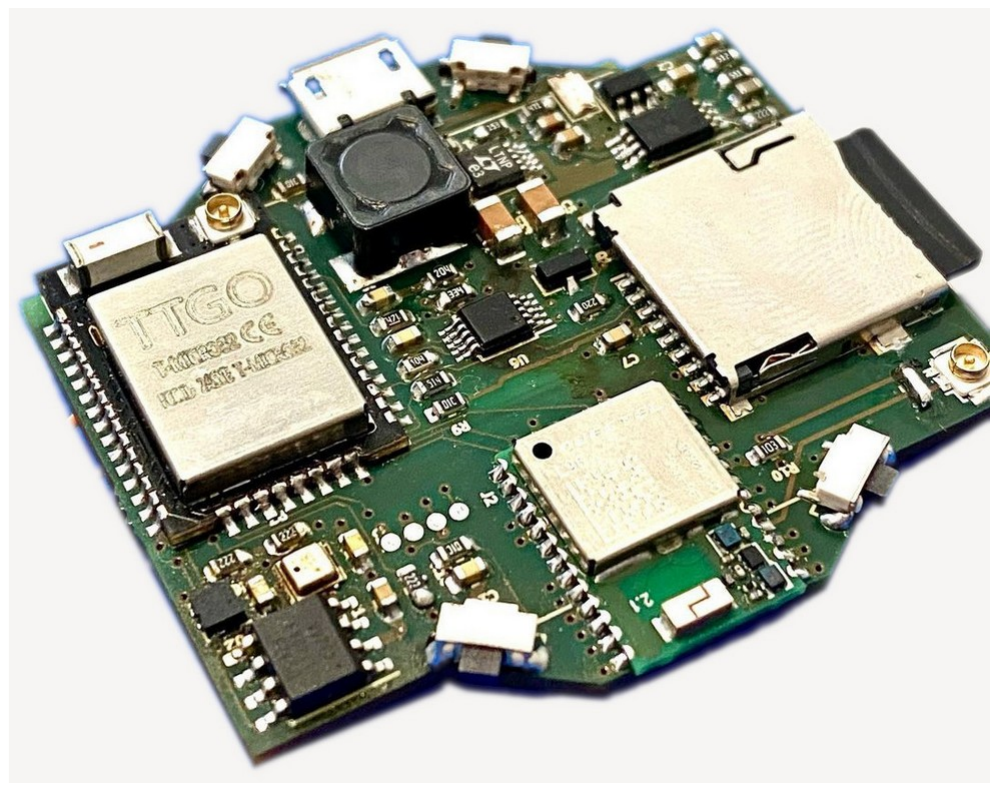
\includegraphics[max width=\linewidth,max height=0.82\textheight]{figuras/figura-49.png}
\label{fig:49}
\caption{Figura 49: Open Smartwatch é um relógio inteligente completamente aberto (ECAD/MCAD e software)}
\end{figure}

Smartwatch aberto pauls\_coisas\_3d Open Smartwatch é um relógio inteligente completamente aberto (ECAD/MCAD e software). O objetivo é construir um smartwatch de código aberto, com rastreamento por GPS e mapas. Os recursos incluem: ESP32, GPS, Time, sensores MEMS, bateria de íons de lítio, USB serial e armazenamento em cartão microSD.

\begin{figure}[H]
\centering
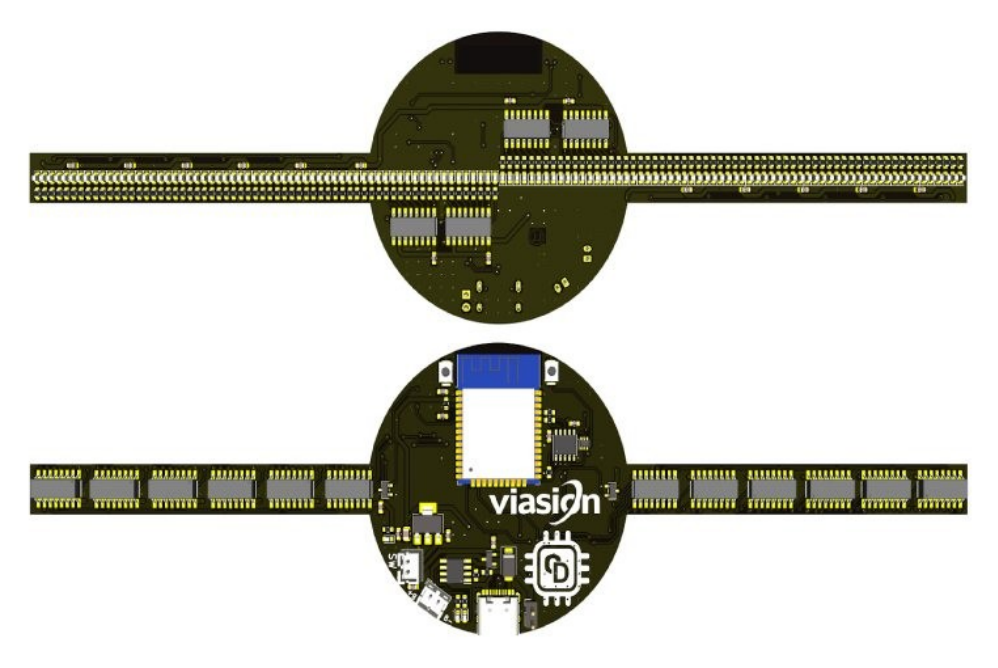
\includegraphics[max width=\linewidth,max height=0.82\textheight]{figuras/figura-50.png}
\label{fig:50}
\caption{Figura 50: display POV de código aberto com resolução de 128 pixels e uma taxa de quadros máxima de 20 FPS}
\end{figure}

Exibição POV de código aberto usando ESP32 Jóbito José Um display POV de código aberto com resolução de 128 pixels e uma taxa de quadros máxima de 20 FPS. Este display é capaz de exibir imagens e animações. O display é construído em torno do ESP32 SoC e usa registradores de deslocamento 74HC595 para controlar cada pixel. Também criamos uma ferramenta da web, que converterá cada imagem em uma matriz que precisa de apenas aproximadamente 2 KB de espaço de código para cada imagem. Isso faz com que seja possível integrar facilmente vários números de imagens no código sem se preocupar com a limitação de armazenamento.

\begin{figure}[H]
\centering
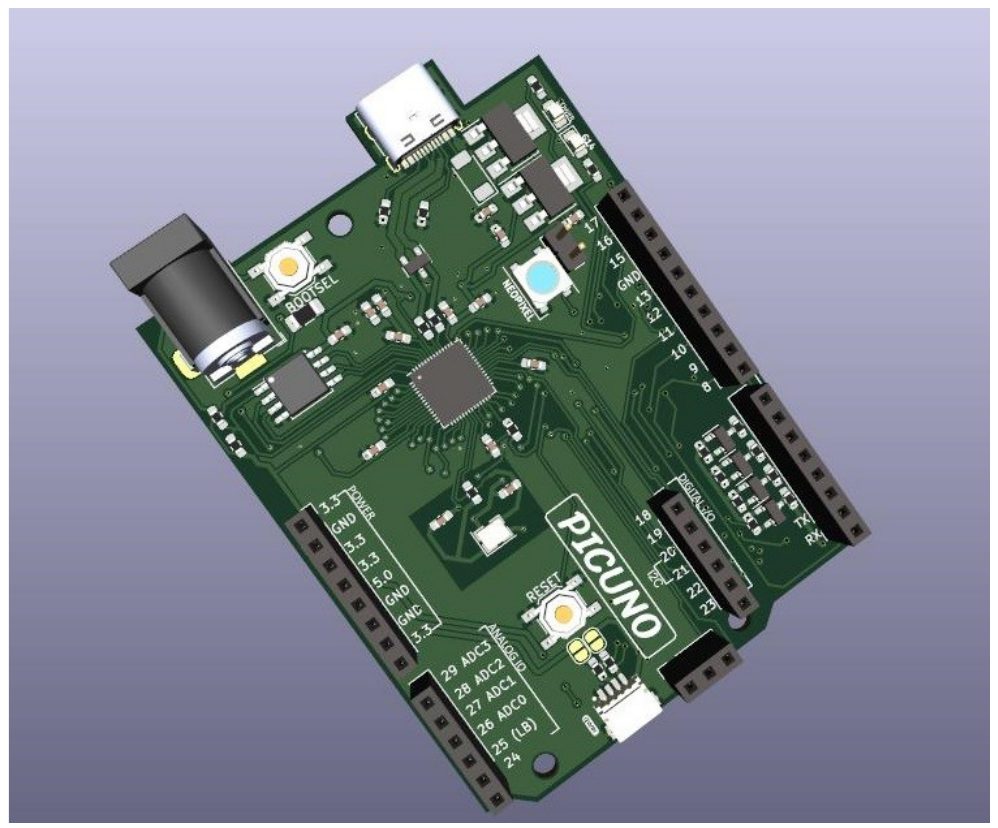
\includegraphics[max width=\linewidth,max height=0.82\textheight]{figuras/figura-51.png}
\label{fig:51}
\caption{Figura 51: O Picuno é a mistura do RP2040 e do Arduino UNO}
\end{figure}

Picuno Atul Ravi O Picuno é a mistura do RP2040 e do Arduino UNO. Um substituto para o UNO compatível com derivados C e python.

\begin{figure}[H]
\centering
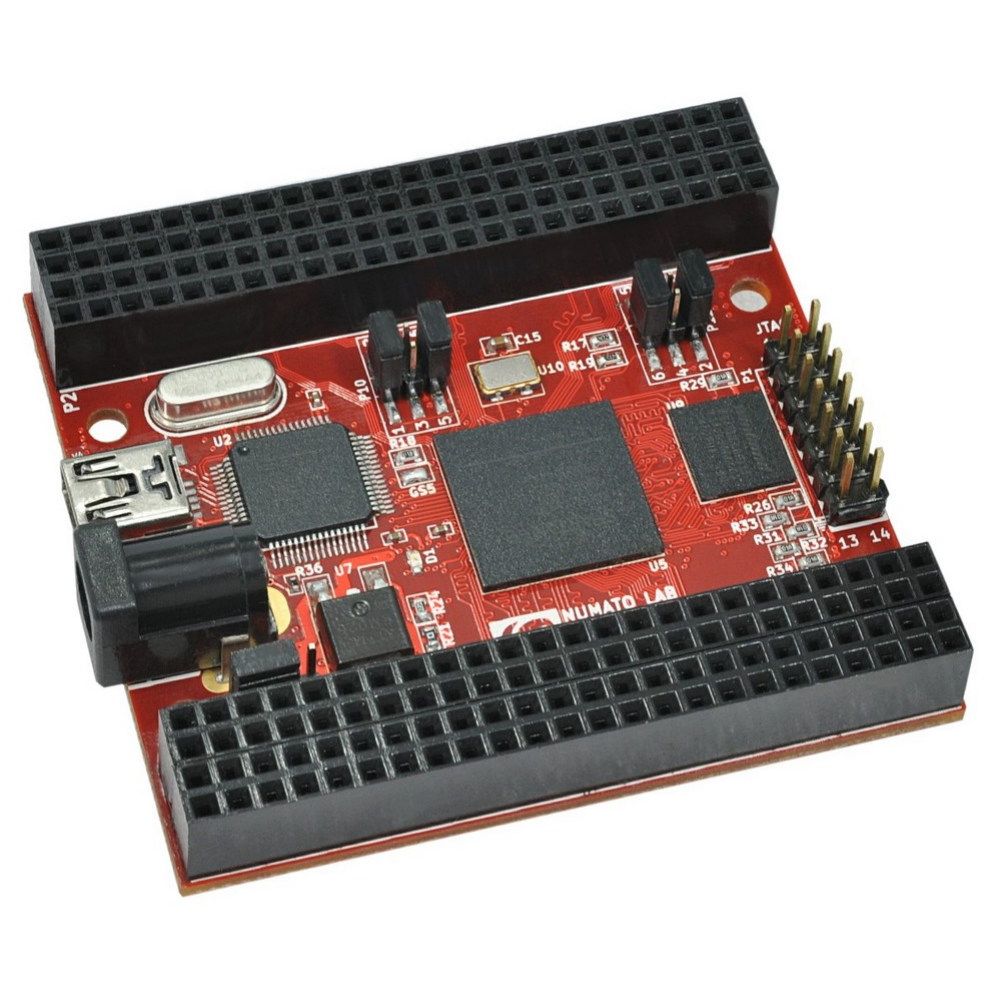
\includegraphics[max width=\linewidth,max height=0.82\textheight]{figuras/figura-52.png}
\label{fig:52}
\caption{Figura 52: Saturn é uma placa de desenvolvimento FPGA fácil de usar com Xilinx Spartan-6 FPGA}
\end{figure}

Saturno Numato Saturn é uma placa de desenvolvimento FPGA fácil de usar com Xilinx Spartan-6 FPGA. Saturn é especialmente projetada para experimentar e aprender design de sistemas com FPGAs. Esta placa de desenvolvimento apresenta FPGA da série Xilinx XC6SLX com dispositivo USB de canal duplo FT2232H da FTDI. A interface USB 2.0 de alta velocidade fornece download de configuração rápido e fácil para o flash SPI integrado. Nenhum programador ou cabo de downloader especial é necessário para baixar o fluxo de bits para a placa.

\begin{figure}[H]
\centering
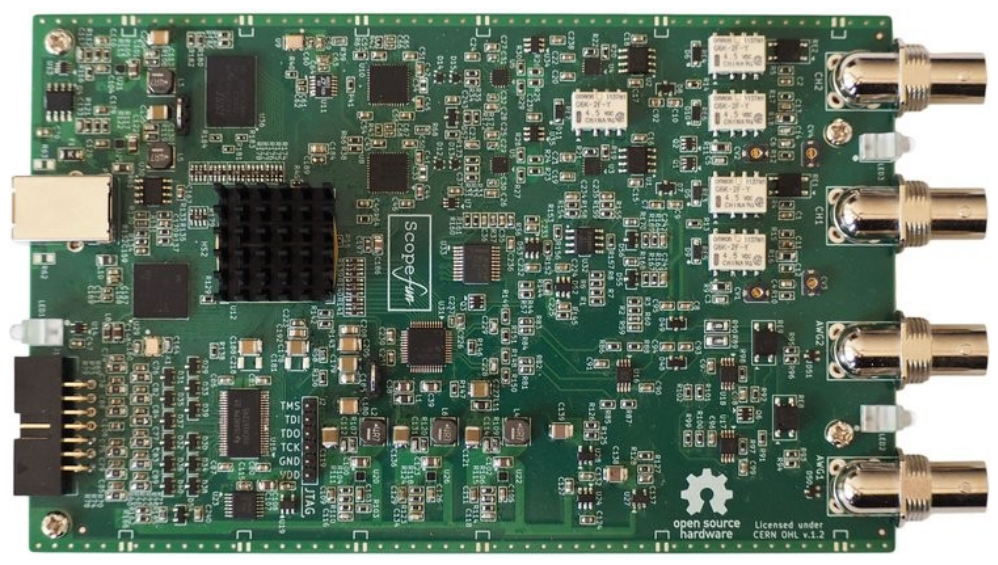
\includegraphics[max width=\linewidth,max height=0.82\textheight]{figuras/figura-53.png}
\label{fig:53}
\caption{Figura 53: ScopeFun é uma plataforma de instrumentação tudo-em-um de código aberto}
\end{figure}

ScopeFun Dejan Priversek e David Kosenina ScopeFun é uma plataforma de instrumentação tudo-em-um de código aberto. Inclui um osciloscópio, gerador de forma de onda arbitrária, analisador de espectro, analisador lógico e gerador de padrão digital.

\begin{figure}[H]
\centering
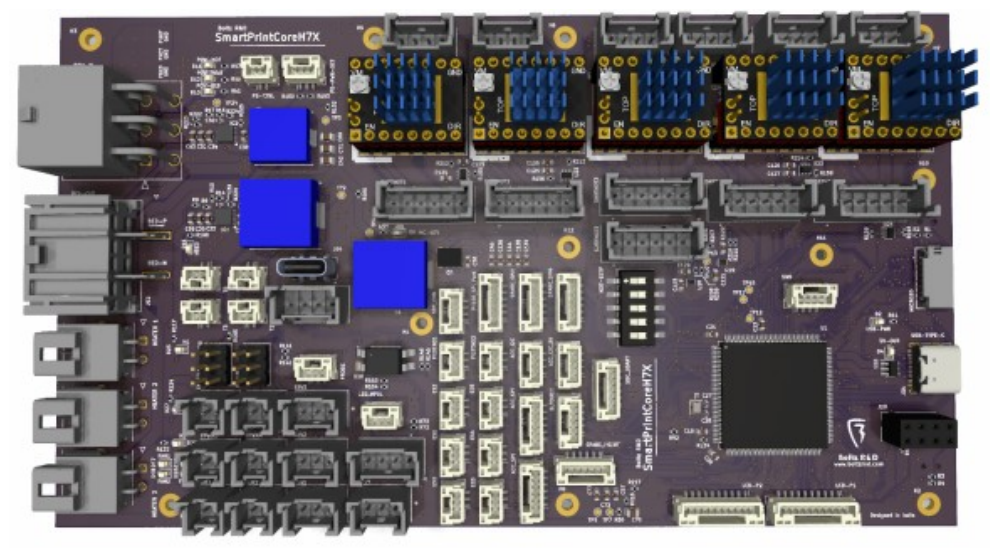
\includegraphics[max width=\linewidth,max height=0.82\textheight]{figuras/figura-54.png}
\label{fig:54}
\caption{Figura 54: SmartPrintCoreH7x-controladora 3D}
\end{figure}

SmartPrintCoreH7x Boltz P\&D Mergulhe no coração da inovação com o SmartPrintCoreH7x, uma inovadora placa-mãe de impressora 3D de código aberto projetada com paixão pela comunidade e um foco claro em durabilidade, confiabilidade e facilidade de uso. Nascida de uma visão para capacitar fabricantes, inventores e engenheiros ao redor do mundo, a SmartPrintCoreH7x se prepara para se tornar um farol de desenvolvimento colaborativo no mundo da impressão 3D

\hypertarget{dosuxedmetros-spacedos}{%
\subsubsection{Dosímetros SPACEDOS}\label{dosuxedmetros-spacedos}}

Tecnologias Científicas Universais sro (UST)

Os dosímetros SPACEDOS são espectrômetros e dosímetros de radiação ionizante baseados em detectores semicondutores de código aberto. Eles já

\begin{figure}[H]
\centering
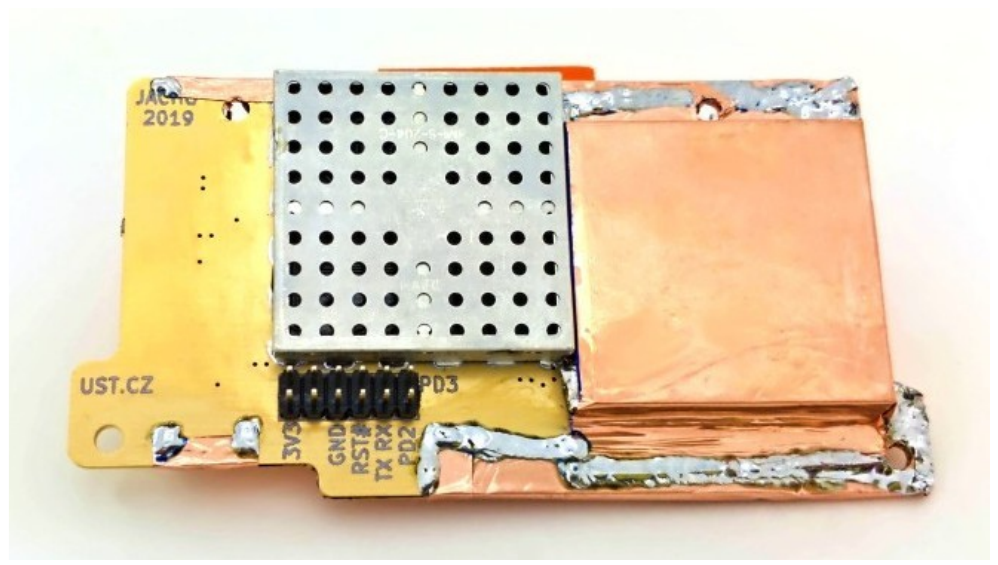
\includegraphics[max width=\linewidth,max height=0.82\textheight]{figuras/figura-55.png}
\label{fig:55}
\caption{Figura 55: dosímetros SPACEDOS são espectrômetros e dosímetros de radiação ionizante baseados em detectores semicondutores de código aberto}
\end{figure}

participaram com sucesso de várias

\emph{espectrômetros e dosímetros de radiação}

missões espaciais. O SPACEDOS02 mede,

\emph{ionizante baseados em detectores}

\emph{semicondutores de código aberto.}

por um período de troca regular de tripulação com duração de vários meses, a bordo da Estação Espacial Internacional (ISS). O dosímetro SPACEDOS01 foi modificado para montagem dentro de CubeSats e foi enviado para a órbita da Terra como parte do satélite SOCRAT-R.

\begin{figure}[H]
\centering
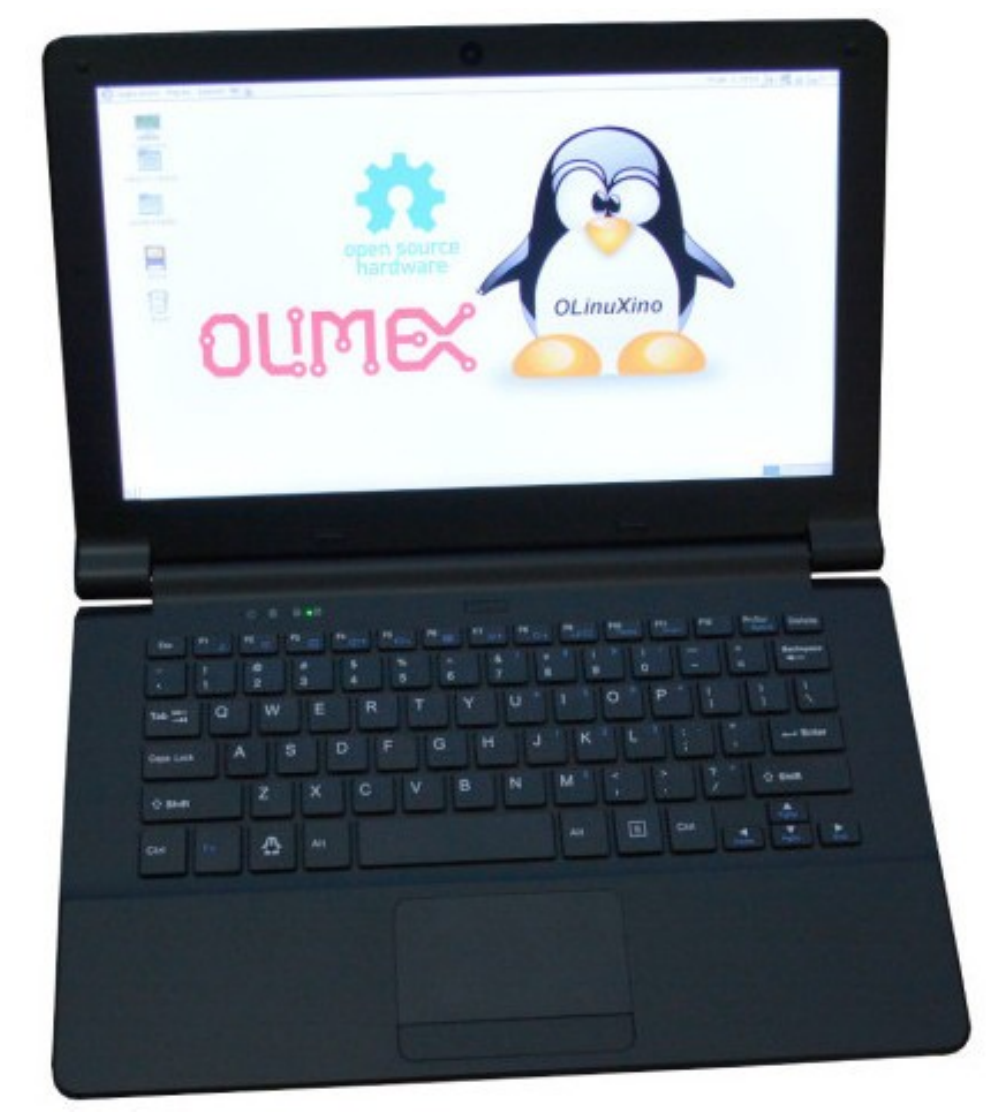
\includegraphics[max width=\linewidth,max height=0.82\textheight]{figuras/figura-56.png}
\label{fig:56}
\caption{Figura 56: O TERES I é um laptop de hardware e software de código aberto}
\end{figure}

Teres I Olimex O TERES I é um laptop de hardware e software de código aberto do tipo ``faça você mesmo'' com processadores ARM64 e x86, incluindo arquivos MCAD.

\begin{figure}[H]
\centering
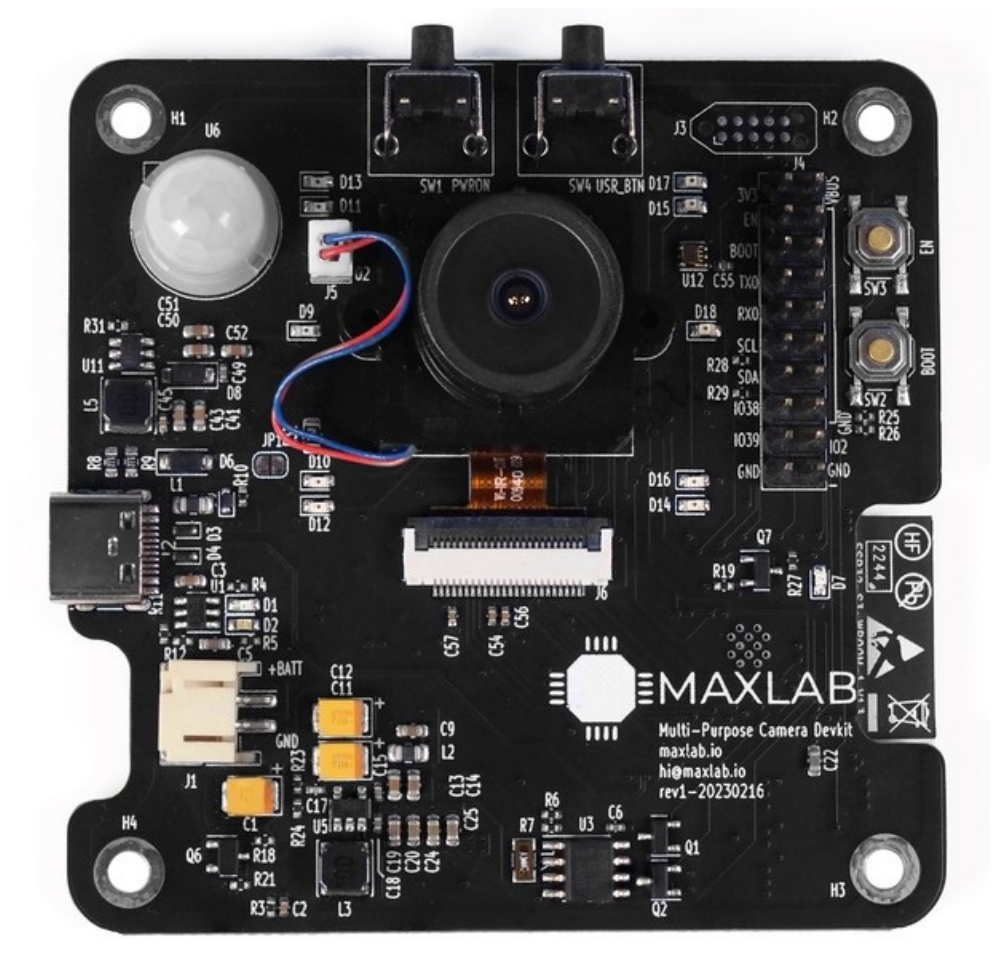
\includegraphics[max width=\linewidth,max height=0.82\textheight]{figuras/figura-57.png}
\label{fig:57}
\caption{Figura 57: Tokay Lite: Câmera ESP32 Edge AIMAXLAB.IO}
\end{figure}

Tokay Lite: Câmera ESP32 Edge AI MAXLAB.IO Tokay Lite é a placa de desenvolvimento de câmera ESP32 ideal para aplicações de processamento de imagem de baixo consumo de energia na borda. O Tokay Lite pode ser usado como um devkit independente para auxiliar desenvolvedores com uma ferramenta conveniente ou ser incorporado a um sistema maior para aumentá-lo com dados de visão e processamento de imagem.

\begin{figure}[H]
\centering
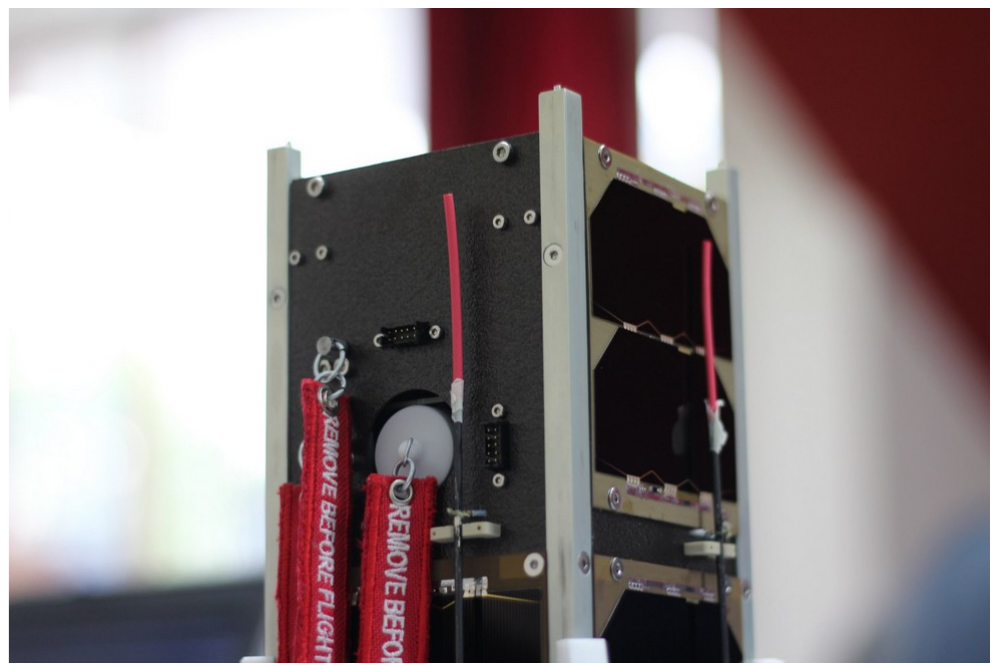
\includegraphics[max width=\linewidth,max height=0.82\textheight]{figuras/figura-58.png}
\label{fig:58}
\caption{Figura 58: O primeiro satélite da UPSat Cubesat 2U construído e entregue pela Libre Space}
\end{figure}

UPSat Fundação Espaço Livre O primeiro satélite de código aberto O UPSat é um satélite Cubesat 2U construído e entregue pela Libre Space Foundation, iniciado pela Universidade de Patras como parte da missão upsatQB50 com ID GR-02.

\begin{figure}[H]
\centering
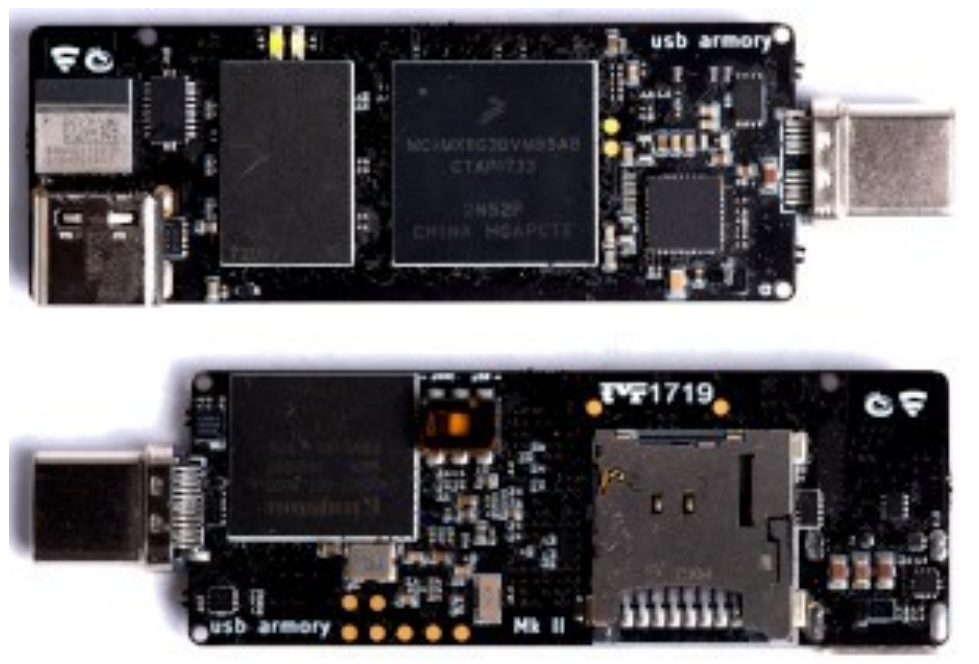
\includegraphics[max width=\linewidth,max height=0.82\textheight]{figuras/figura-59.png}
\label{fig:59}
\caption{Figura 59: O arsenal USB 2 da Inverse Path é um projeto de hardware de código aberto que implementa um computador do tamanho de um pen drive}
\end{figure}

Armaria USB Mk II Caminho inverso / F-Secure O arsenal USB da Inverse Path é um projeto de hardware de código aberto que implementa um computador do tamanho de um pen drive. O dispositivo compacto alimentado por USB fornece uma plataforma para desenvolver e executar uma variedade de aplicativos.

\hypertarget{controle-de-impeduxe2ncia-em-circuitos-de-alta-frequuxeancia}{%
\chapter{Controle de impedância em circuitos de alta frequência}\label{controle-de-impeduxe2ncia-em-circuitos-de-alta-frequuxeancia}}

O \textbf{controle de impedância} no design de PCBs é essencial em projetos que envolvem sinais de alta frequência ou transmissão de dados em alta velocidade. Ele garante que as características elétricas das trilhas estejam adequadas para preservar a integridade do sinal, minimizar perdas e evitar reflexões ou interferências.

\hypertarget{importuxe2ncia-do-controle-de-impeduxe2ncia}{%
\section{Importância do controle de impedância}\label{importuxe2ncia-do-controle-de-impeduxe2ncia}}

\begin{enumerate}
\def\labelenumi{\arabic{enumi}.}
\item
  \textbf{Integridade do Sinal}: Garante que o sinal transmitido não se degrade ao
  longo das trilhas, especialmente em frequências altas.
\item
  \textbf{Redução de Reflexões}: Impedâncias inadequadas causam reflexões de
  sinal, o que pode introduzir ruídos e dificultar a comunicação.
\item
  \textbf{Minimização de Crosstalk}: Trilhas próximas com impedância
  desbalanceada podem gerar interferências entre si.
\item
  \textbf{Conformidade com Padrões}: Muitas interfaces, como USB, Ethernet e
  HDMI, exigem controle de impedância para atender especificações.
\end{enumerate}

\hypertarget{exemplos-de-casos-onde-uxe9-necessuxe1rio-o-controle-de-impeduxe2ncia}{%
\section{Exemplos de casos onde é necessário o controle de impedância}\label{exemplos-de-casos-onde-uxe9-necessuxe1rio-o-controle-de-impeduxe2ncia}}

\begin{enumerate}
\def\labelenumi{\arabic{enumi}.}
\item
  \textbf{Linhas Diferenciais}: Interfaces como USB, Ethernet, PCIe e HDMI
  requerem pares de trilhas com impedância controlada (tipicamente 90 Ω ou 100 Ω).
\item
  \textbf{Sistemas RF (Rádio Frequência)}: Trilhas para antenas ou sinais de
  comunicação sem fio, como Wi-Fi e LoRa, precisam de impedância controlada (tipicamente 50 Ω).
\item
  \textbf{Roteamento de Clock e Dados de Alta Velocidade}: Linhas de sinal para
  memórias DDRx ou barramentos de alta velocidade como SPI e LVDS.
\item
  \textbf{Redes de Comunicação Industrial}: Interfaces como CAN e RS485
  dependem de impedância consistente para evitar falhas.
\end{enumerate}

\hypertarget{consequuxeancias-da-falta-de-controle-de-impeduxe2ncia}{%
\section{Consequências da Falta de Controle de Impedância}\label{consequuxeancias-da-falta-de-controle-de-impeduxe2ncia}}

\begin{enumerate}
\def\labelenumi{\arabic{enumi}.}
\tightlist
\item
  Perda de Dados: Em interfaces digitais, sinais distorcidos podem causar erros de transmissão e recepção.
\item
  Ruído e Interferências: Reflexões nos sinais podem gerar interferência eletromagnética (EMI).
\item
  Falhas no Circuito: Sistemas RF podem perder potência ou sofrer desajustes na frequência de operação.
\item
  Desempenho Degradado: Em circuitos de alta velocidade, sinais com alta distorção podem prejudicar a eficiência do sistema.
\end{enumerate}

\hypertarget{controle-de-impeduxe2ncia-com-kicad}{%
\section{Controle de impedância com Kicad}\label{controle-de-impeduxe2ncia-com-kicad}}

A USB será utilizada como exemplo para o entendimento de como realizar o controle de impedância.

\begin{quadro}{red!65!black}{Impedância do par diferencial USB}
O \textbf{USB 2.0} exige \textbf{90 Ω ±15\%} no par diferencial. O valor
de \textbf{±10\%} que aparece em calculadoras de fabricante é a
\emph{tolerância de fabricação} da impedância controlada --- a JLCPCB,
por exemplo, declara ±10\% --- e não o requisito da interface. Ao criar
a classe de rede no KiCAD, use o valor e a tolerância da interface que
está sendo roteada.

\emph{Fontes: Texas Instruments, ``USB layout basics''; JLCPCB, ``PCB
Manufacturing \& Assembly Capabilities'' (consultado em 2026-09-29).}
\end{quadro}

\textbf{1.. PASSO} Previamente, no editor do esquemático, é necessário identificar com Label as trilhas que terão controle de impedância. Observe os dois exemplos das figuras onde as trilhas são identificadas com USB\_D+ e USB\_D- e no segundo exemplo classe DP\_90R com rótulos pertencentes DP e DN. Os Label's do par diferencial devem fazer parte de uma classe de rede que terão o controle de impedância. No KiCAD a identificação dos rótulos dias vias diferenciais deve ser finalizadas com +/- ou P/N.

Na USB geralmente são empregados diodos de proteção. O LESD5D5.0 é um diodo de proteção de rápidas resposta capaz de realizar o proteção contra EDS (Electrostatic Discharge Sensitivity) e transientes de tensão.

\begin{figure}[H]
\centering
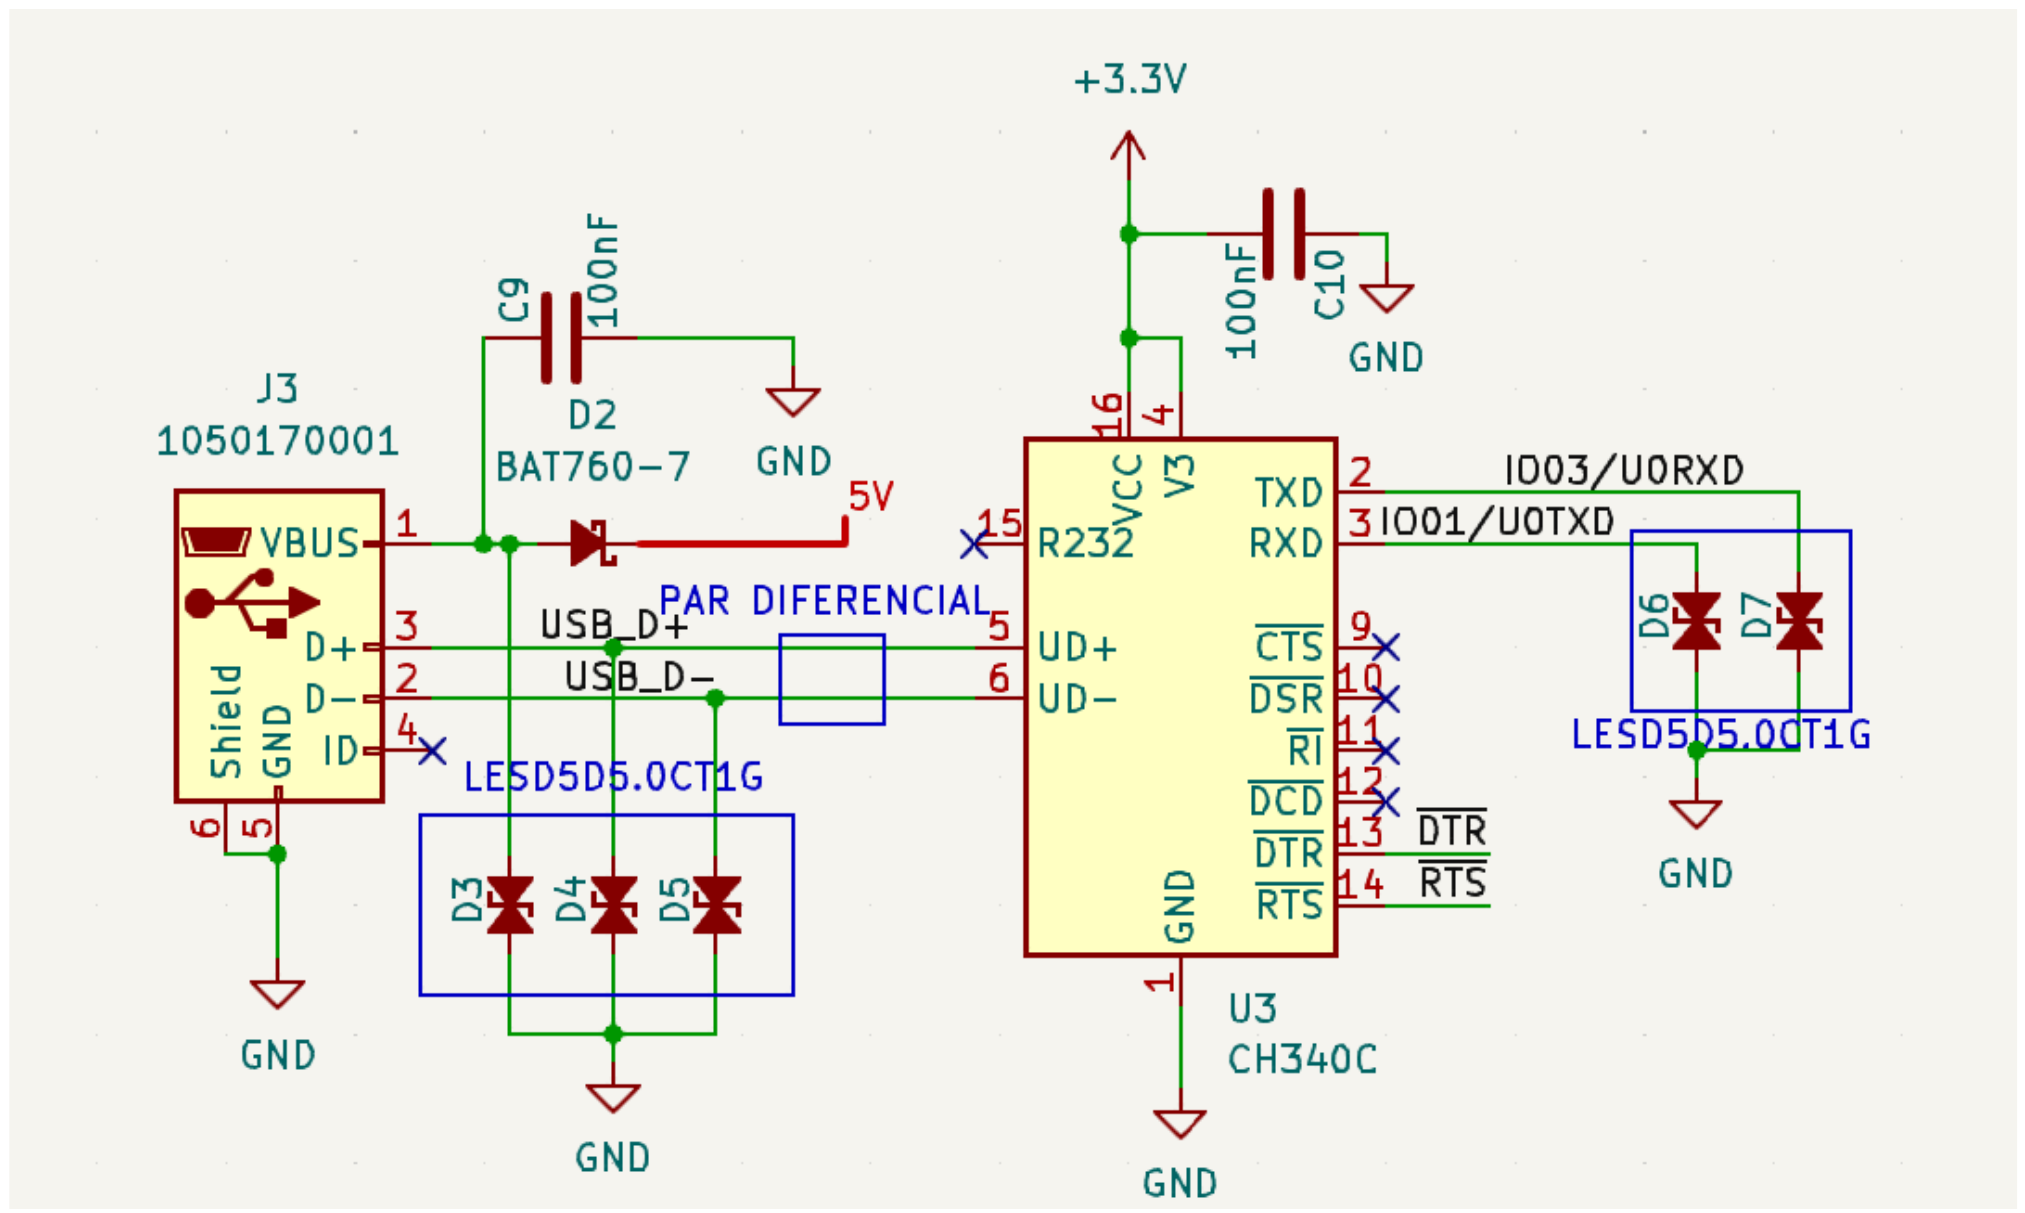
\includegraphics[max width=\linewidth,max height=0.82\textheight]{figuras/figura-60.png}
\label{fig:60}
\caption{Figura 60: Label nas trilhas de comunicação USB com diodos de proteção}
\end{figure}

\begin{figure}[H]
\centering
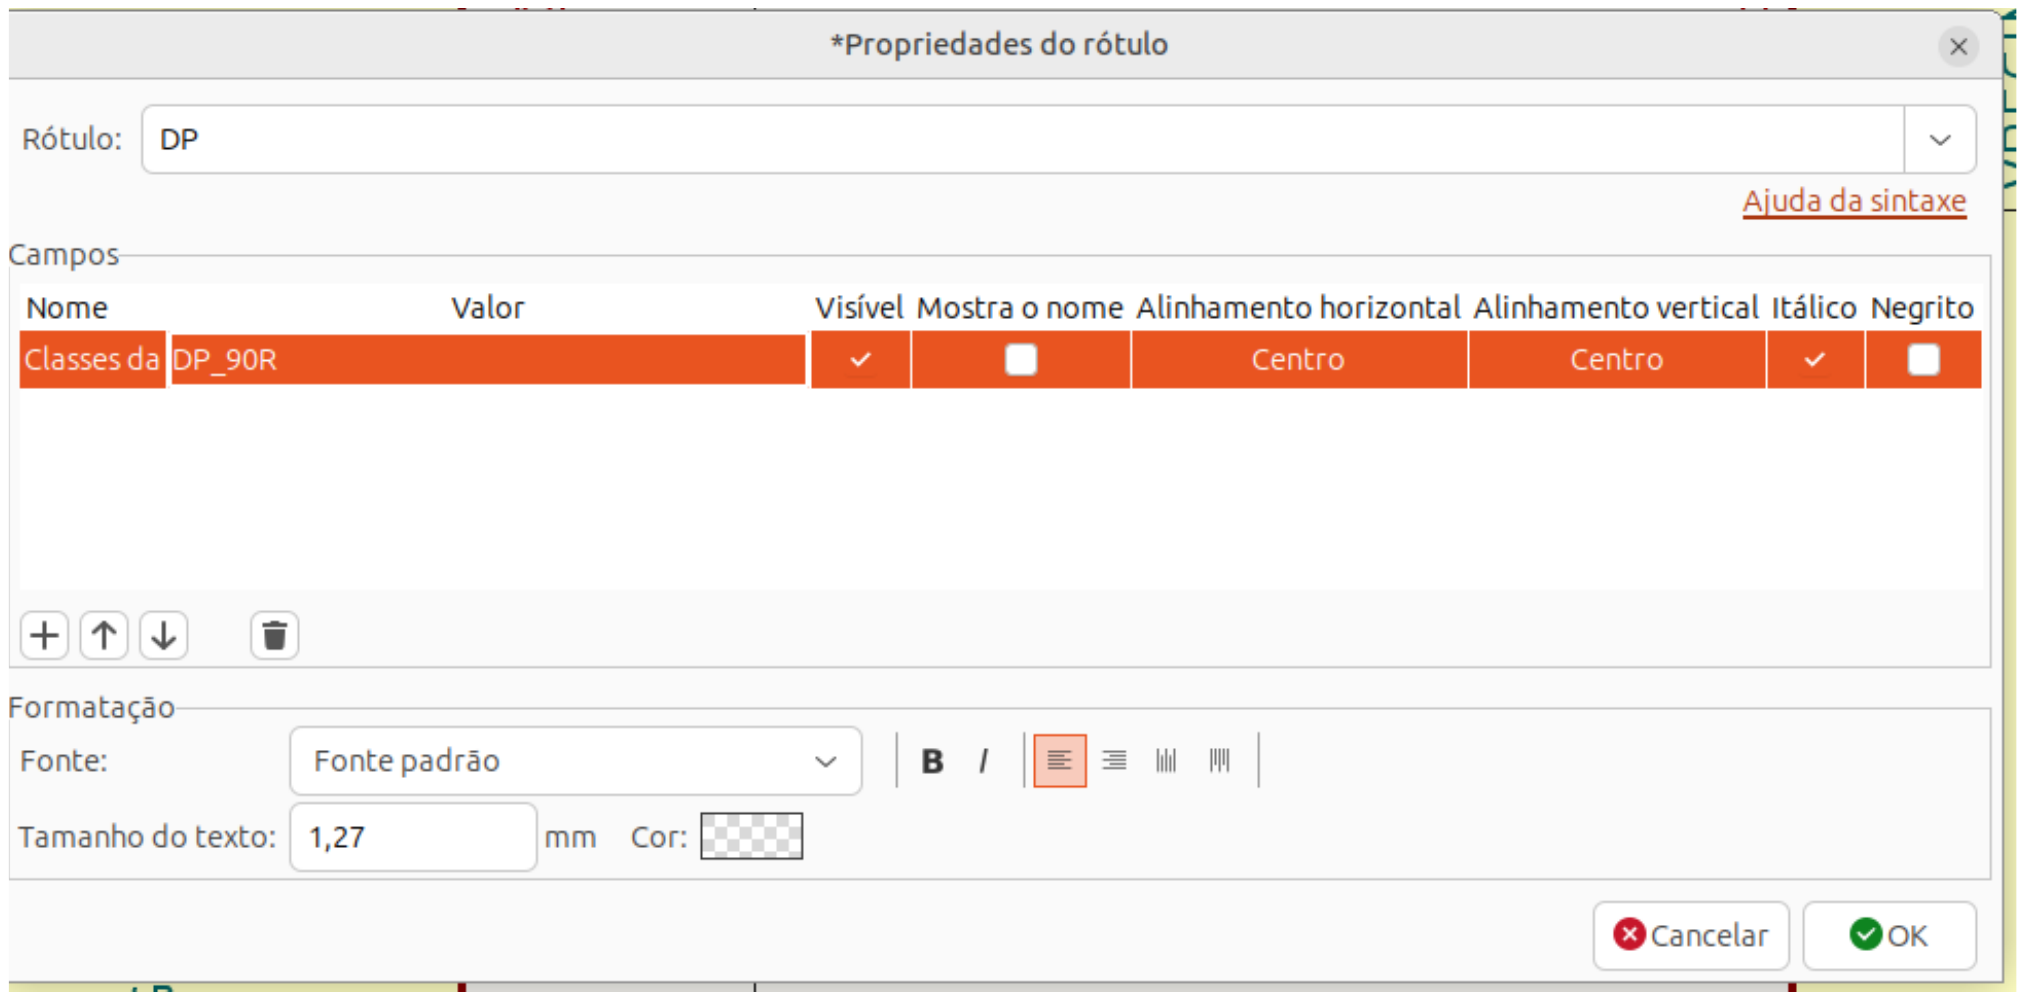
\includegraphics[max width=\linewidth,max height=0.82\textheight]{figuras/figura-61.png}
\label{fig:61}
\caption{Figura 61: Definição dos labels do par diferencial e atribuição a classe DP\_90R}
\end{figure}

\begin{figure}[H]
\centering
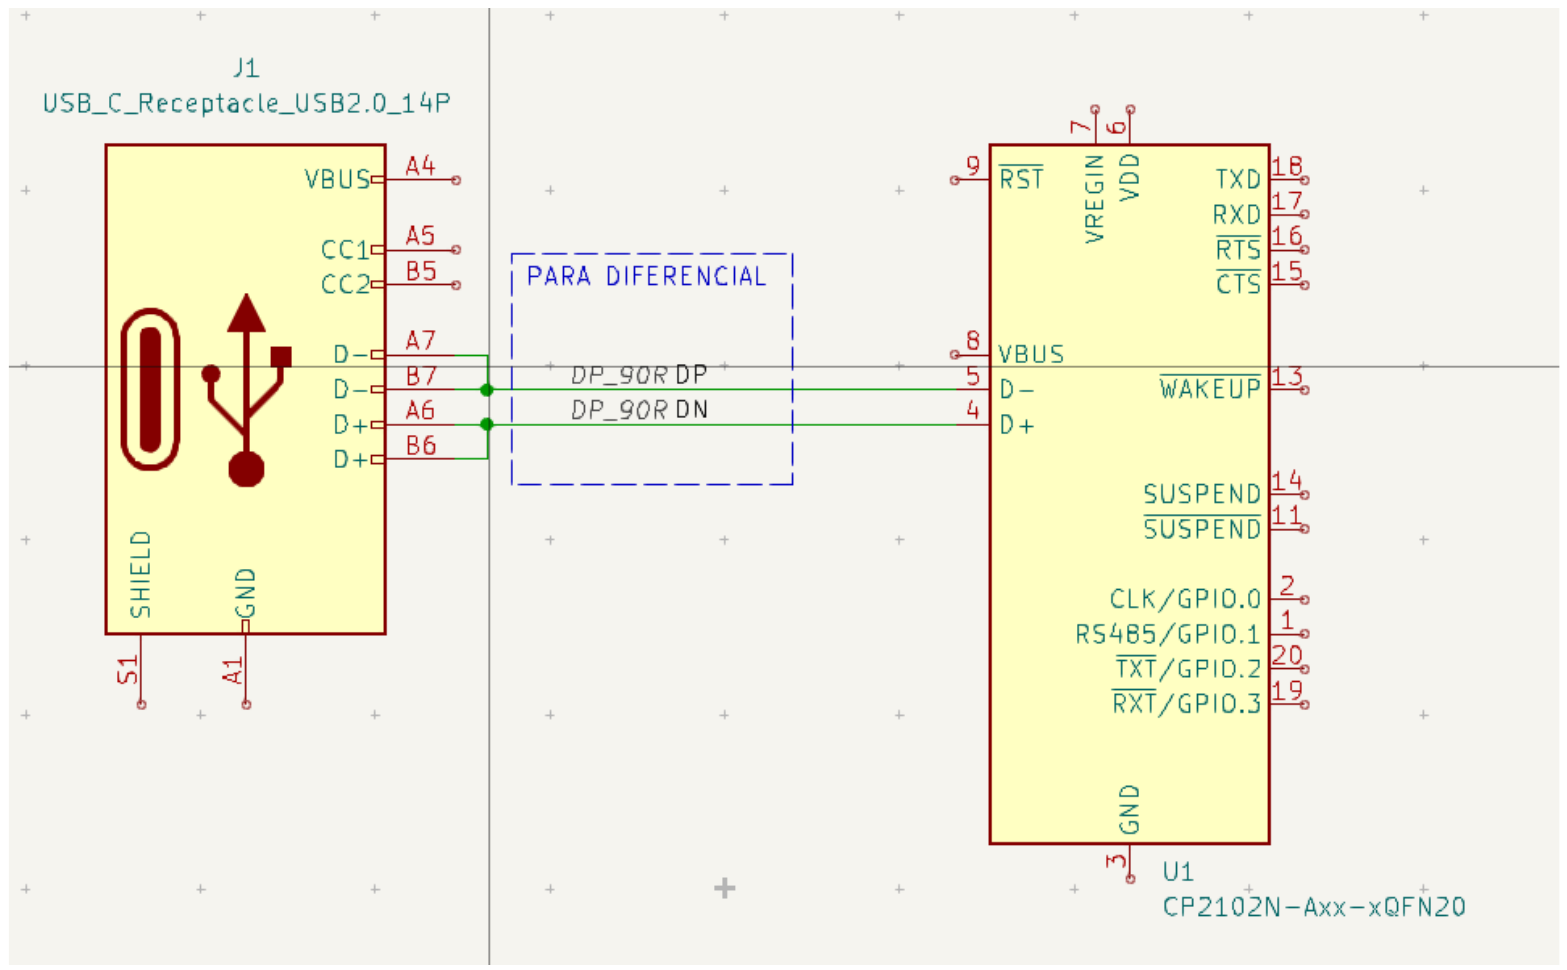
\includegraphics[max width=\linewidth,max height=0.82\textheight]{figuras/figura-62.png}
\label{fig:62}
\caption{Figura 62: Label nas trilhas de comunicação USB sem diodos de proteção}
\end{figure}

controle de impedância. O caso apresentado trata da JLCPCB.

\hypertarget{acesse-httpsjlcpcb.comptimpedance}{%
\subsubsection{\texorpdfstring{Acesse \url{https://jlcpcb.com/pt/impedance}}{Acesse https://jlcpcb.com/pt/impedance}}\label{acesse-httpsjlcpcb.comptimpedance}}

e verifique os parâmetros para multicamada. Os dados contidos nessa página serão importantes para uso posterior. A figura a seguir apresenta os parâmetros para PCB multicamada.

\begin{figure}[H]
\centering
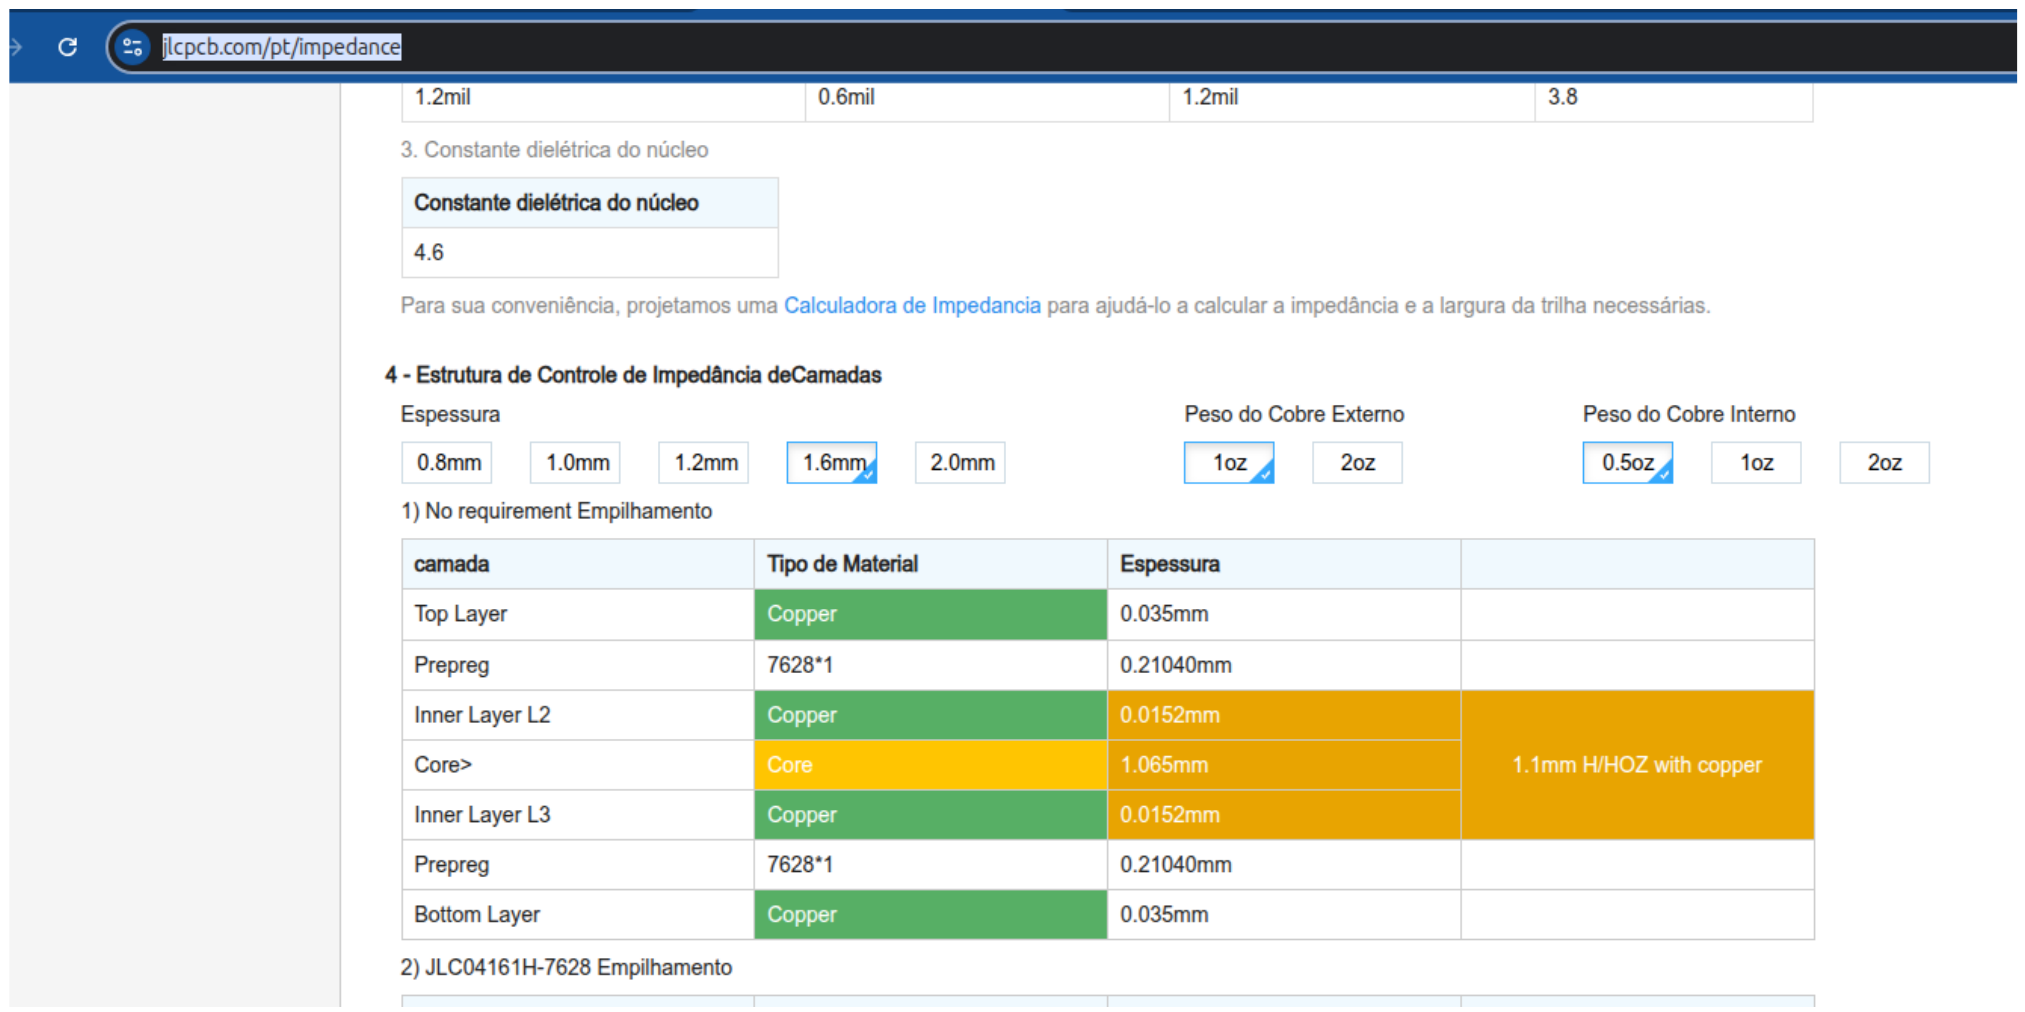
\includegraphics[max width=\linewidth,max height=0.82\textheight]{figuras/figura-63.png}
\label{fig:63}
\caption{Figura 63: Estrutura com parâmetros para o controle de impedância}
\end{figure}

Esses parâmetros devem ser inseridos no KiCAD em configuração da placa conforme a figura a seguir.

\begin{figure}[H]
\centering
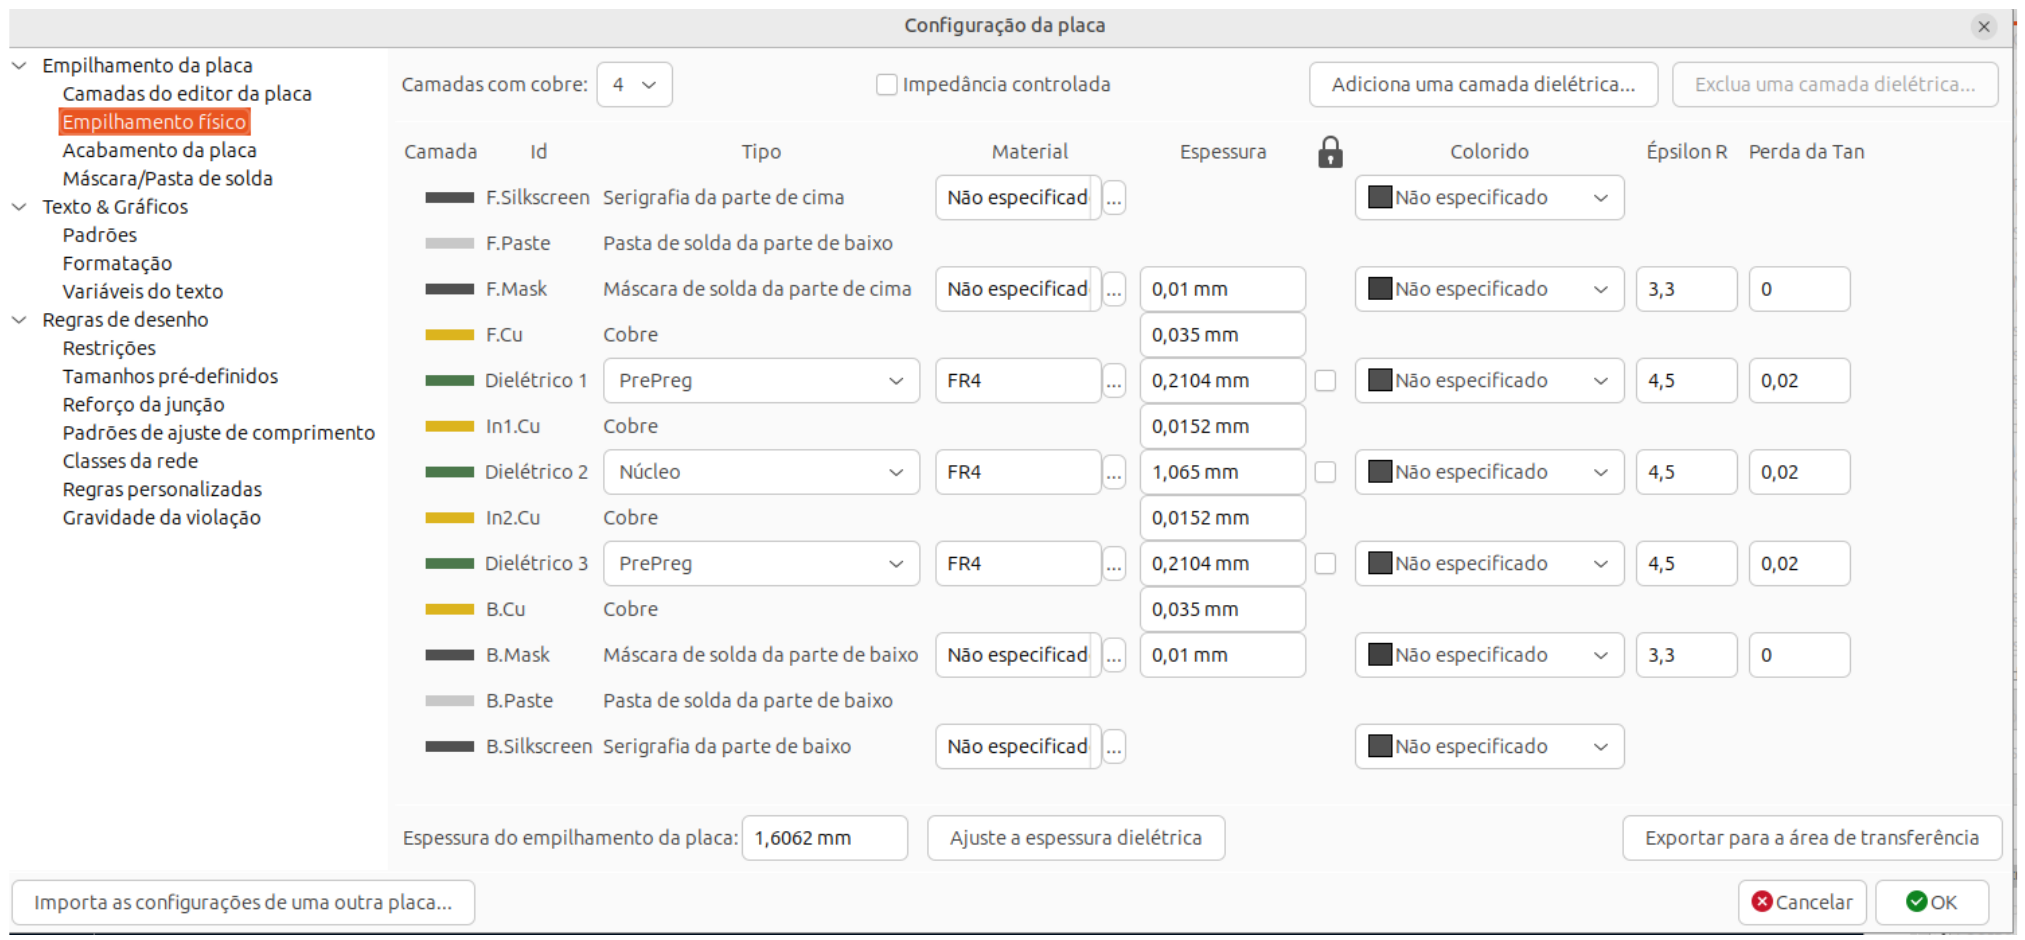
\includegraphics[max width=\linewidth,max height=0.82\textheight]{figuras/figura-64.png}
\label{fig:64}
\caption{Figura 64: Configuração da placa com edição dos parâmetros conforme compatibilidade da JLCPCB}
\end{figure}

Pode-se também realizar o acesso pelo link contido na página de compatibilidades da JLCPCB

\begin{figure}[H]
\centering
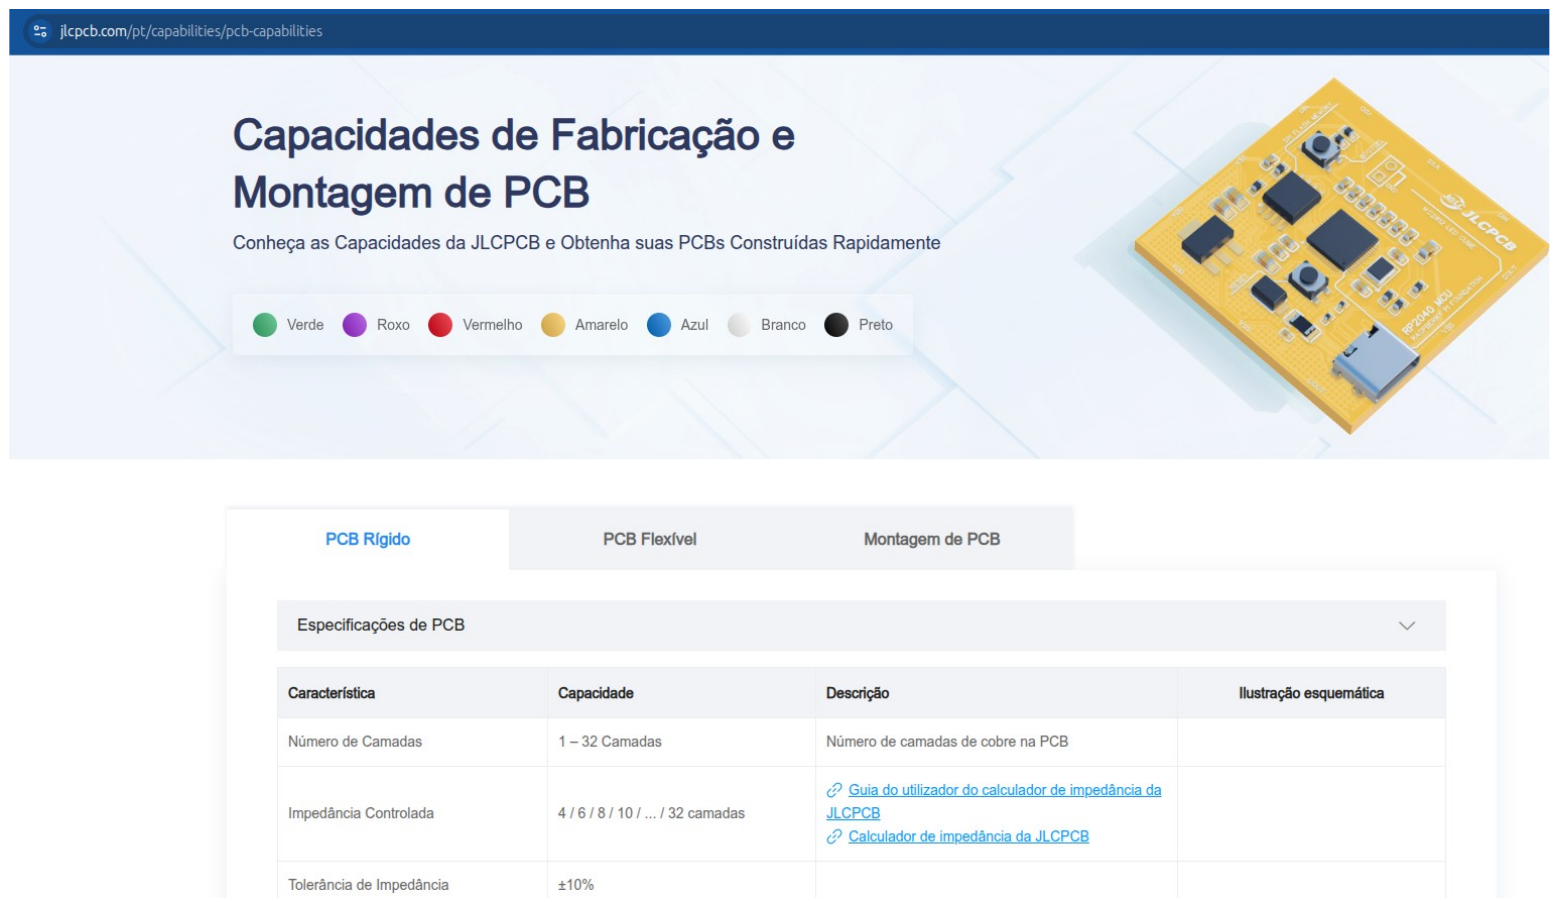
\includegraphics[max width=\linewidth,max height=0.82\textheight]{figuras/figura-65.png}
\label{fig:65}
\caption{Figura 65: Página de compatibilidades da JLCPCB. Link para guia e calculadora de impedância}
\end{figure}

\hypertarget{troque-a-unidade-para-mm.}{%
\subsubsection{Troque a unidade para mm.}\label{troque-a-unidade-para-mm.}}

\begin{figure}[H]
\centering
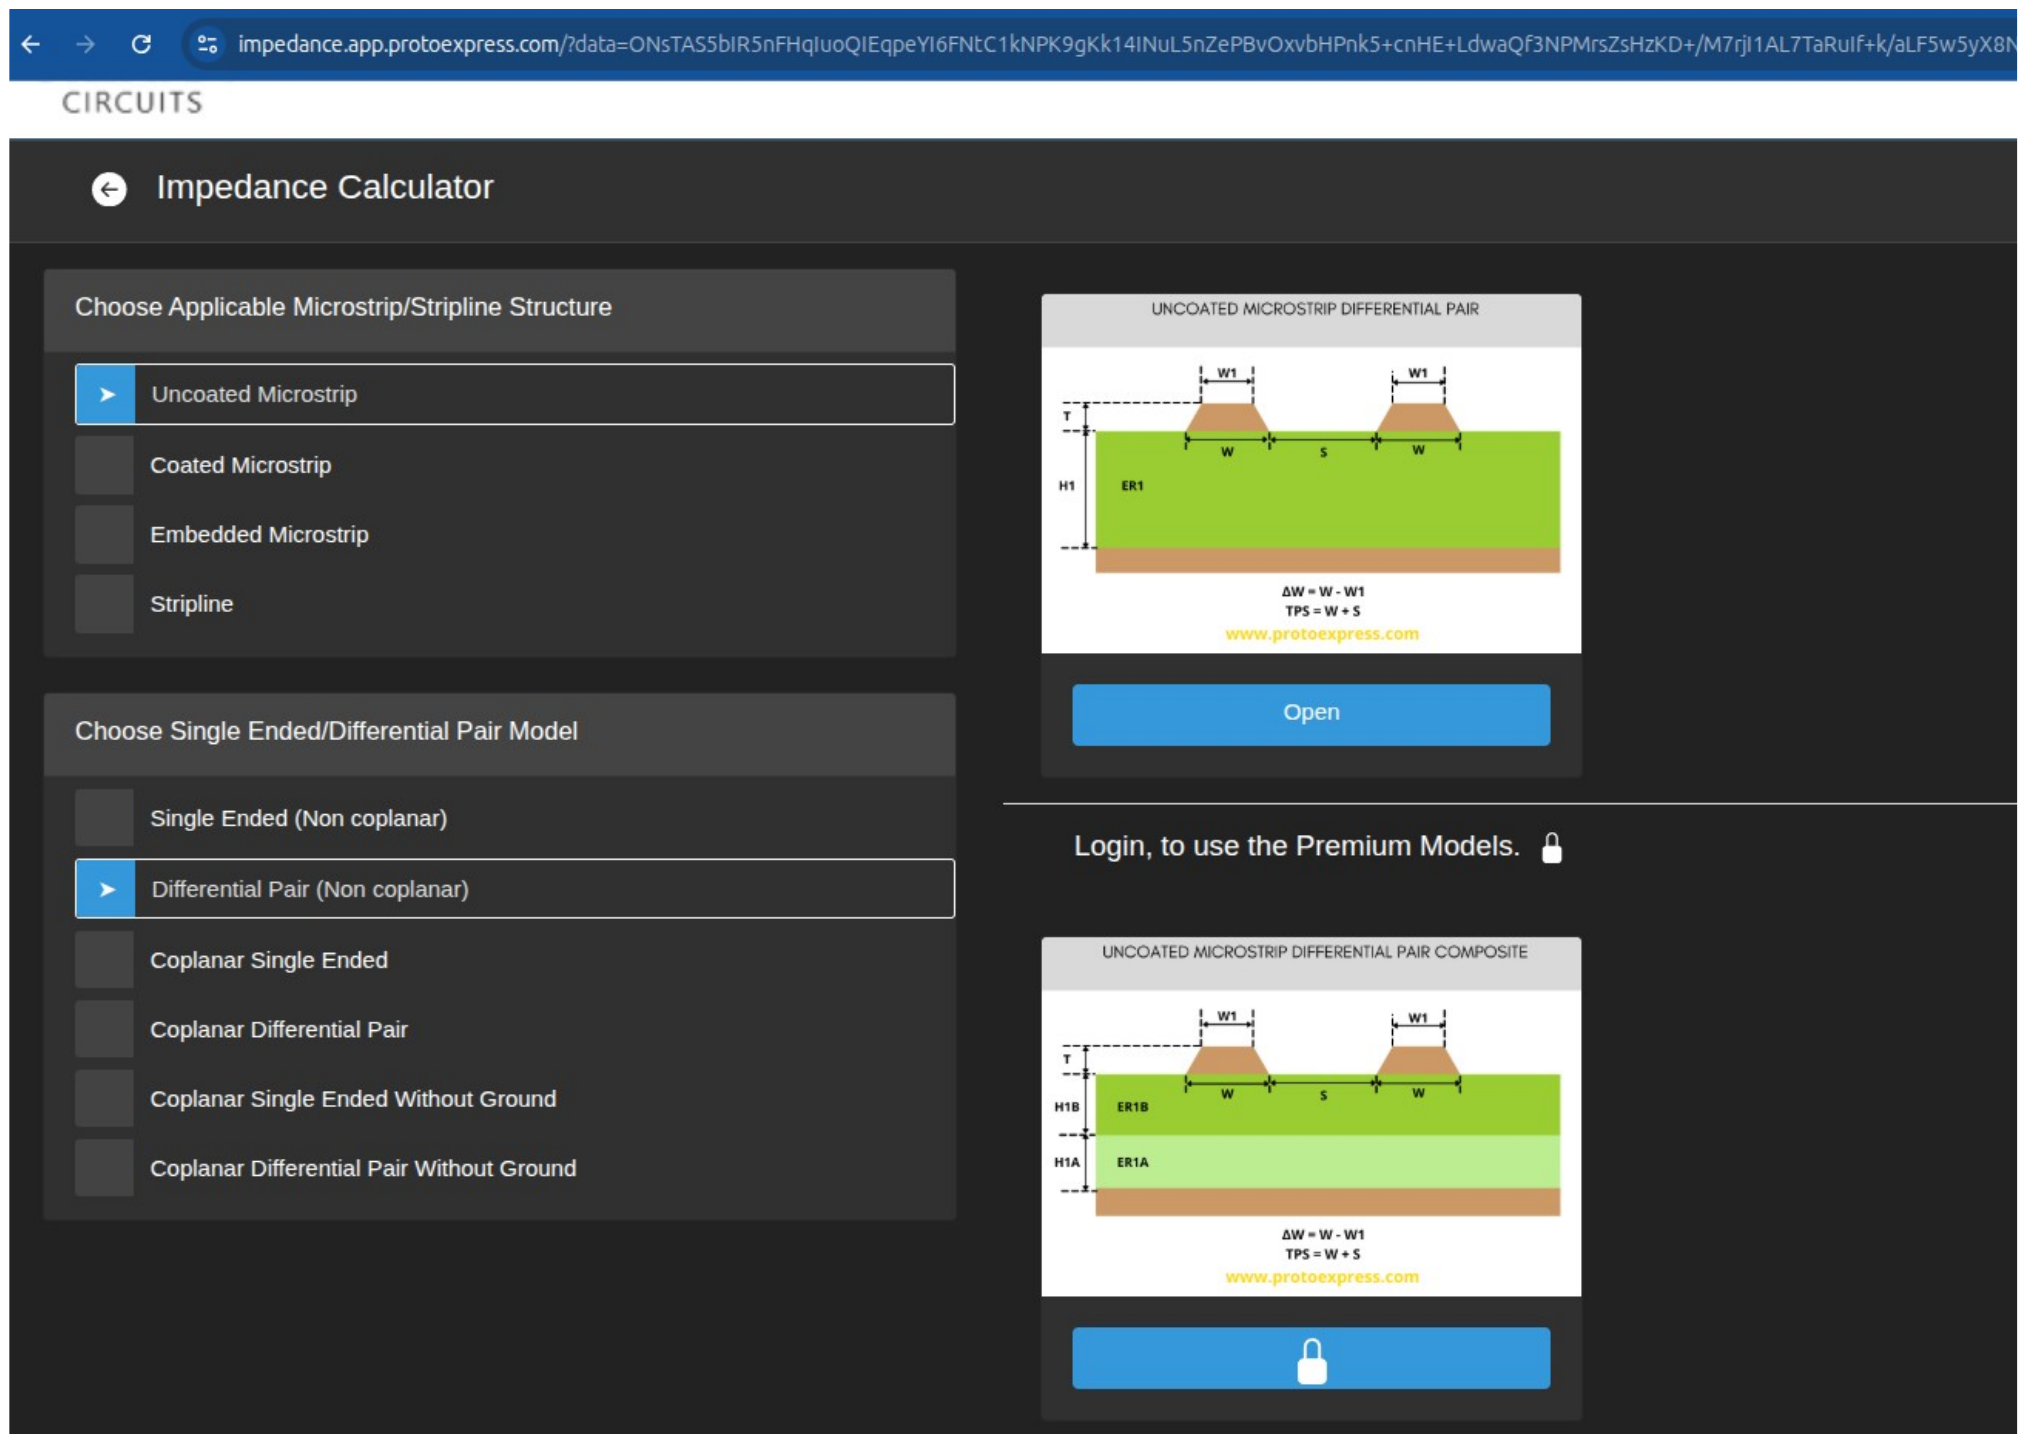
\includegraphics[max width=\linewidth,max height=0.82\textheight]{figuras/figura-66.png}
\label{fig:66}
\caption{Figura 66: Trilhas não revestidas (uncoated) par diferencial}
\end{figure}

No site da JLCPCB, na página de controle de impedância, obtenha a constante dielétrica do material prepreg 7628, que corresponde a 4,4.

\begin{figure}[H]
\centering
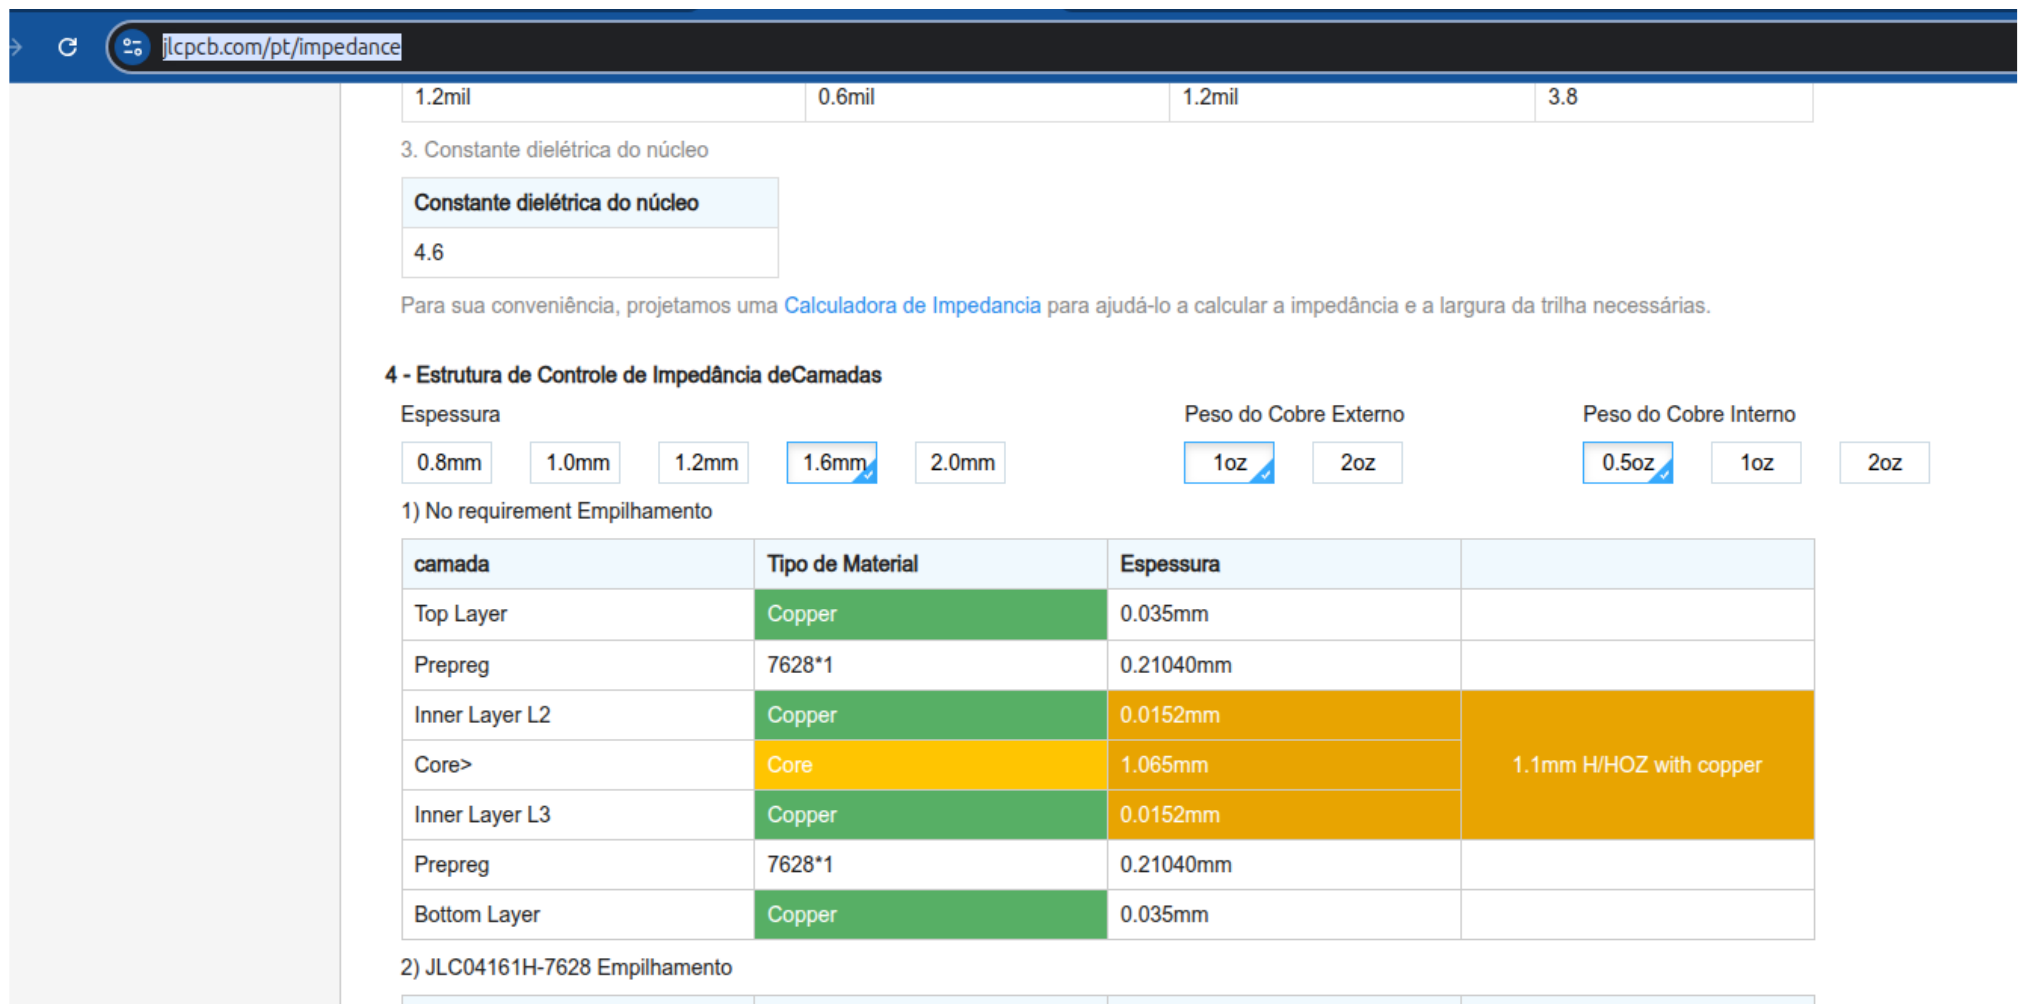
\includegraphics[max width=\linewidth,max height=0.82\textheight]{figuras/figura-67.png}
\label{fig:67}
\caption{Figura 67: Estrutura com parâmetros para o controle de impedância}
\end{figure}

\begin{figure}[H]
\centering
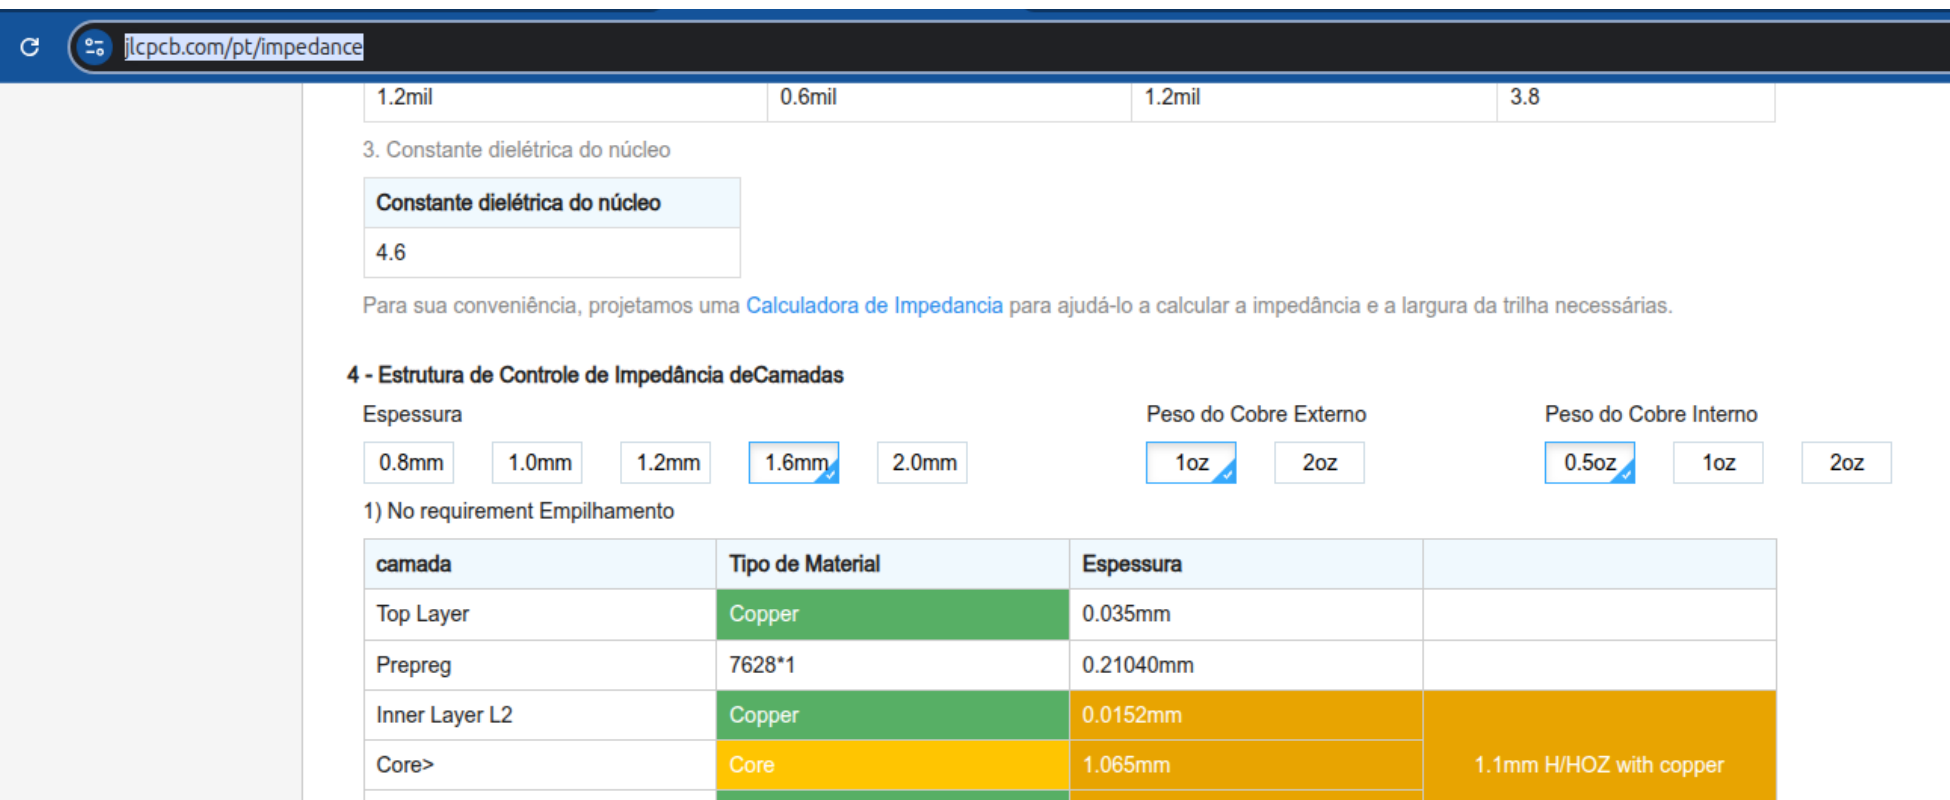
\includegraphics[max width=\linewidth,max height=0.82\textheight]{figuras/figura-68.png}
\label{fig:68}
\caption{Figura 68: Constantes dielétricas obtidas nas páginas de controle de impedância do JLCPCB}
\end{figure}

Além da constante dielétrica obtenha a altura do material prepreg 7628 (0,21040 mm) conforme a figura anterior. Inclua na calculadora a distância entre trilhas (0,2 mm em Trace Separation (S) ( mm )) valor obtido na configuração da placa classe de rede DP\_90R.

\begin{figure}[H]
\centering
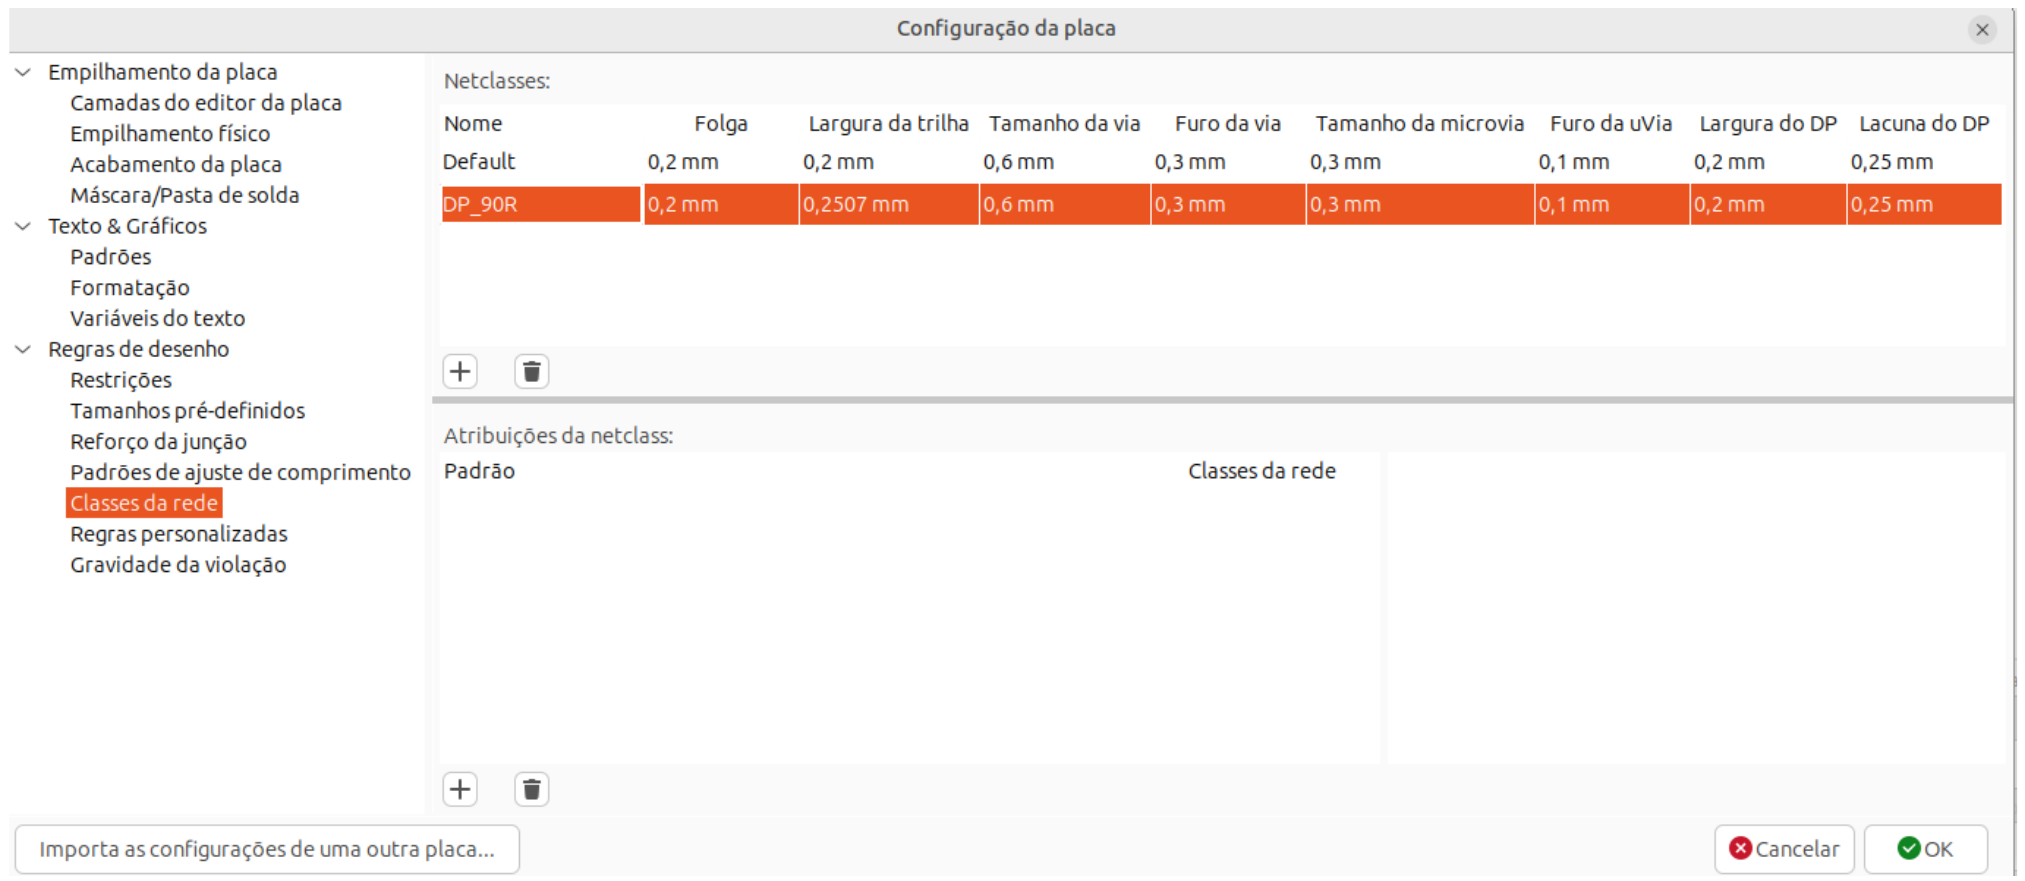
\includegraphics[max width=\linewidth,max height=0.82\textheight]{figuras/figura-69.png}
\label{fig:69}
\caption{Figura 69: Parâmetros da classe DP\_90R}
\end{figure}

Insira o valor de 90 ohms para a impedância alvo. Outros tipos de barramento possuem impedâncias próprias.

\begin{figure}[H]
\centering
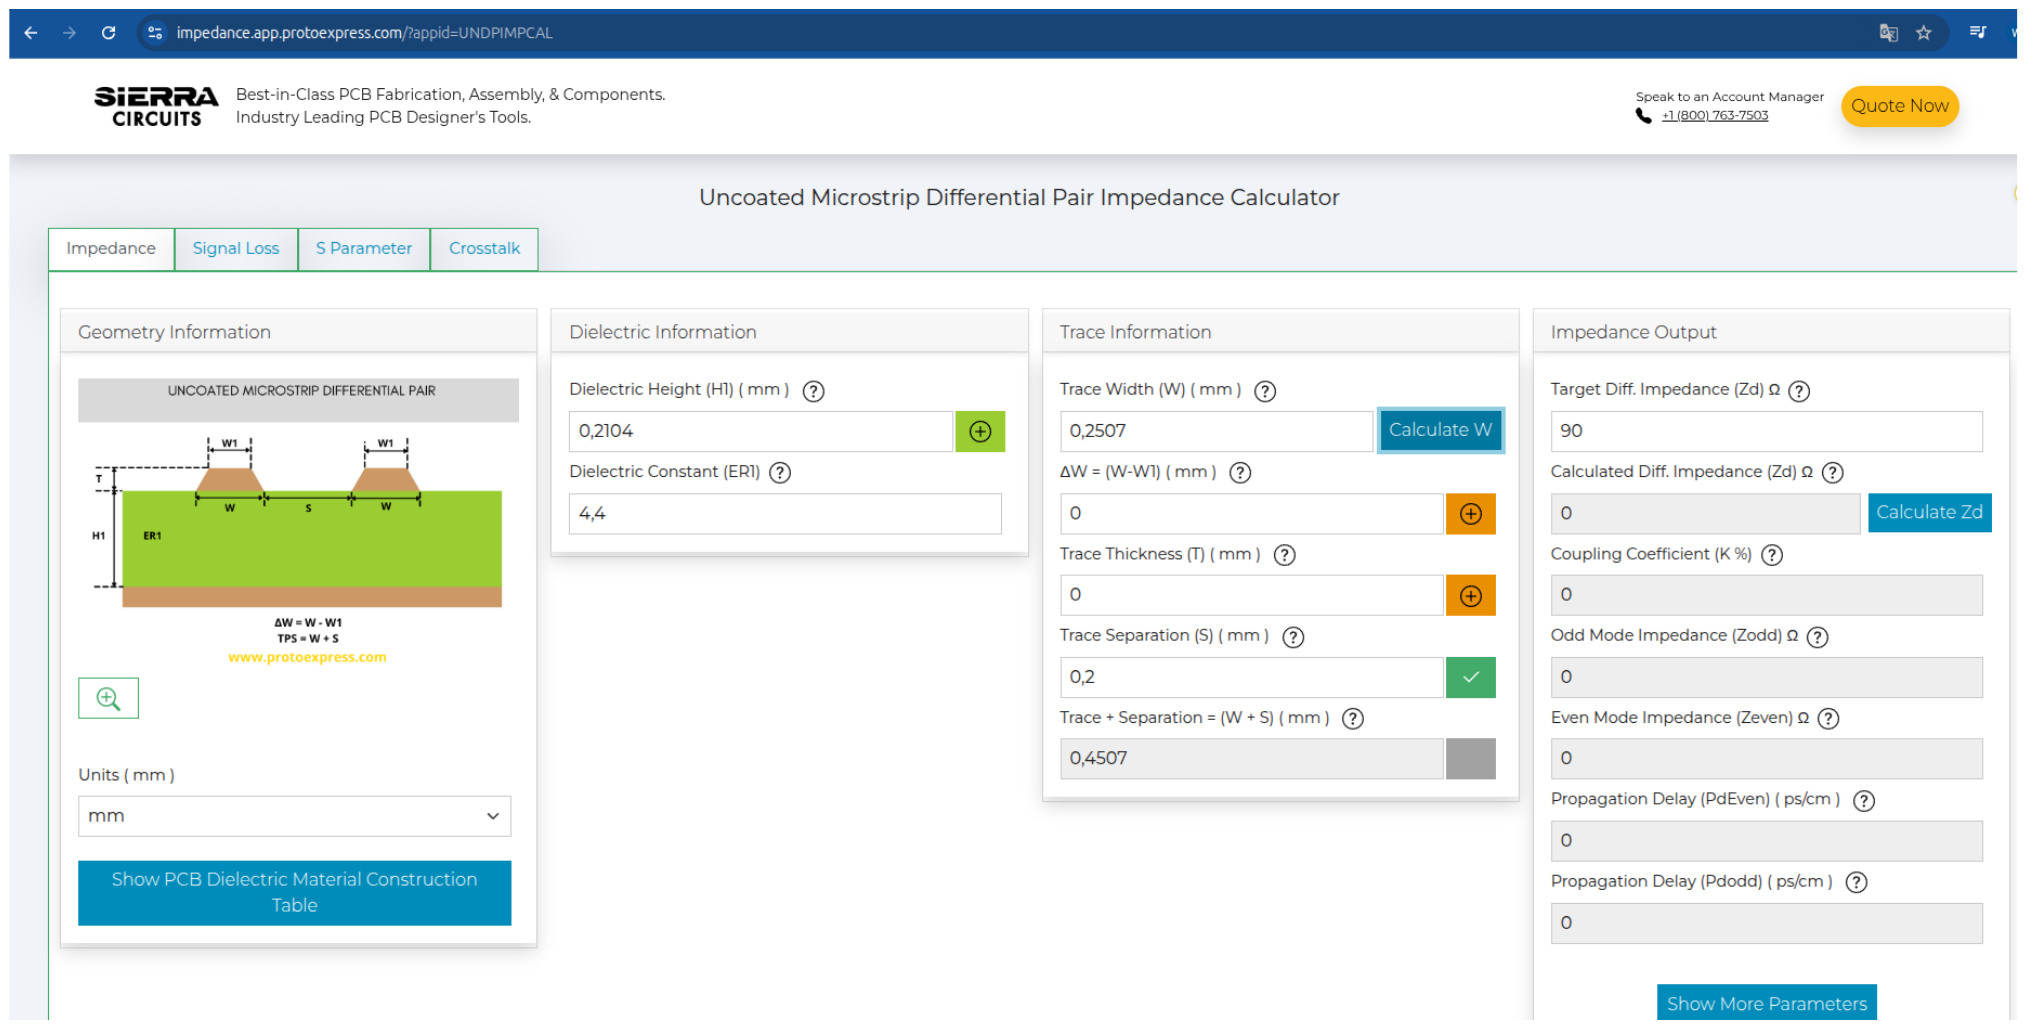
\includegraphics[max width=\linewidth,max height=0.82\textheight]{figuras/figura-70.png}
\label{fig:70}
\caption{Figura 70: Calculadora de impedância da Sierra Circuits}
\end{figure}

Após selecionar a unidade para mm, preencher os parâmetros:

\hypertarget{altura-do-dieluxe9trico-02104-mm}{%
\subsubsection{Altura do dielétrico: 0,2104 mm}\label{altura-do-dieluxe9trico-02104-mm}}

Constante dielétrica para o material prepreg 7628: 4,4

\hypertarget{separauxe7uxe3o-entre-trilhas-02-mm}{%
\subsubsection{Separação entre trilhas: 0,2 mm}\label{separauxe7uxe3o-entre-trilhas-02-mm}}

\hypertarget{impeduxe2ncia-alvo-90-ohms}{%
\subsubsection{Impedância alvo: 90 ohms}\label{impeduxe2ncia-alvo-90-ohms}}

Clique em \textbf{Calcular W} e será obtido o valor da largura da trilha.

Insira o valor calculado da trilha na classe DP\_90R conforme a figura.

\begin{figure}[H]
\centering
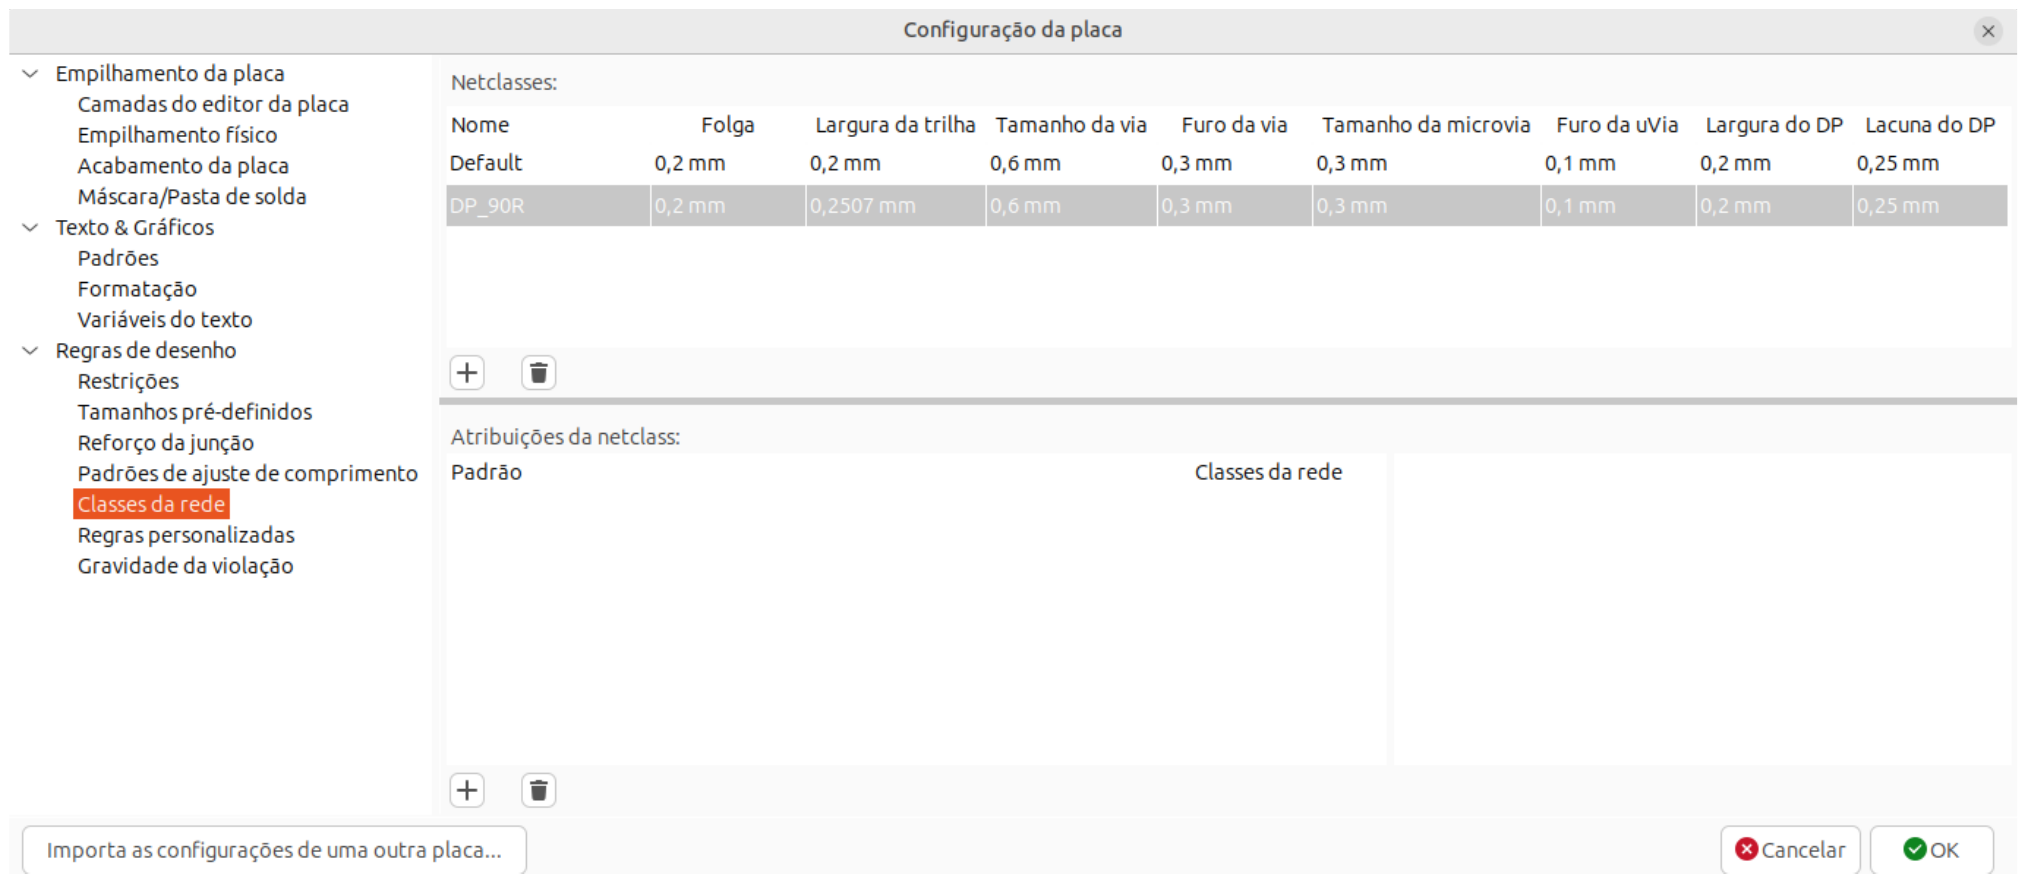
\includegraphics[max width=\linewidth,max height=0.82\textheight]{figuras/figura-71.png}
\label{fig:71}
\caption{Figura 71: Largura da trilha para a classe DP\_90R}
\end{figure}

\begin{figure}[H]
\centering
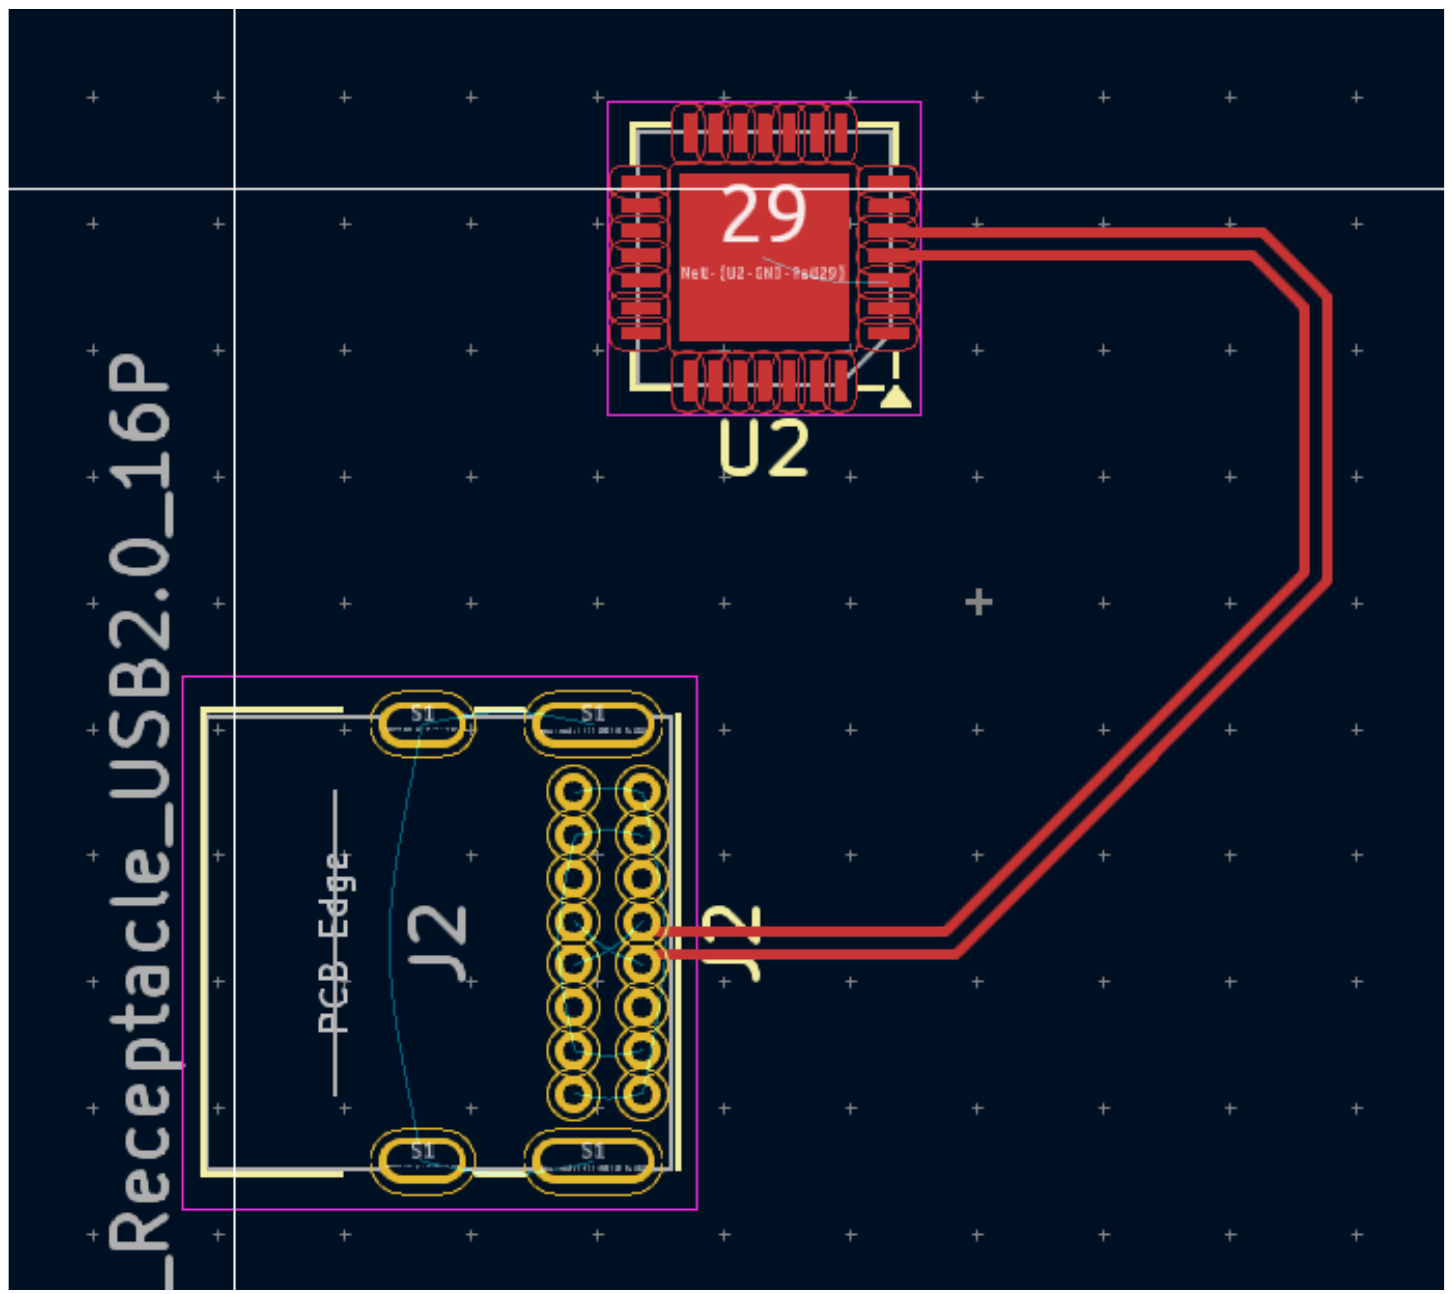
\includegraphics[max width=\linewidth,max height=0.82\textheight]{figuras/figura-72.png}
\label{fig:72}
\caption{Figura 72: Roteamento do par diferencial}
\end{figure}

Devido a geometria das trilhas do par diferencial, mas mesmas não possuem o mesmo comprimento. Logo, será necessário realizar alguns ajustes para garantir que os sinais elétricos sejam recebidos no mesmo tempo.

Se houver uma diferença de comprimento (ou atraso), chamada de \textbf{skew}, isso pode causar:

\begin{itemize}
\tightlist
\item
  Jitter (variação temporal) no sinal.
\item
  Degradação da imunidade a ruído (o modo comum não é cancelado corretamente).
\item
  Erros de comunicação em altas frequências. Verifique o comprimento de cada trilha, para isso use \textbf{a tecla de atalho ``7''.}
  \par\noindent\makebox[\linewidth][c]{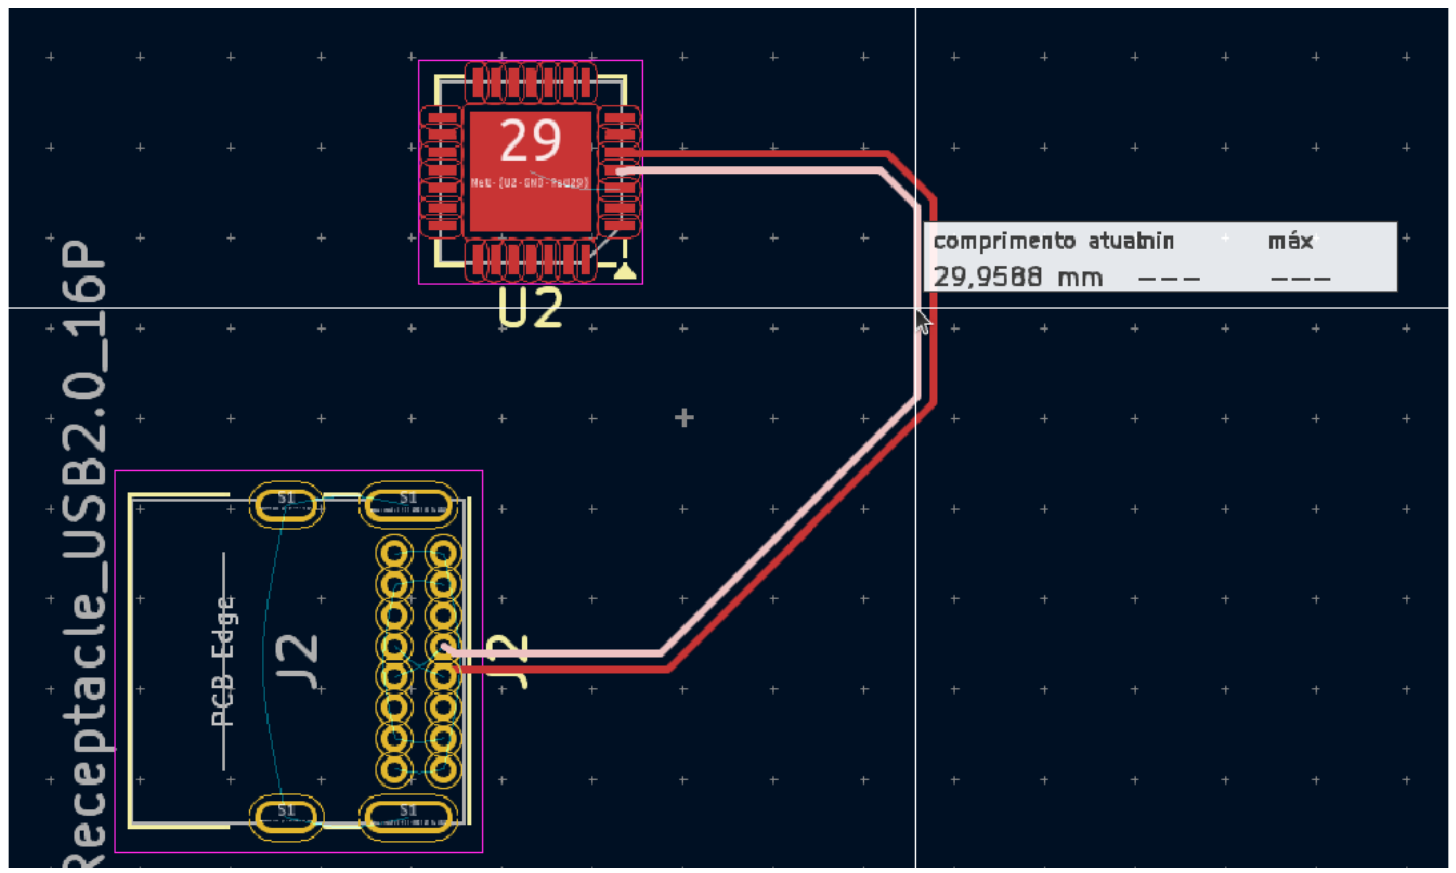
\includegraphics[max width=\linewidth,max height=0.82\textheight]{figuras/figura-73.png}}\par\label{fig:73}
\end{itemize}

\begin{figure}[H]
\centering
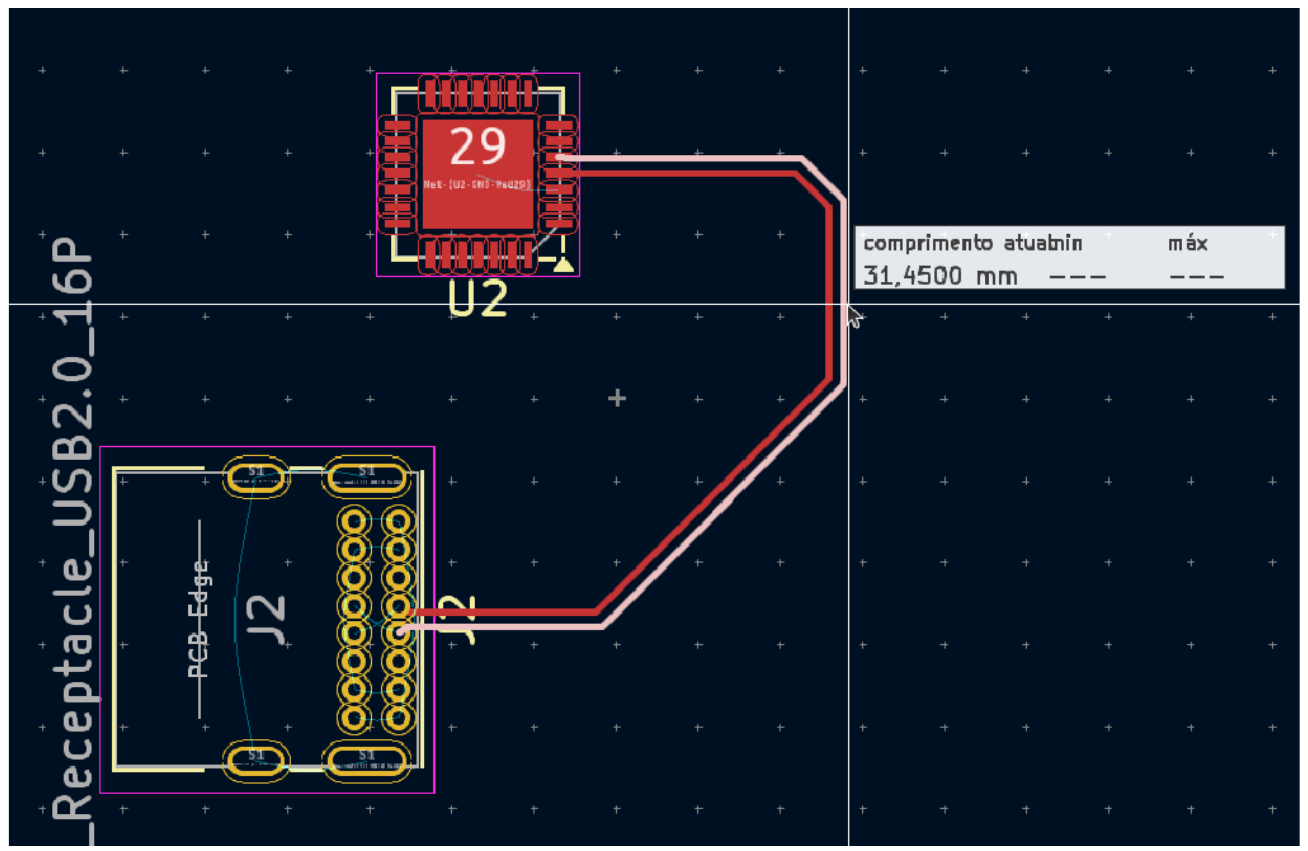
\includegraphics[max width=\linewidth,max height=0.82\textheight]{figuras/figura-74.png}
\label{fig:74}
\caption{Figura 74: Comprimento da trilha do par diferencial}
\end{figure}

Conforme as figuras anteriores, pode-se observar que as trilhas possuem comprimentos de 31,45 mm e 29,9588 mm. Deve-se preceder com os ajuste de comprimento para equalização.

Use a \textbf{tecla de atalho ``8''}, para clique com o botão direito do mouse na maior trilha e selecione \textbf{\emph{Configurações do ajuste de comprimento}}. Observe a figura a seguir.

\begin{figure}[H]
\centering
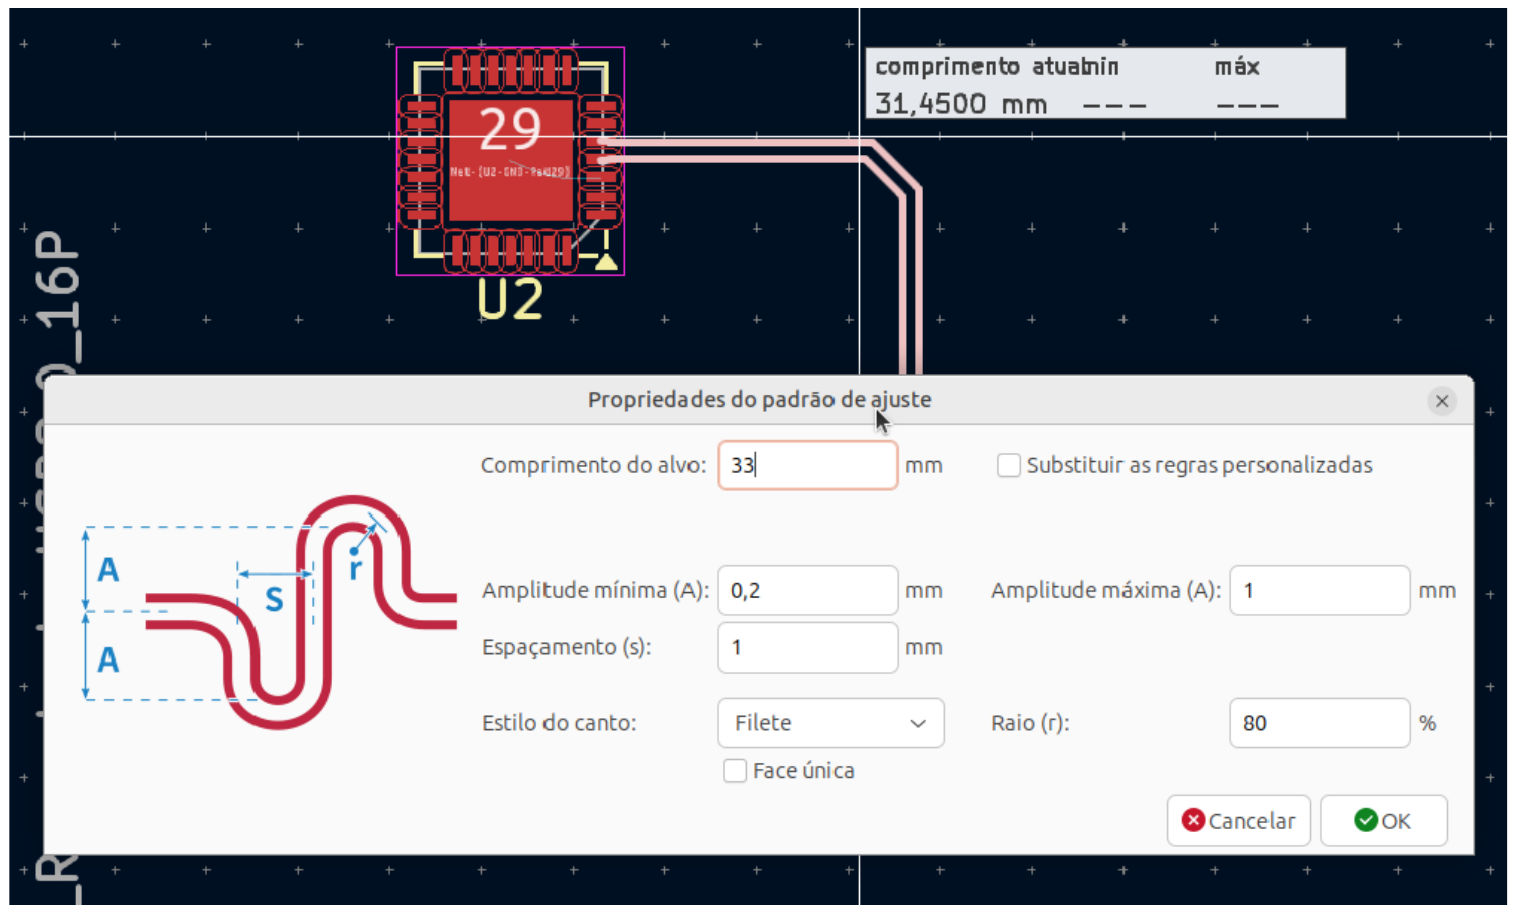
\includegraphics[max width=\linewidth,max height=0.82\textheight]{figuras/figura-75.png}
\label{fig:75}
\caption{Figura 75: Ajuste do comprimento desejado}
\end{figure}

Defina o comprimento alvo igual o comprimento da maior trilha ou pouco superior, no exemplo o valor é de 33 mm.

\begin{figure}[H]
\centering
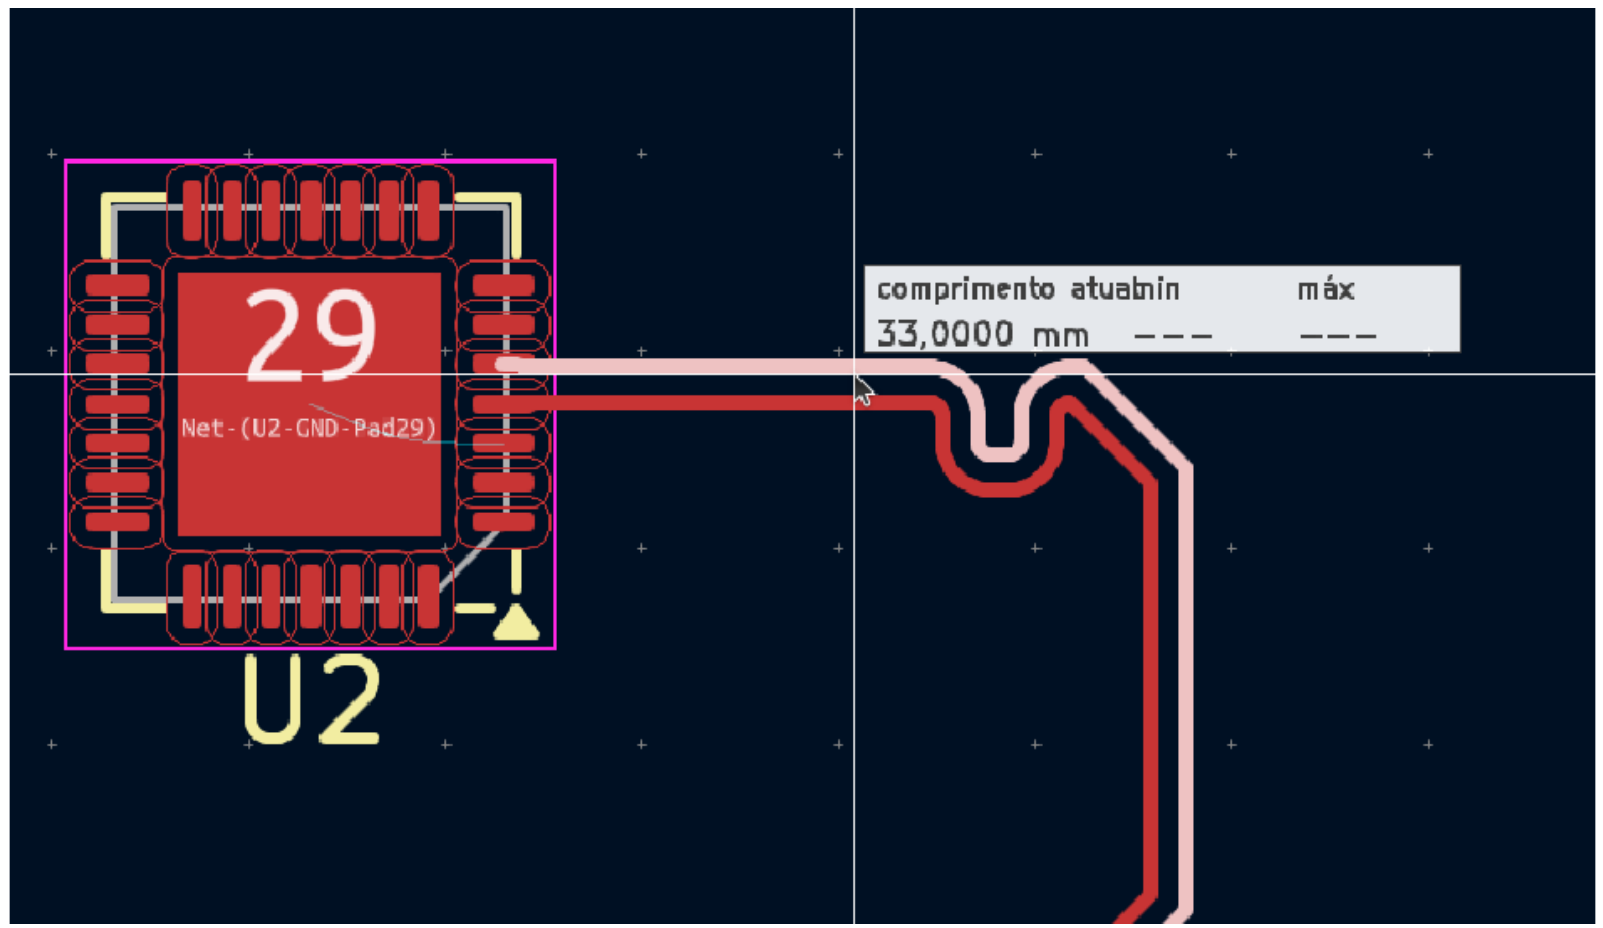
\includegraphics[max width=\linewidth,max height=0.82\textheight]{figuras/figura-76.png}
\label{fig:76}
\caption{Figura 76: Maior trilha com comprimento 33}
\end{figure}

A tecla de atalho 7 deverá ser usada para o ajuste de comprimento da outra trilha.

\begin{figure}[H]
\centering
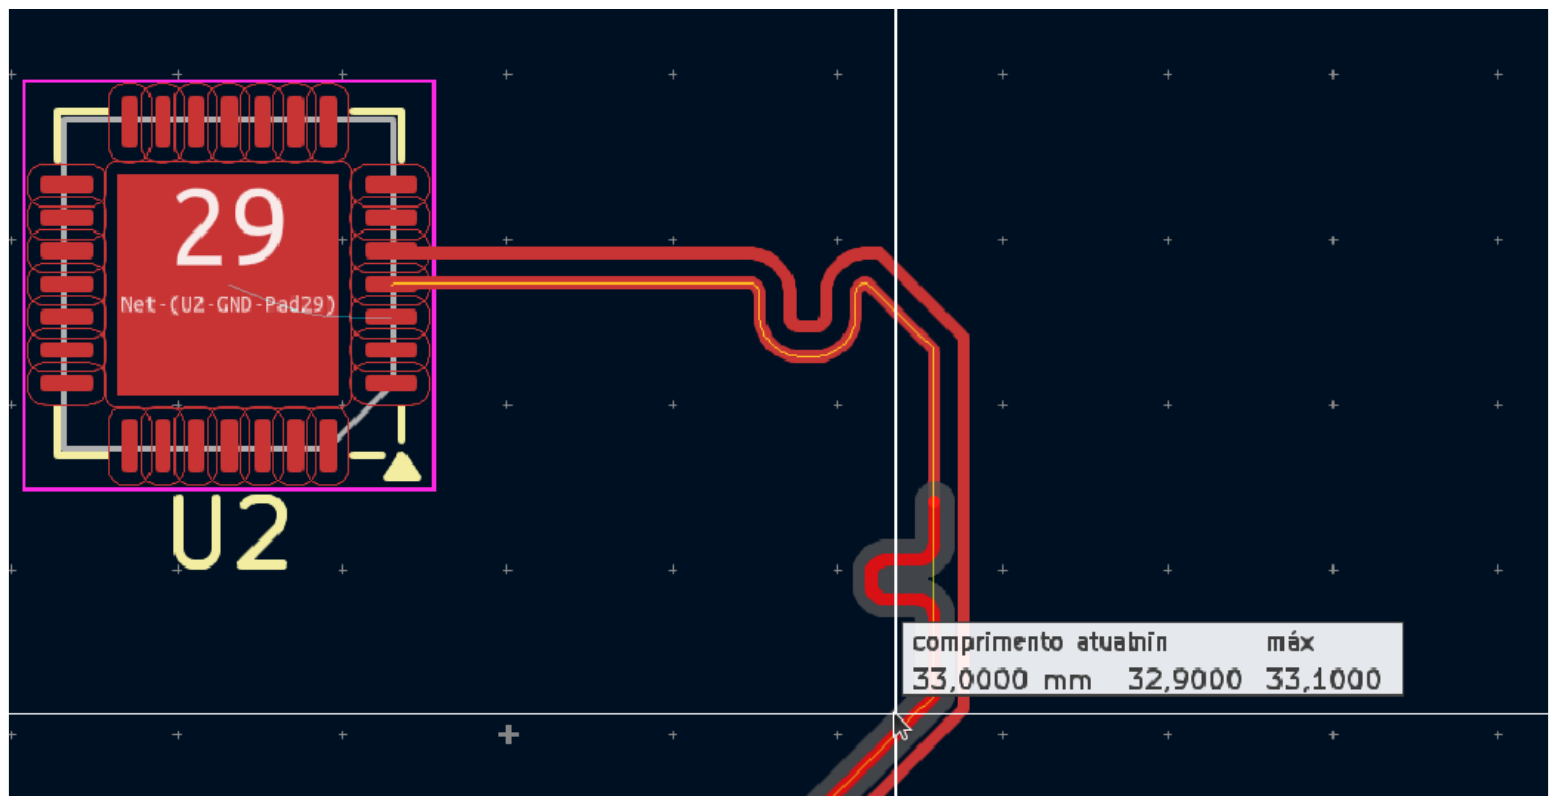
\includegraphics[max width=\linewidth,max height=0.82\textheight]{figuras/figura-77.png}
\label{fig:77}
\caption{Figura 77: Ajuste de comprimento da trilha}
\end{figure}

A figura a seguir apresenta resultado final cujo comprimento de cada trilha é de 33mm.

\begin{figure}[H]
\centering
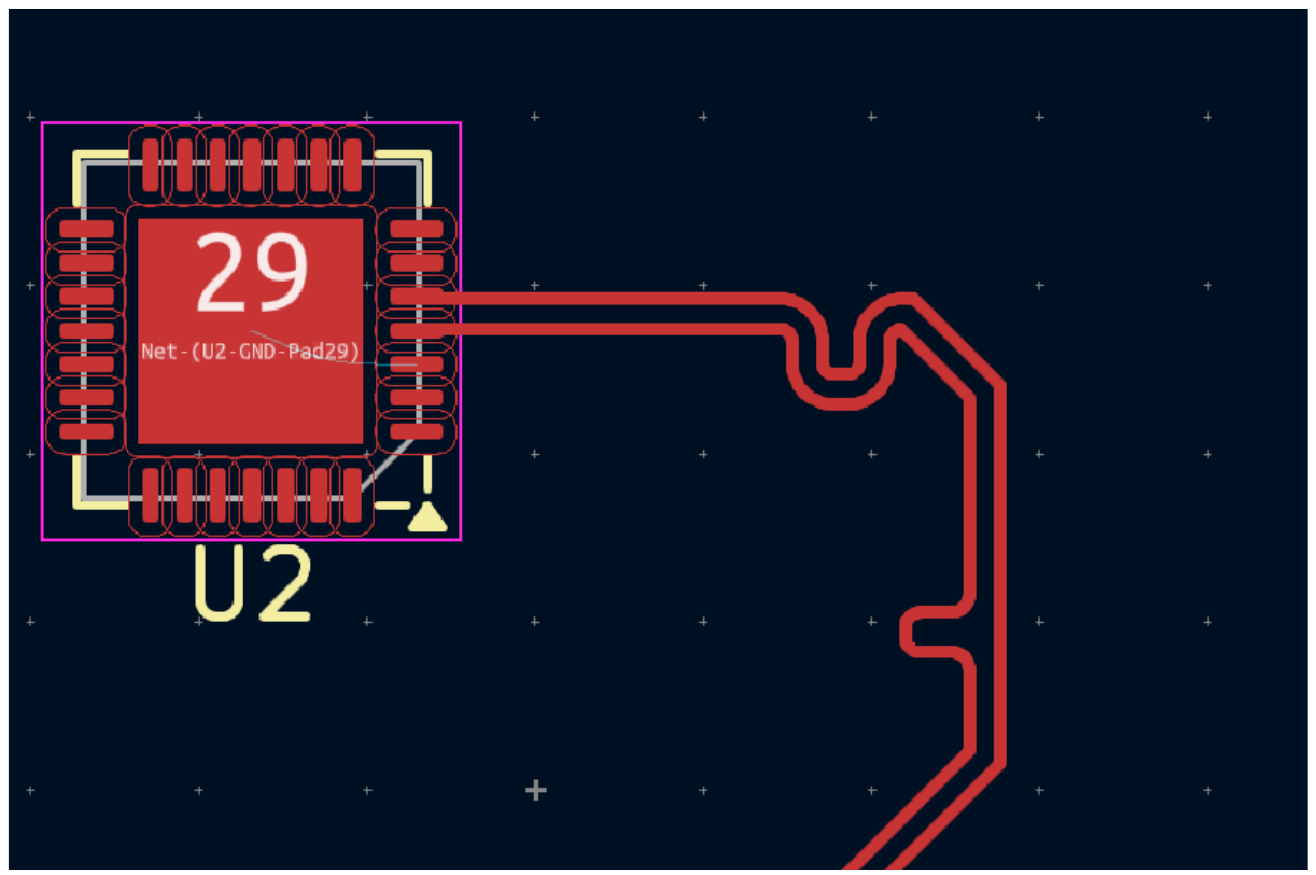
\includegraphics[max width=\linewidth,max height=0.82\textheight]{figuras/figura-78.png}
\label{fig:78}
\caption{Figura 78: Trilhas par diferencial com comprimentos iguais e impedância ajustada}
\end{figure}

\hypertarget{circuitos-para-interfaceamento-de-entrada-e-sauxedda-digital-com-microcontrolador}{%
\chapter{Circuitos para interfaceamento de entrada e saída digital com microcontrolador}\label{circuitos-para-interfaceamento-de-entrada-e-sauxedda-digital-com-microcontrolador}}

As entradas e saídas digitais atuam como interface entre o MCU e os transdutores ou atuadores no campo. Há diversas formas de projetar os circuitos de entrada e saída, adaptáveis aos diferentes sinais utilizados.

\hypertarget{entradas-digitais-em-c.c.}{%
\section{Entradas digitais em C.C.}\label{entradas-digitais-em-c.c.}}

Detectam e convertem sinais de comutação de entrada em níveis lógicos de tensão usados na porta digital do MCU. Os módulos de entradas e saídas digitais podem ser projetados para trabalhar tanto com sinais de tensão contínua, quanto sinais alternados. Para os níveis de C.C., o padrão industrial adotado é de 24 V, o qual possui uma relação sinal/ruído adequada para ambientes industriais e 110 e 220 V, para níveis CA. A figura a seguir apresenta um exemplo esquemático para sinal da entrada digital.

\begin{figure}[H]
\centering
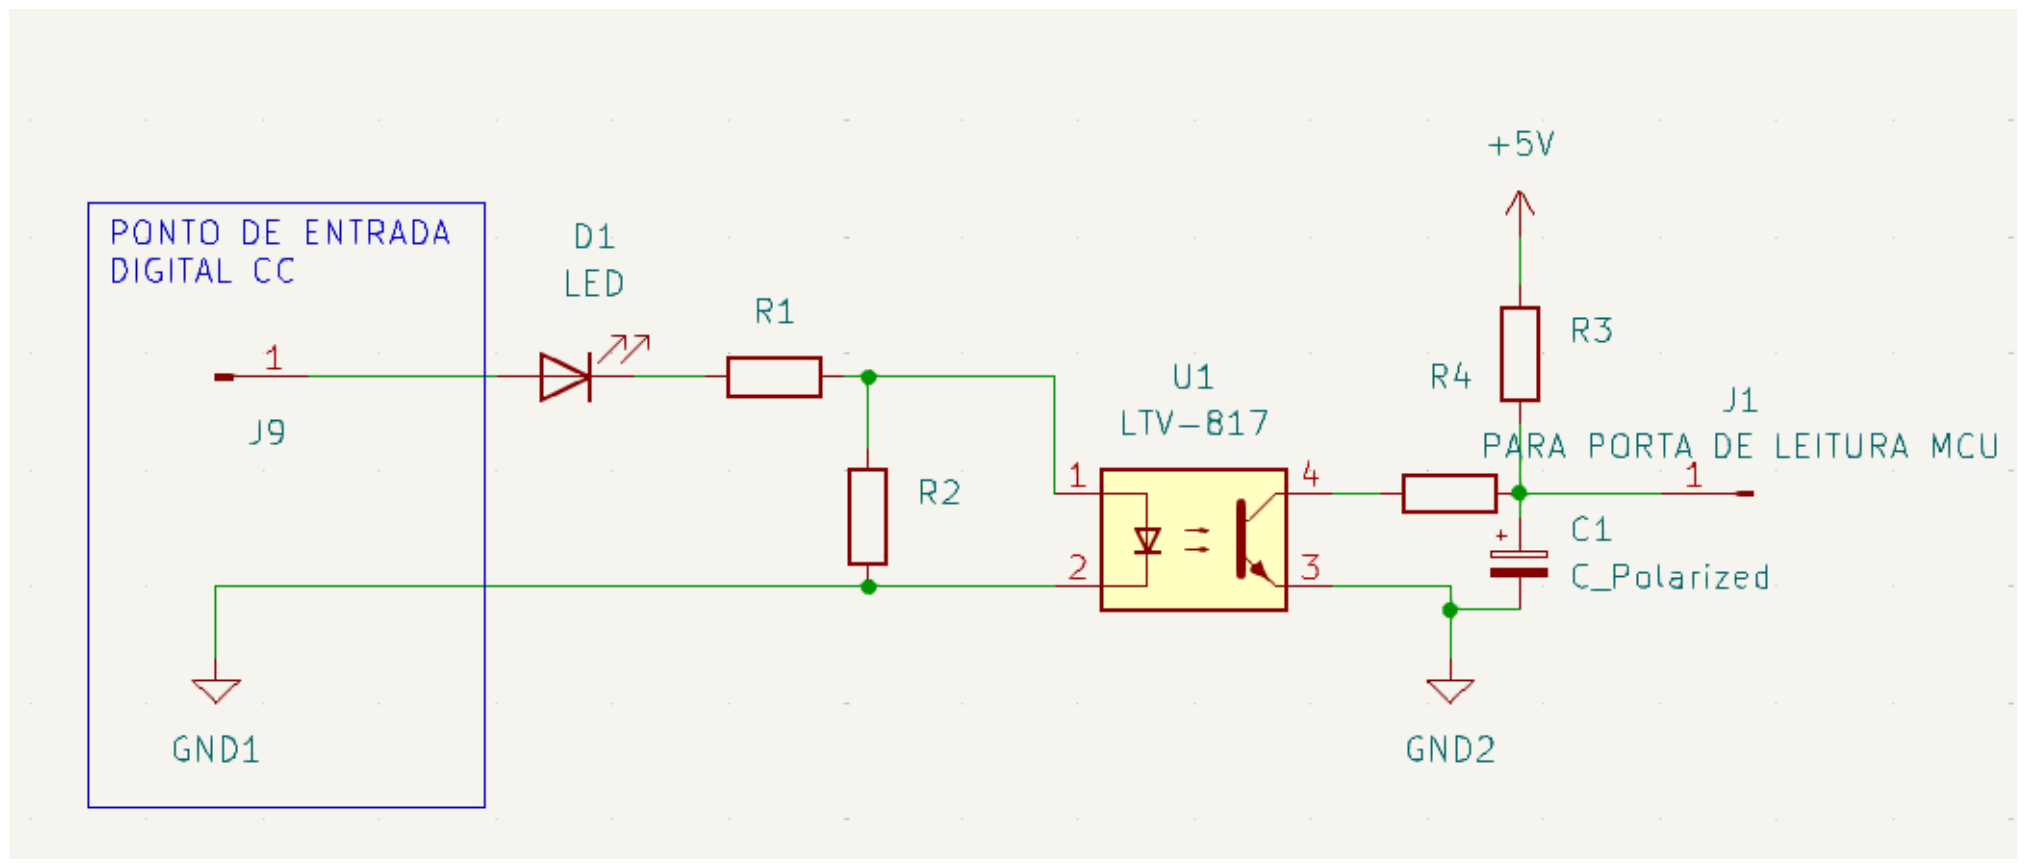
\includegraphics[max width=\linewidth,max height=0.82\textheight]{figuras/figura-79.png}
\label{fig:79}
\caption{Figura 79: Exemplo esquemático para sinal discreto de campo tipo P}
\end{figure}

Um aspecto importante a ser considerado no esquema das entradas é que a parte lógica do circuito é desacoplada do sinal de entrada através de um acoplador óptico, o que assegura a integridade do circuito, caso ocorram problemas com o sinal de entrada, além de aumentar a imunidade a ruídos do sistema.

No fotoacoplador existe um filtro formado por C1, R3 e R4, este filtro fará com que ruídos existentes na alimentação, típicas de ambientes de redes elétricas industriais, não causem um acionamento indevido na porta do MCU, devido ao filtro, normalmente as entradas digitais não deverão responder a uma freqüência maior que 1 kHz, exceto naquelas entradas especiais de contadores rápidos.

\hypertarget{entradas-digitais-em-c.a.}{%
\section{Entradas digitais em C.A.}\label{entradas-digitais-em-c.a.}}

Semelhante às entradas de corrente contínua, as entradas digitais de corrente alternada leem sinais do processo, oferecendo a vantagem de permitir maior distância entre o MCU e o transdutor devido à melhor relação sinal/ruído em tensões de 110 V ou 220 V. Geralmente, em distâncias superiores a 50 m em ambientes ruidosos, é recomendável considerar o uso de entradas CA. Contudo, ao trabalhar com níveis de tensão alternada, é fundamental adotar cuidados extras com a isolação geral da instalação para garantir segurança e confiabilidade.

\begin{figure}[H]
\centering
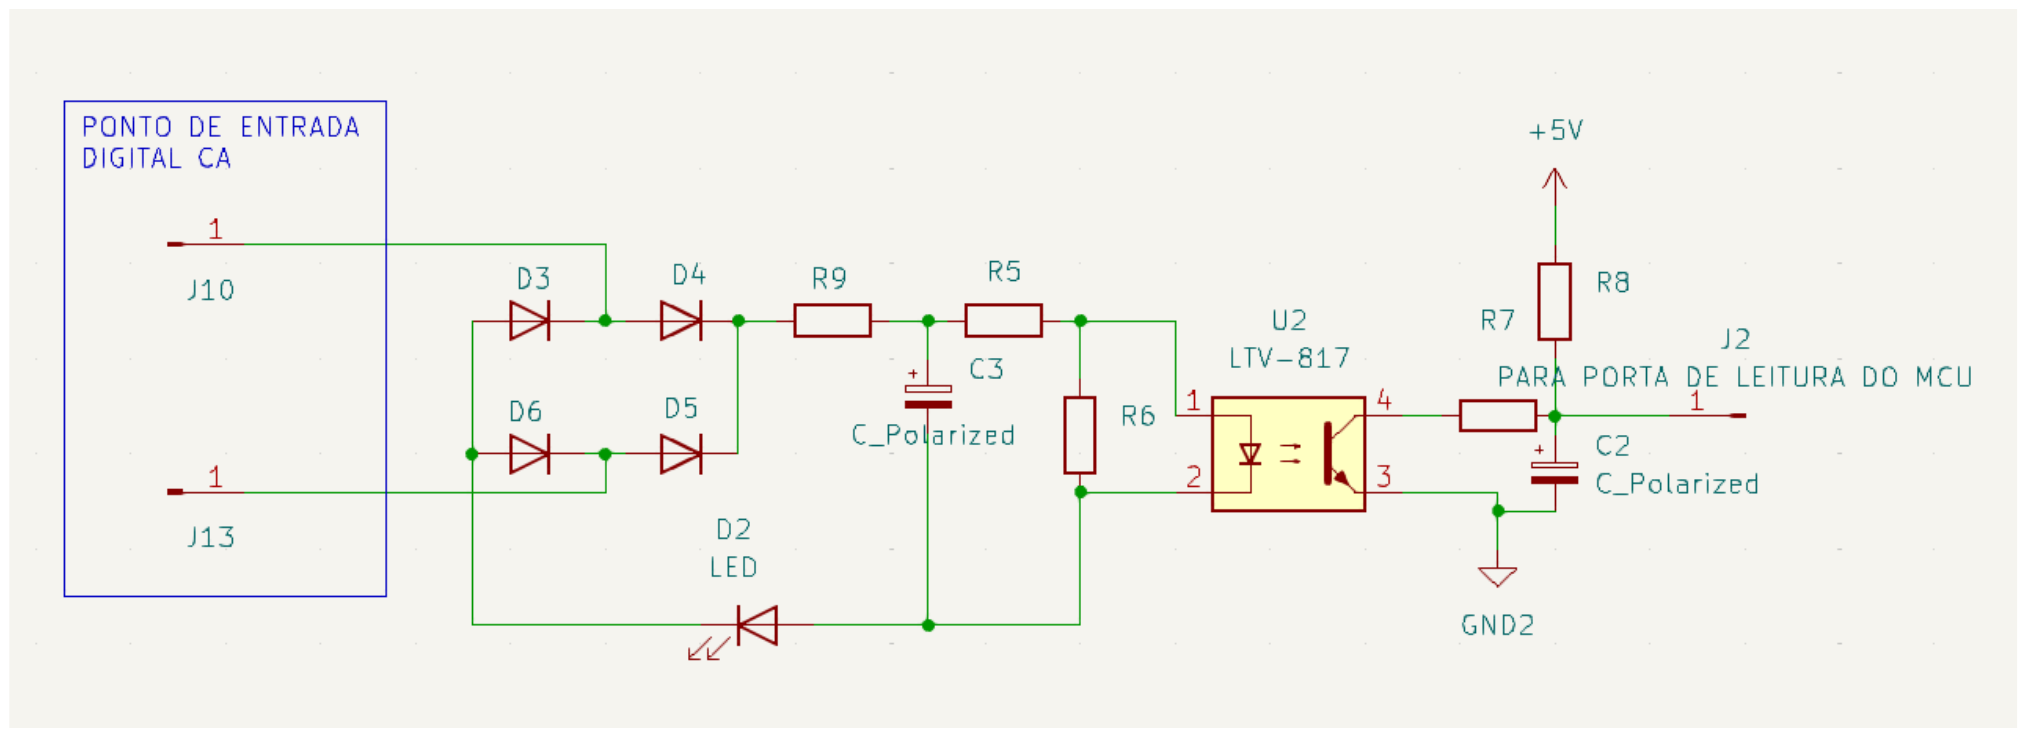
\includegraphics[max width=\linewidth,max height=0.82\textheight]{figuras/figura-80.png}
\label{fig:80}
\caption{Figura 80: Exemplo esquemático para sinal CA discreto de campo}
\end{figure}

\hypertarget{sauxedda-digitais-em-c.c.}{%
\section{Saída digitais em C.C.}\label{sauxedda-digitais-em-c.c.}}

No exemplo do esquemático deve-se ligar a carga entre o potencial negativo da fonte de alimentação de 24 VCC e o ponto de saída (J4 e J5). A figura a seguir exemplifica o circuito de uma saída digital tipo P.

\begin{figure}[H]
\centering
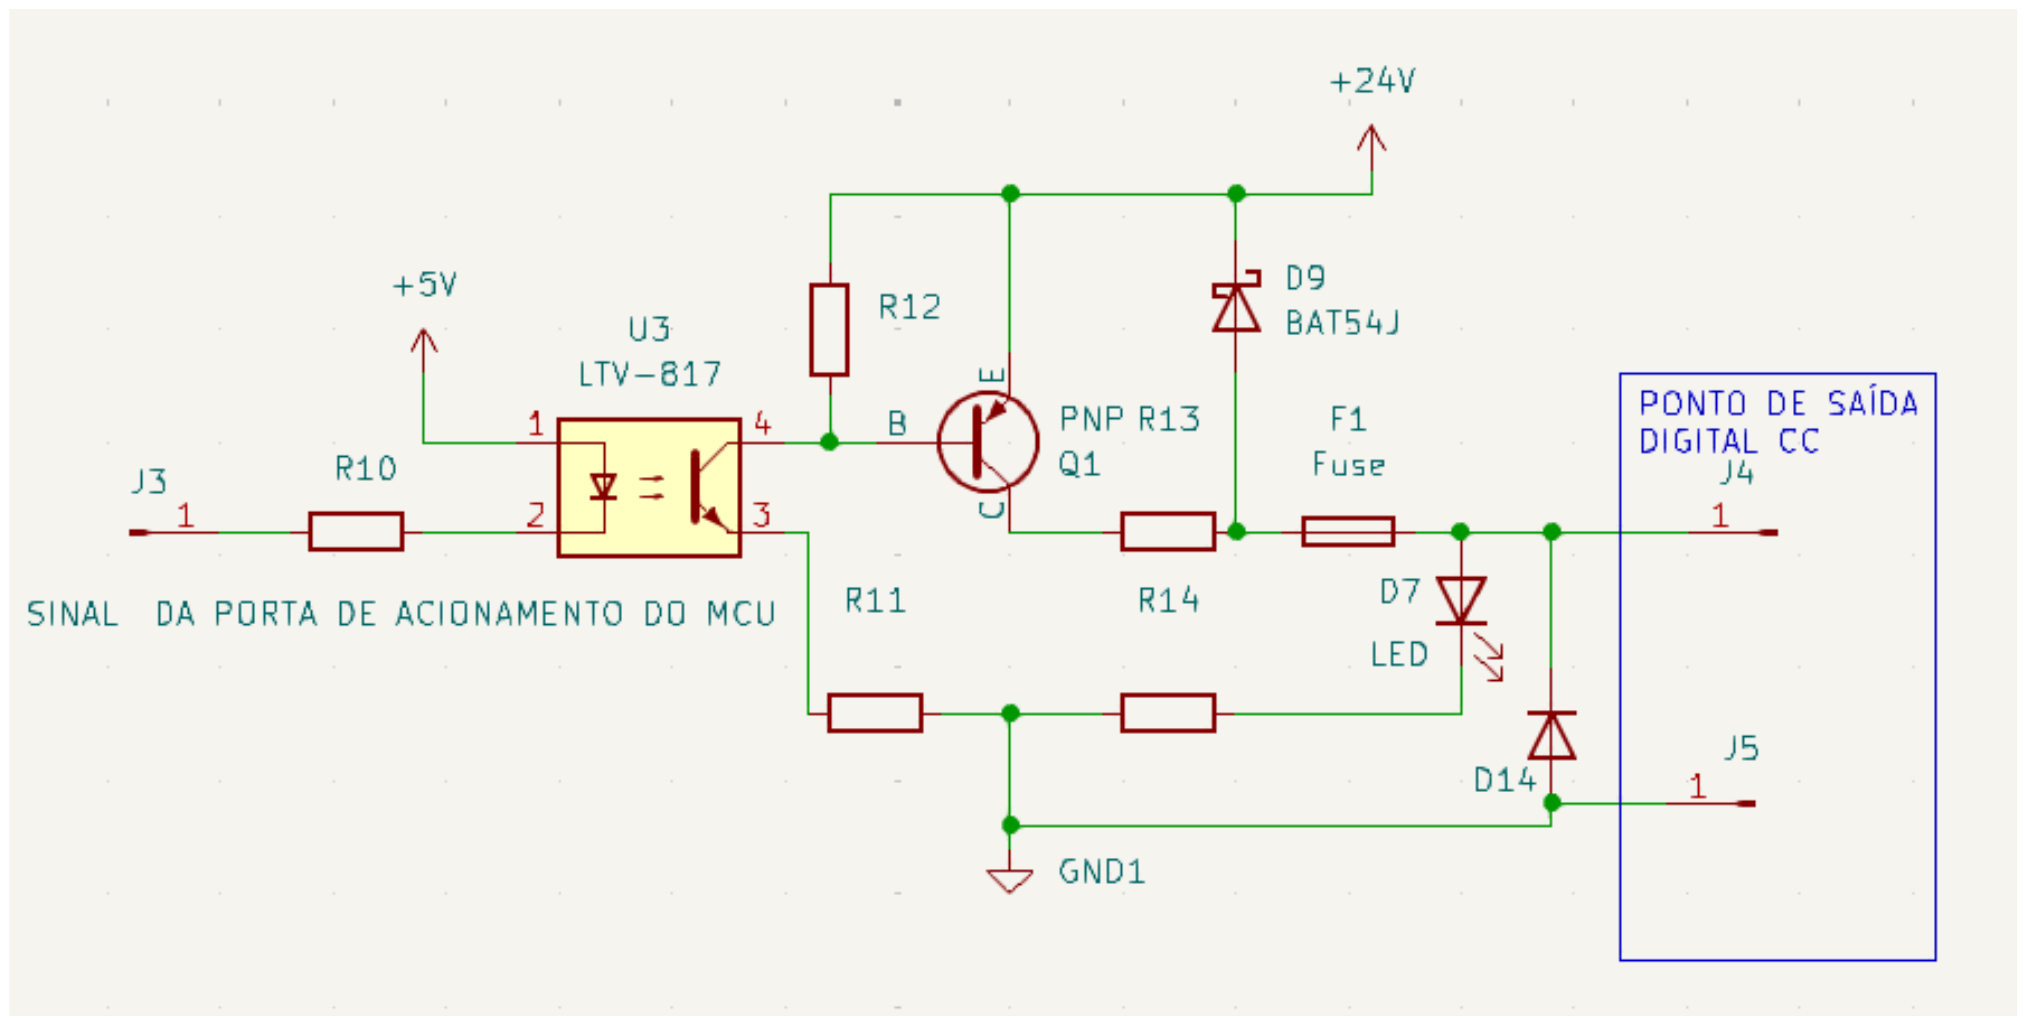
\includegraphics[max width=\linewidth,max height=0.82\textheight]{figuras/figura-81.png}
\label{fig:81}
\caption{Figura 81: Exemplo esquemático para saída digital CC}
\end{figure}

\hypertarget{sauxedda-digitais-em-c.a.-com-triac}{%
\section{Saída digitais em C.A. com TRIAC}\label{sauxedda-digitais-em-c.a.-com-triac}}

A saída em corrente alternada pode ser usado para acionar diretamente bobinas de contatores CA ou outra carga conforme os dimensionamento dos circuitos de saída. A alimentação normalmente é do tipo full range, ou seja, é possível ligar cargas cuja alimentação esteja entre 90 VAC a 240 VAC. A figura a seguir exemplifica o circuito de uma saída digital em corrente alternada.

\begin{figure}[H]
\centering
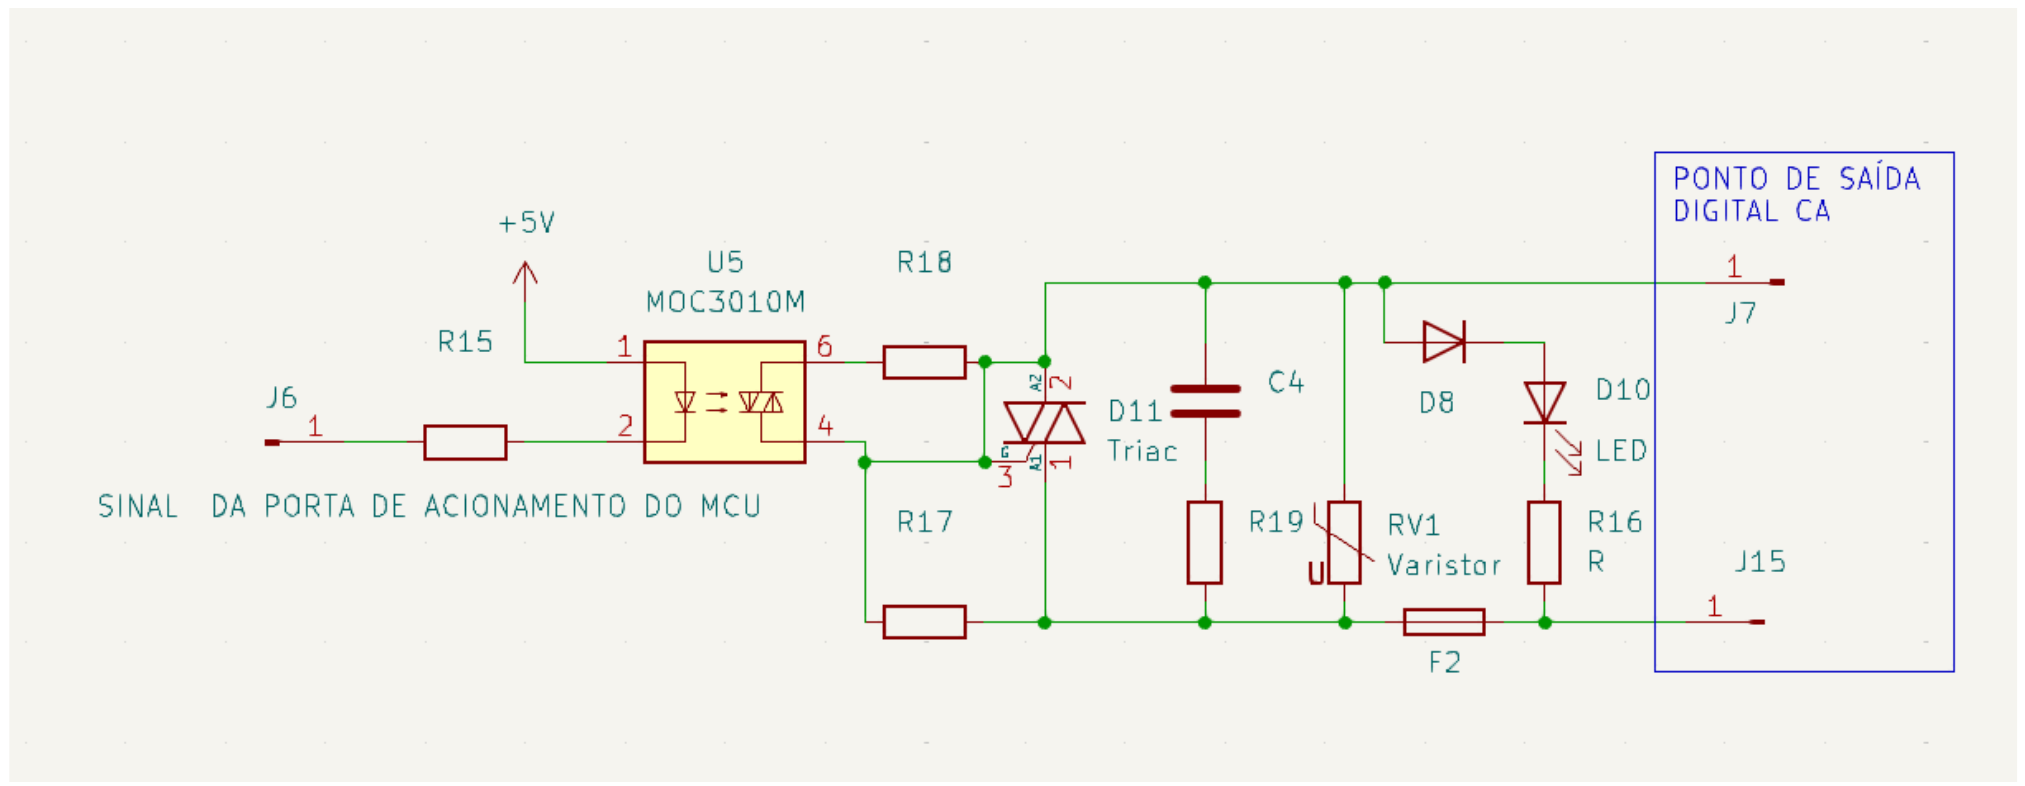
\includegraphics[max width=\linewidth,max height=0.82\textheight]{figuras/figura-82.png}
\label{fig:82}
\caption{Figura 82: Exemplo esquemático para saída digital com acionamento de carga CA. 97}
\end{figure}

No exemplo do circuito pode-se observar alguns elementos importantes:

\begin{itemize}
\tightlist
\item
  Varistor: protege contra o surto de tensão;
\item
  RC: protege contra disparo indevido do TRIAC que está isolado do sistema por acoplador ótico;
\item
  TRIAC Isolado: normalmente é utilizado TRIAC Isolado com função de zero crossing; assim, só ocorrerá o acionamento ou desacionamento no momento da passagem do ``0'' da senóide, evitando, por exemplo, a formação de faíscas quando chaveamos cargas indutivas.
\end{itemize}

\hypertarget{sauxedda-digitais-a-rele}{%
\section{Saída digitais a Rele}\label{sauxedda-digitais-a-rele}}

Esse tipo de saída é bem versátil, pois pode comutar tanto cargas em corrente contínua (C.C.) quanto em corrente alternada (C.A.). No entanto, as saídas a relé apresentam desgaste mecânico proporcional ao número de chaveamentos e à corrente que passa pelos contatos. Para aumentar a vida útil do relé, pode-se utilizar um relé auxiliar externo, inserindo-o entre a saída do esquemático e a carga, ou ainda, intercalar um relé de maior potência ou uma chave estática, o que ajuda a ``proteger'' os contatos do relé interno. As saídas a relé geralmente têm um tempo de resposta mais lento quando comparadas às saídas a transistor ou a TRIAC. A figura a seguir ilustra o circuito de uma saída com contato seco ou relé.

\begin{figure}[H]
\centering
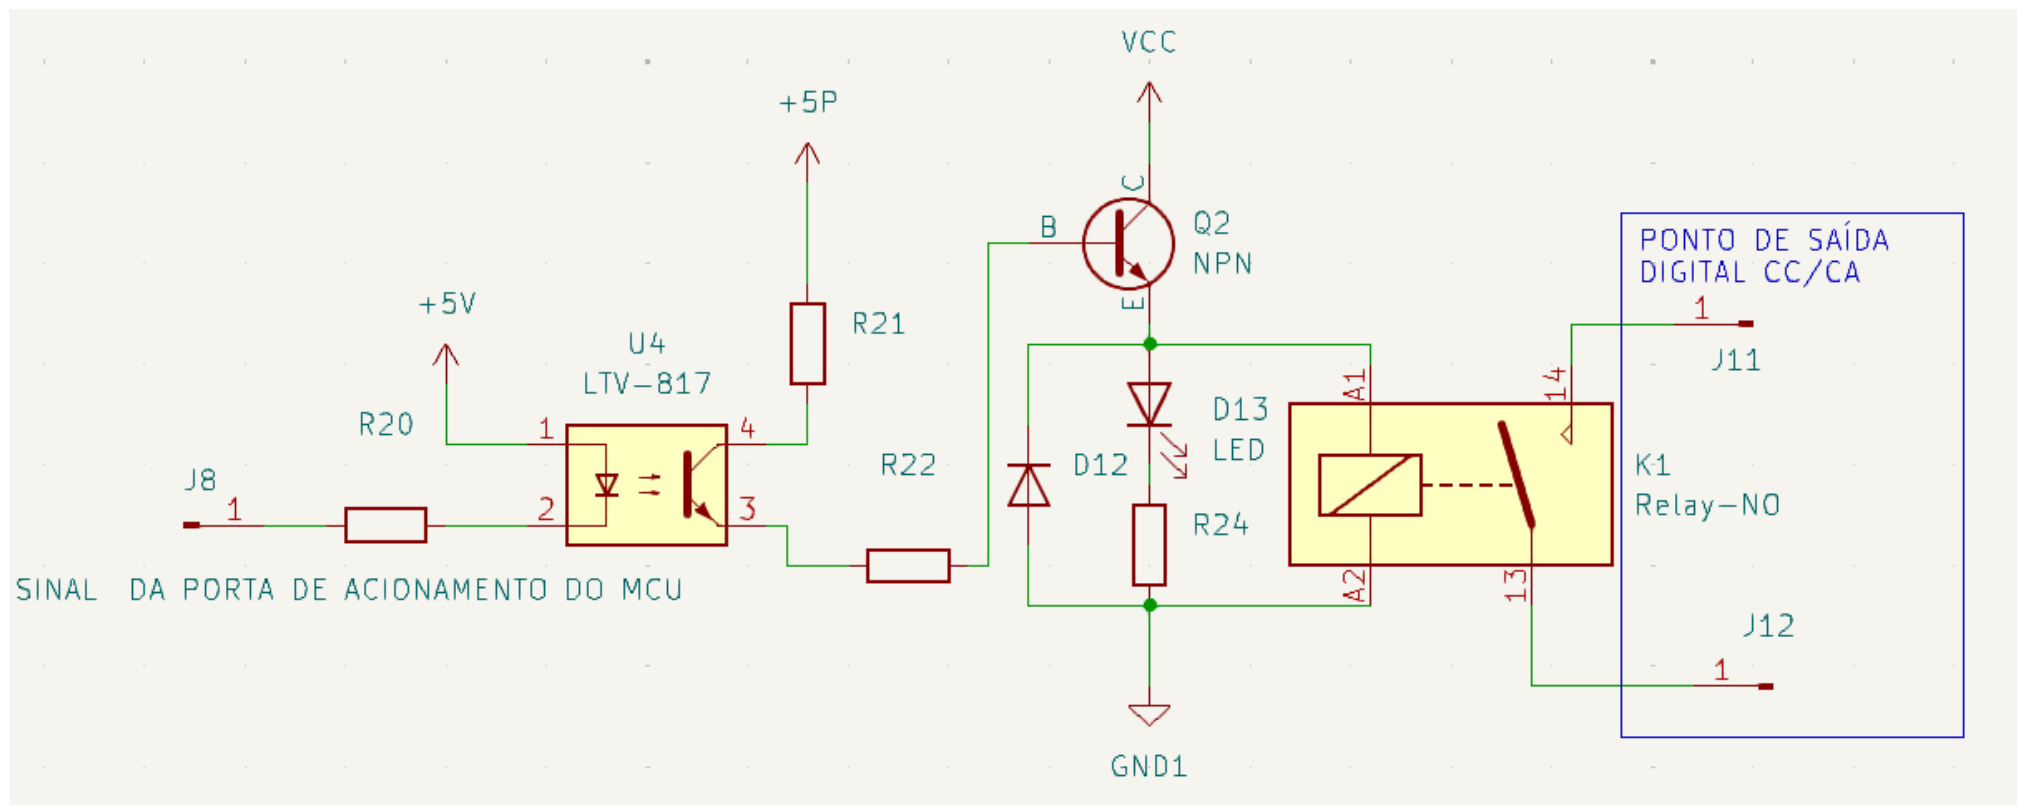
\includegraphics[max width=\linewidth,max height=0.82\textheight]{figuras/figura-83.png}
\label{fig:83}
\caption{Figura 83: Exemplo esquemático para saída digital com acionamento de carga CA ou CC}
\end{figure}

\hypertarget{referuxeancias-web}{%
\chapter*{Referências WEB}
\addcontentsline{toc}{chapter}{Referências WEB}}

\begin{itemize}
\tightlist
\item
  \url{https://jlcpcb.com}
\item
  \url{https://docs.kicad.org/8.0/en/kicad/kicad.html}
\item
  \url{https://www.protoexpress.com/tools/}
\item
  \url{https://blog.raisa.com.br/analise-do-processo-de-fabricacao-de-placas-de-} circuito-impresso-pcb/
\item
  \url{https://embarcados.com.br/acabamento-de-superficie-em-pci/}
\item
  \url{https://embarcados.com.br/10-mandamentos-da-pcb/\#1-Planos-de-Terra-de-} uma-PCB
\item
  \url{https://delorenzoglobal.com/}
\item
  \url{https://youtu.be/NYrRZNzBmsk}
\end{itemize}


\end{document}
